\section{Signal Modeling}
\label{sec:signal_model}
%=== FROM AN but modified. ===%
%The dominant POWHEG ggF process is reweighted to the NNLOPS one, using bins of generated Higgs 
%$p_{T}$ and number of generated jets. More details in \cite{HIG_19_001}.
% TODO:REWORD

\subsection{Signal Normalization}
\label{sec:SignalNormalization}
% TODO:REWORD
The normalization of the Higgs boson signal is obtained from simulation, 
looking at the expected signal yields in the range [105, 140] GeV, 
for five simulated mass points (120, 124, 125, 126, and 130 GeV).
A second order polynomial function is used to extract the dependence of the normalization from $m_{H}$.
Fits are performed separately for each production mode, for each decay channel and for each year. 
Examples of the fits are shown in Fig.~\ref{fig:signal_normalization}
\begin{multiFigure}
    \centering
    \addFigure{0.48}{../../higgsmassmeasurement/AN-19-248/Figures/SignalModelling/Signal_Normalisation/NoZ1/2016pre_ggH_yield_workinprogress.pdf}
    \addFigure{0.48}{../../higgsmassmeasurement/AN-19-248/Figures/SignalModelling/Signal_Normalisation/NoZ1/2016post_ggH_yield_workinprogress.pdf}
    \addFigure{0.48}{../../higgsmassmeasurement/AN-19-248/Figures/SignalModelling/Signal_Normalisation/NoZ1/2017_ggH_yield_workinprogress.pdf}
    \addFigure{0.48}{../../higgsmassmeasurement/AN-19-248/Figures/SignalModelling/Signal_Normalisation/NoZ1/2018_ggH_yield_workinprogress.pdf}
    \captionof{figure}
        [Normalization fit for the ggH signal in different final states]
        {Normalization fit for the ggH signal in different final states (expected yield \vs $\mH / 125\GeV$) for all years during Run 2.
        \;A) 2016 pre-VFP.
        \;B) 2016 post-VFP.
        \;C) 2017.
        \;D) 2018.
        }
    \label{fig:signal_normalization}
\end{multiFigure}
%%%%%%% 
%%%%%%% 
% plots about normalisation will be shown only for 1D_VXBS_Z1 configuration
%%%%%%% 
%%%%%%% 
%
%\begin{figure}[!htbp]
%	\begin{center}
%   		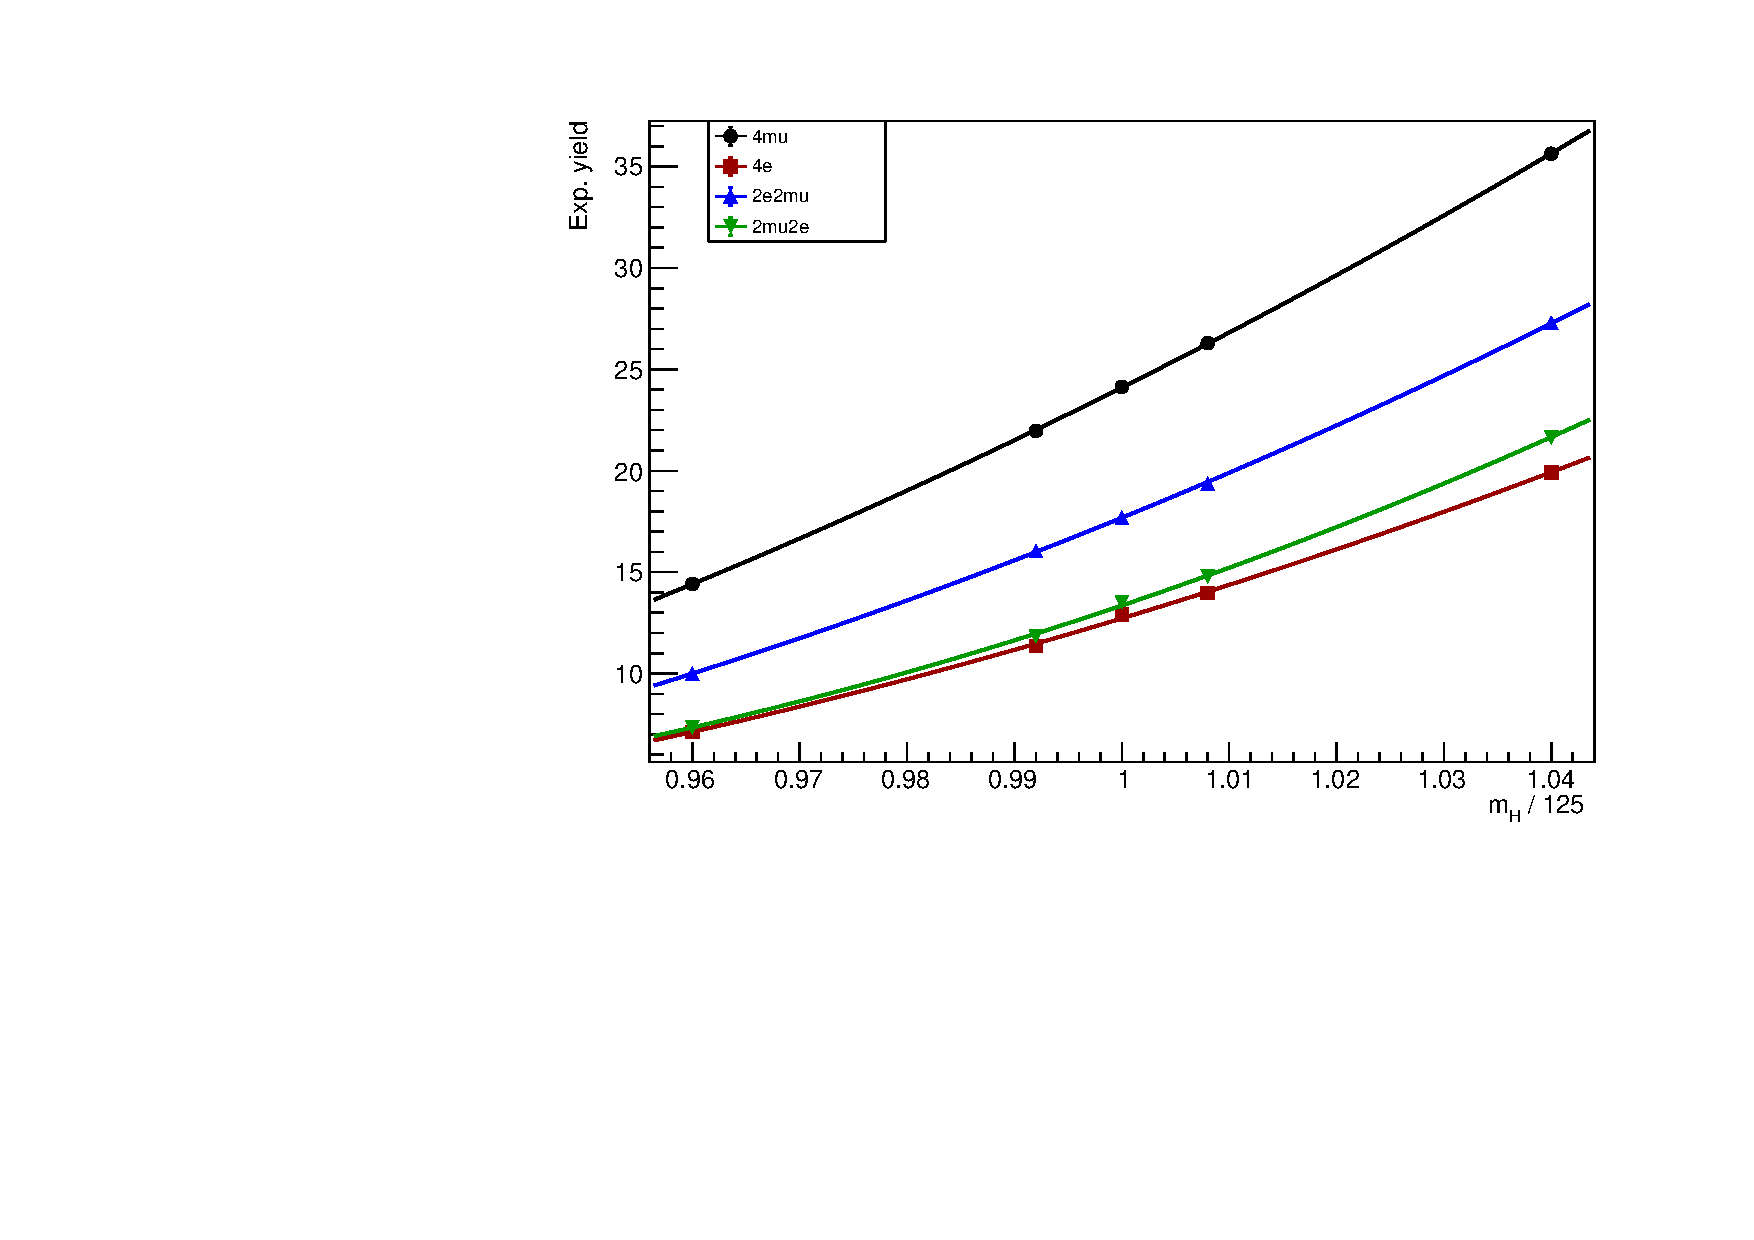
\includegraphics[width=0.3\textwidth]{Figures/SignalModelling/Signal_Normalisation/NoZ1/2017_ggH_yield.pdf}
%		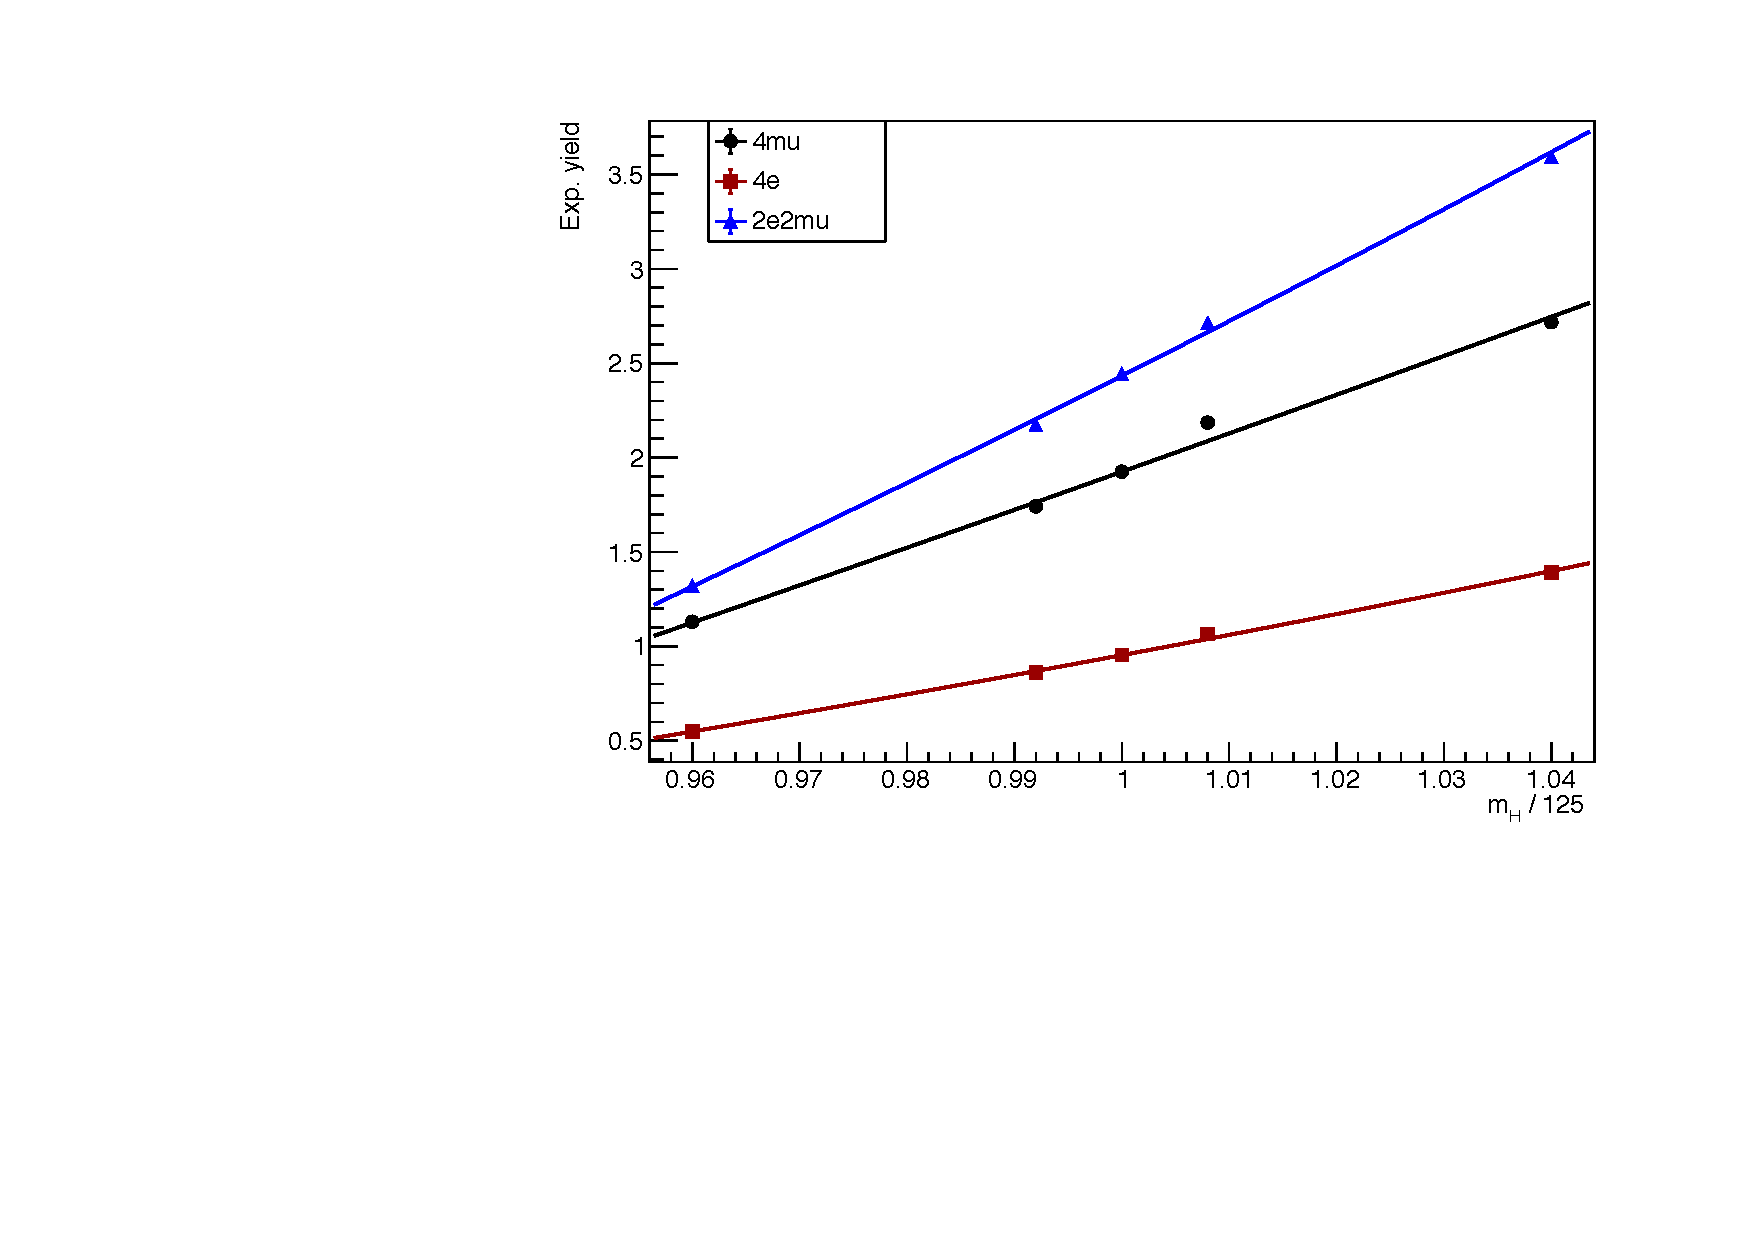
\includegraphics[width=0.3\textwidth]{Figures/SignalModelling/Signal_Normalisation/NoZ1/2017_VBF_yield.pdf} 
%		\includegraphics[width=0.3\textwidth]{Figures/SignalModelling/Signal_Normalisation/NoZ1/2017_ZH_yield.pdf}
%		\caption{Normalization fit in 2017, for different decay channels, as a function
%		of mass, for ggH on the left, VBF in the middle, ZH on the right.}
%	\label{signal_normalization_2017}
%	\end{center}
%\end{figure}
%
%\begin{figure}[!htbp]
%	\begin{center}
%   		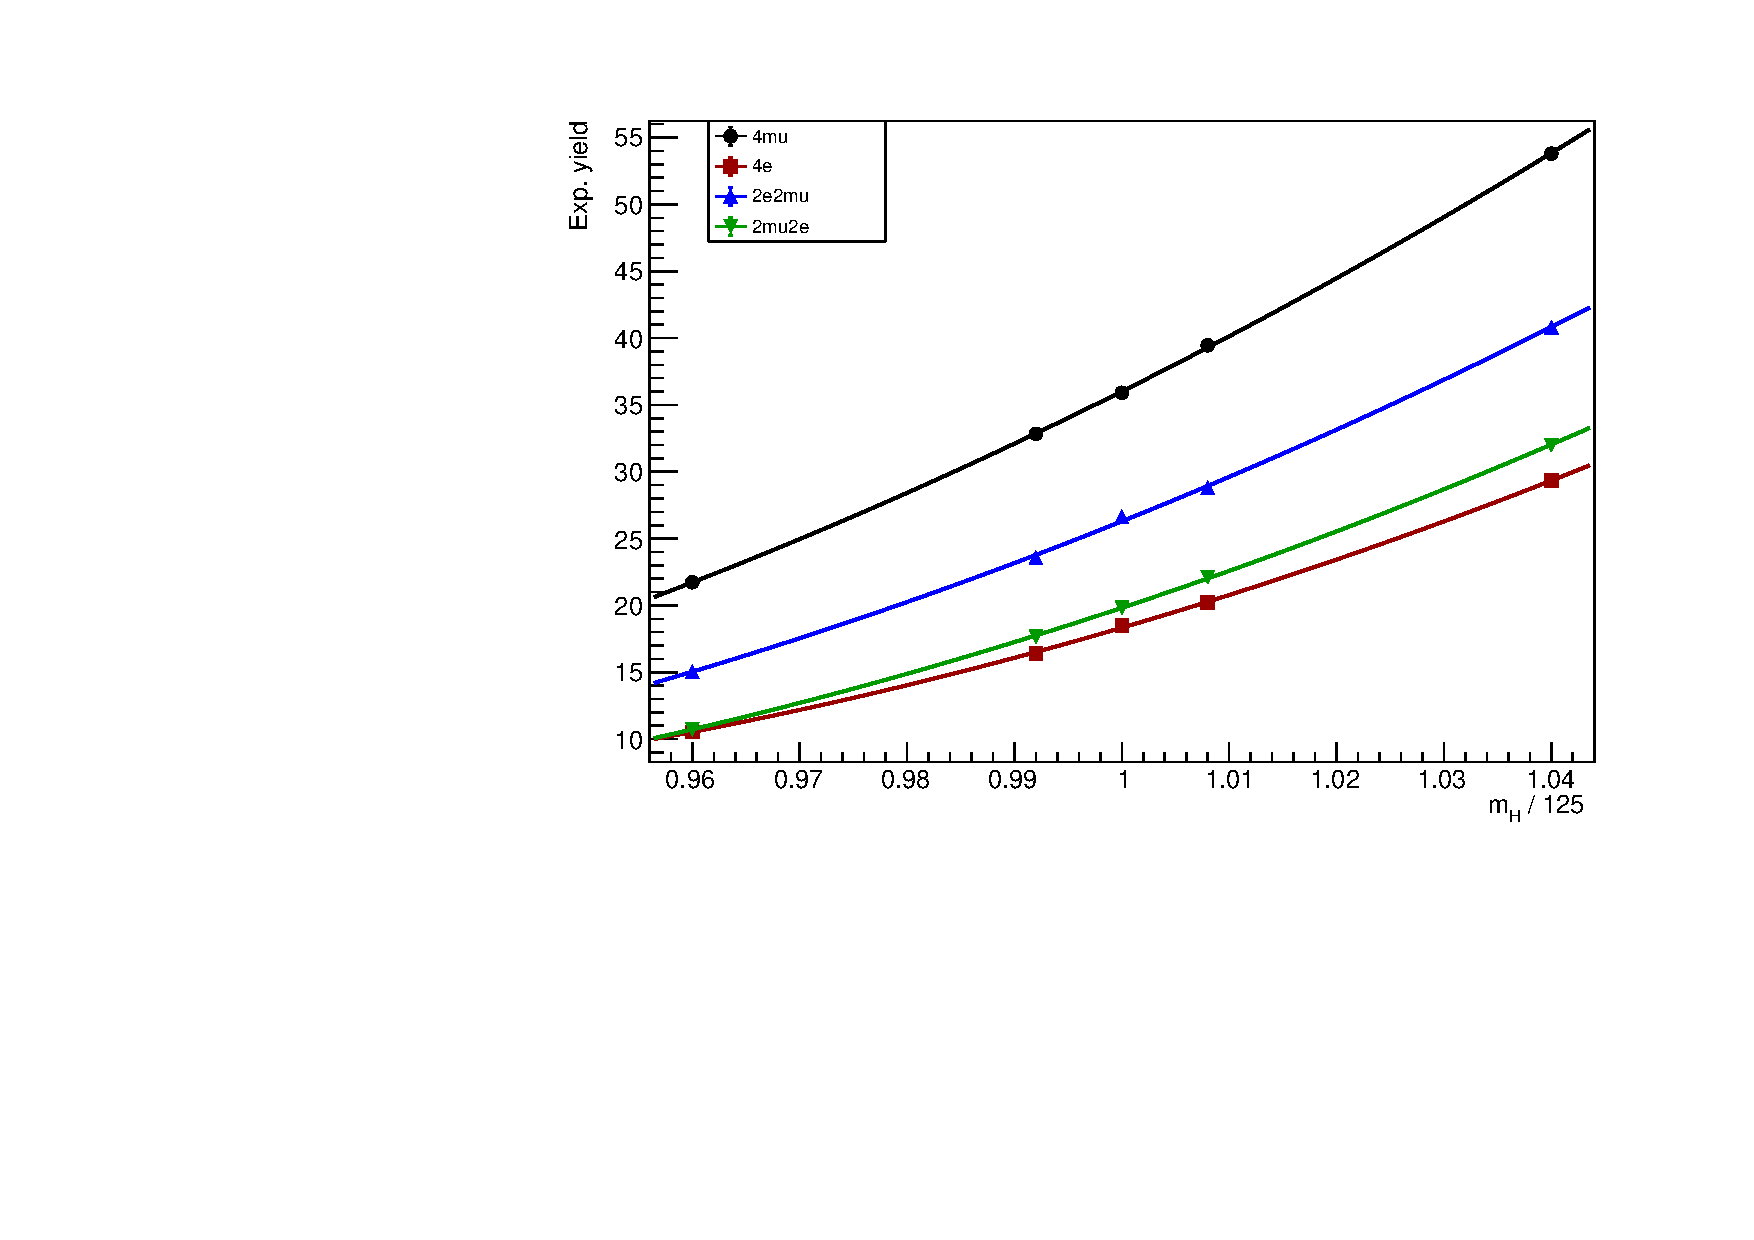
\includegraphics[width=0.3\textwidth]{Figures/SignalModelling/Signal_Normalisation/NoZ1/2018_ggH_yield.pdf}
%		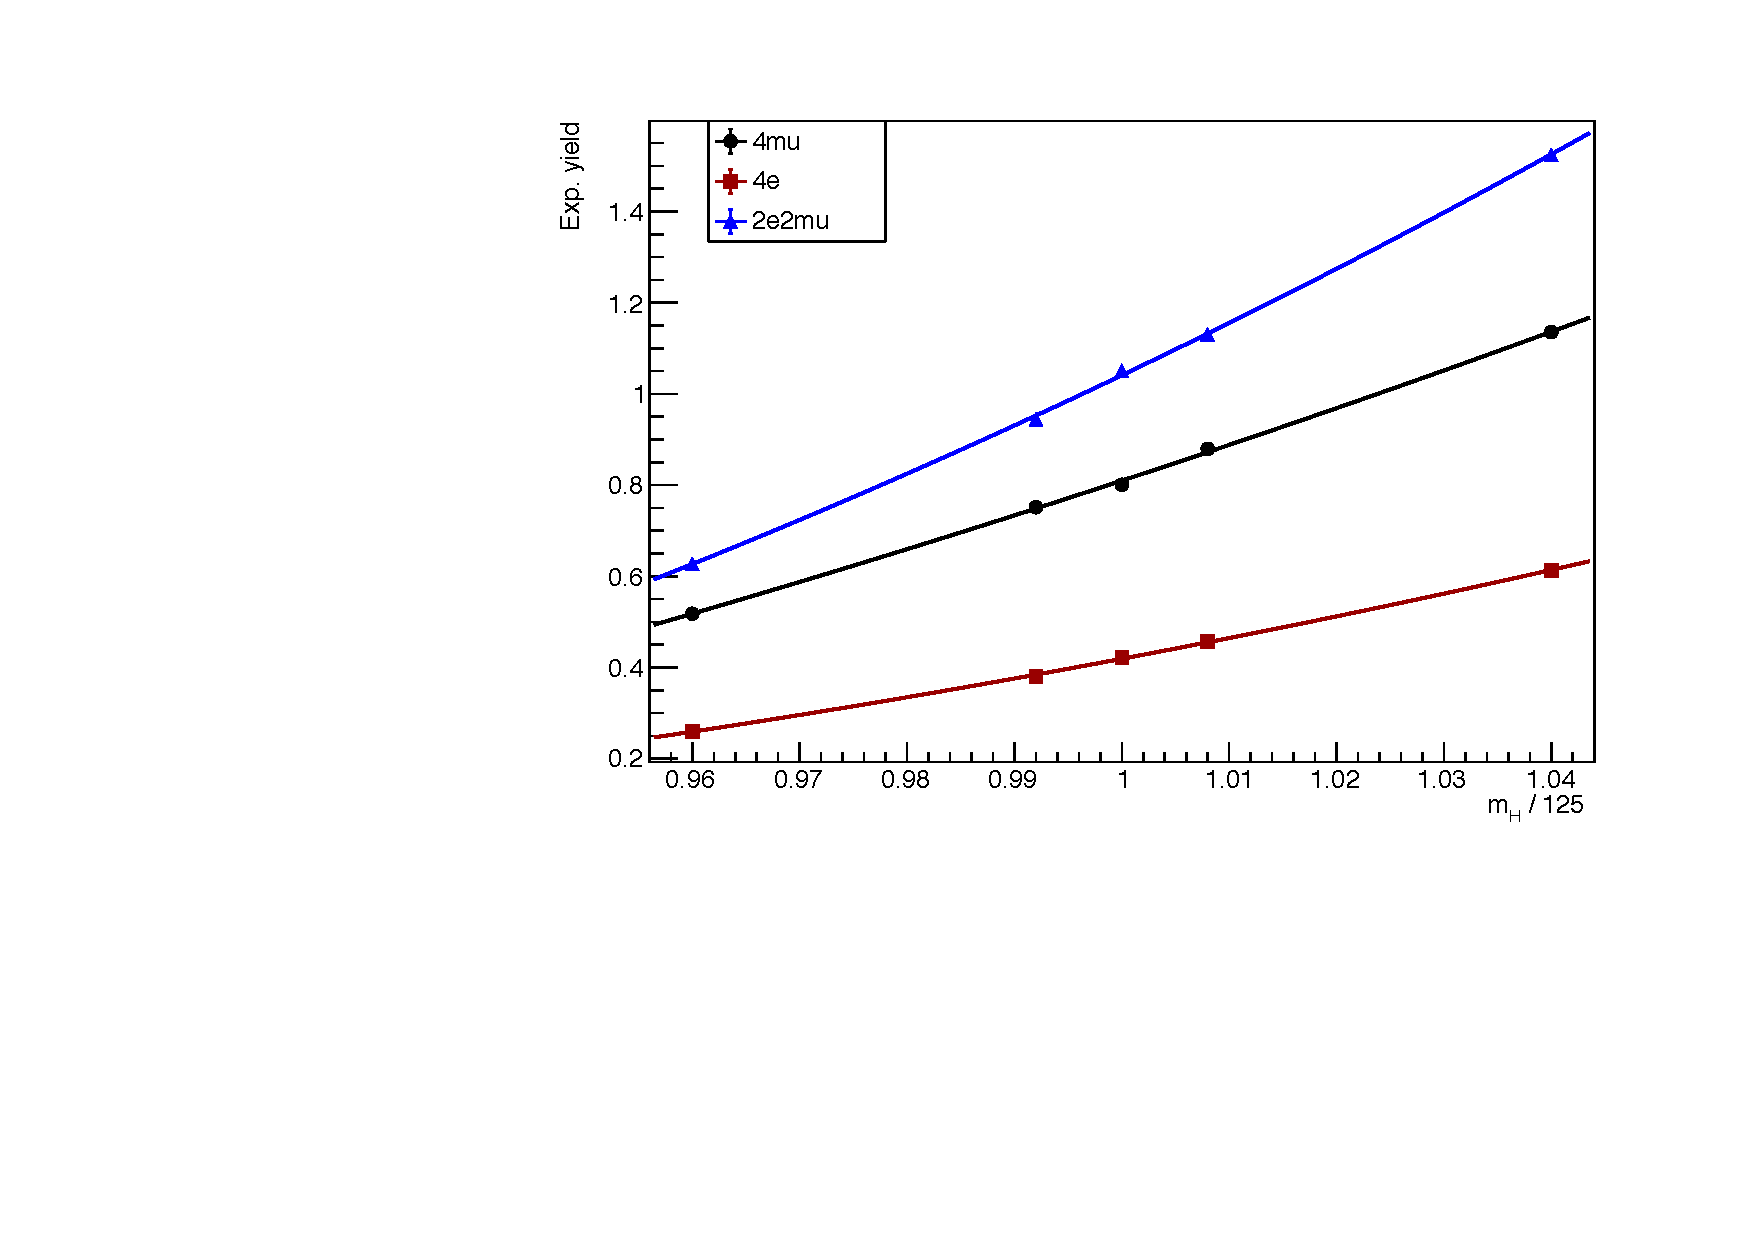
\includegraphics[width=0.3\textwidth]{Figures/SignalModelling/Signal_Normalisation/NoZ1/2018_WH_yield.pdf} 
%		\includegraphics[width=0.3\textwidth]{Figures/SignalModelling/Signal_Normalisation/NoZ1/2018_ttH_yield.pdf}
%		\caption{Normalization fit in 2018, for different decay channels, as a function
%		of mass, for ggH on the left, WH in the middle, ttH on the right.}
%	\label{signal_normalization_2018}
%	\end{center}
%\end{figure}

\subsection{Parameterizing the Signal Line Shape}
\label{sec:SignalParametrization}
% TODO:REWORD
The signal lineshape is obtained from the fit of the Higgs boson mass distribution, 
in the range [105, 140]\GeV, using a double-sided Crystal Ball (DSCB) function, which has 6 parameters.
%This function has six independent parameters, 
%with a Gaussian core ($\sigma_{m}$) that describes the four-lepton mass resolution function and 
%the systematic mass shift ($\Delta m_{H}$) of the peak, and the left- and right-hand tail 
%originating from leptons emitting brem in the tracker material, present for both electrons and muons, 
%and from the non-Gaussian mis-measurements specific to interactions of electrons with the detector material 
%(each side of the distribution is described by two parameters, n and $\alpha$).\\
Fit parameters $\theta^i$ are derived as a function of \mH, using a first-order polynomial:
%\textbf{Compare first vs second order formula: current results with second one}
\[
\theta^{i}_\text{DSCB} = a^i + b^{i}~(\mH - 125)% + c~(m_{H} - 125)^{2}
\]

First, fitting only the 125\GeV sample, the $a^i$ term for each parameter is extracted ($b^i$ is not yet taken into account).
Then, a second fit is performed:
this time, $a^i$ is fixed to the value found before, while $b^i$ is kept free to float when fitting all five different mass points (120, 124, 125, 126, 130\GeV) simultaneously.

The fit is performed separately, for each production mode, for each decay channel, for each year. 
To take into account the non-resonant contribution in the case of $\PV\PH$ and $\ttbarh$ production modes, the 
DSCB is convoluted with a Landau function that describes the possibility for a 
lepton from the Higgs boson decay to be lost or not selected.\\
%%%%%%% 
%%%%%%% 
% plots about normalisation will be shown only for 1D_VXBS_Z1 configuration
%%%%%%% 
%%%%%%% 
%Examples of the fit procedures are shown in \figurename~\ref{signal_lineshape_2016}, \ref{signal_lineshape_2017}, 
%\ref{signal_lineshape_2018} for 125 GeV sample, and in  \figurename~\ref{signal_lineshape_2016_full_1}, 
%\ref{signal_lineshape_2016_full_2}, \ref{signal_lineshape_2017_full_1}, 
%\ref{signal_lineshape_2017_full_2}, \ref{signal_lineshape_2018_full_1} and  
%\ref{signal_lineshape_2018_full_2}, for the simultaneous fits.
%\begin{figure}[!htbp]
%	\begin{center}
%   		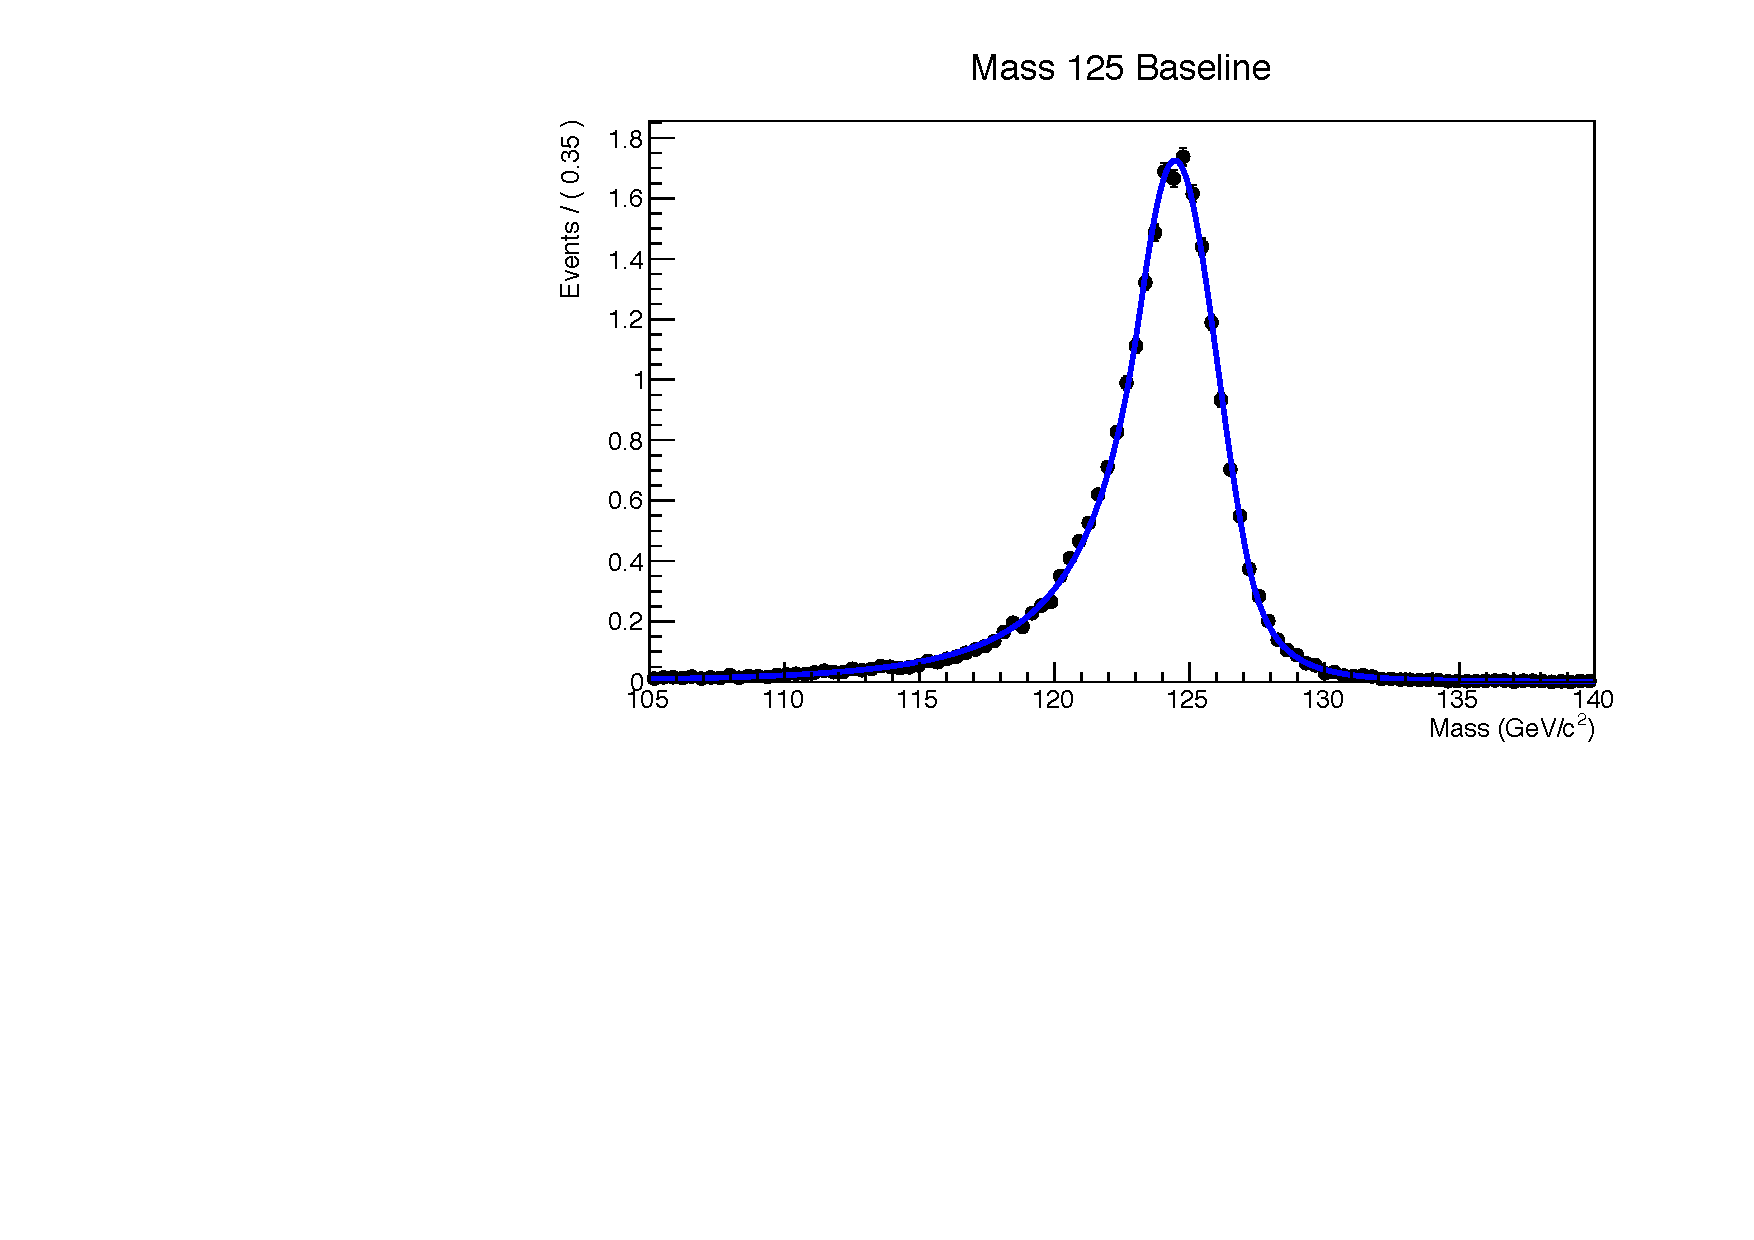
\includegraphics[width=0.3\textwidth]{Figures/SignalModelling/Signal_Parametrization/2016/ggH_2e2mu_2016_125.pdf}
%		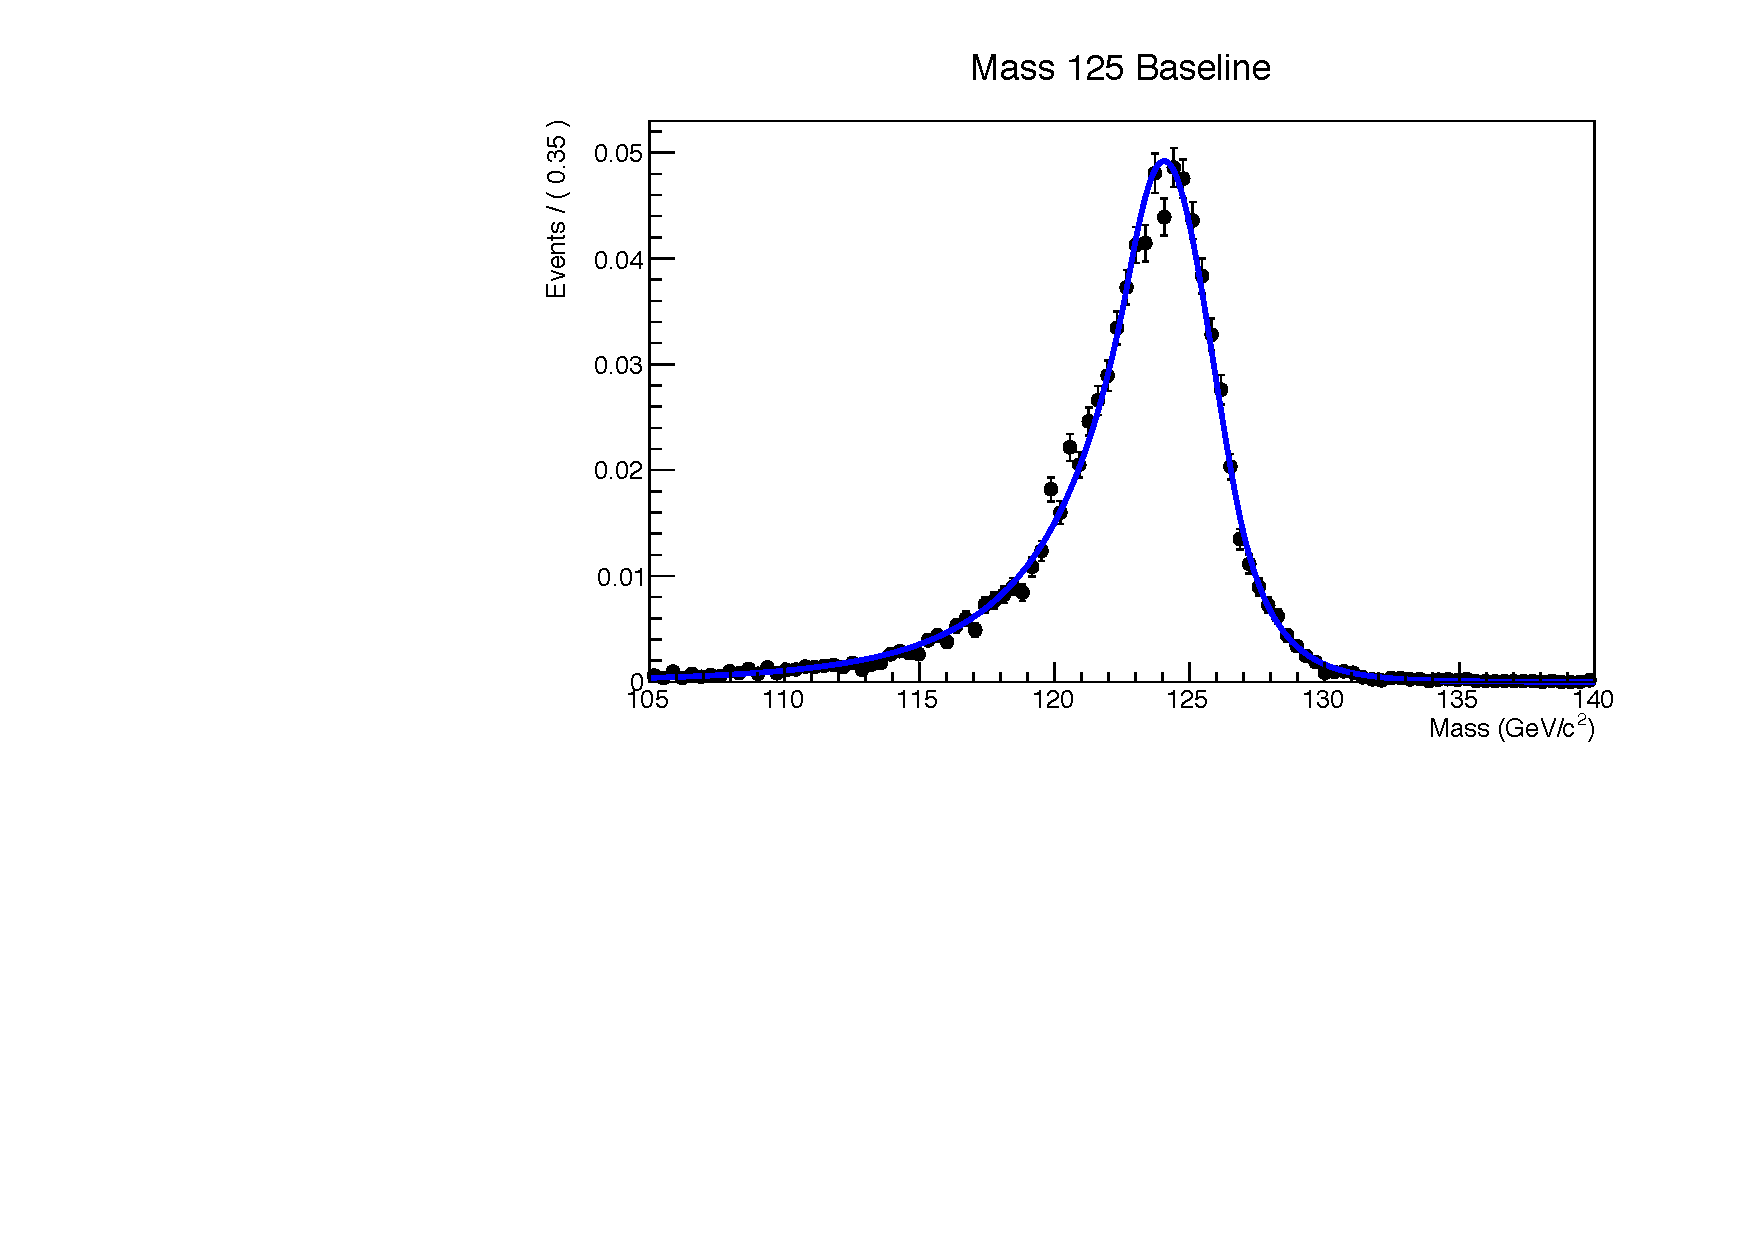
\includegraphics[width=0.3\textwidth]{Figures/SignalModelling/Signal_Parametrization/2016/VBF_4e_2016_125.pdf} 
%%		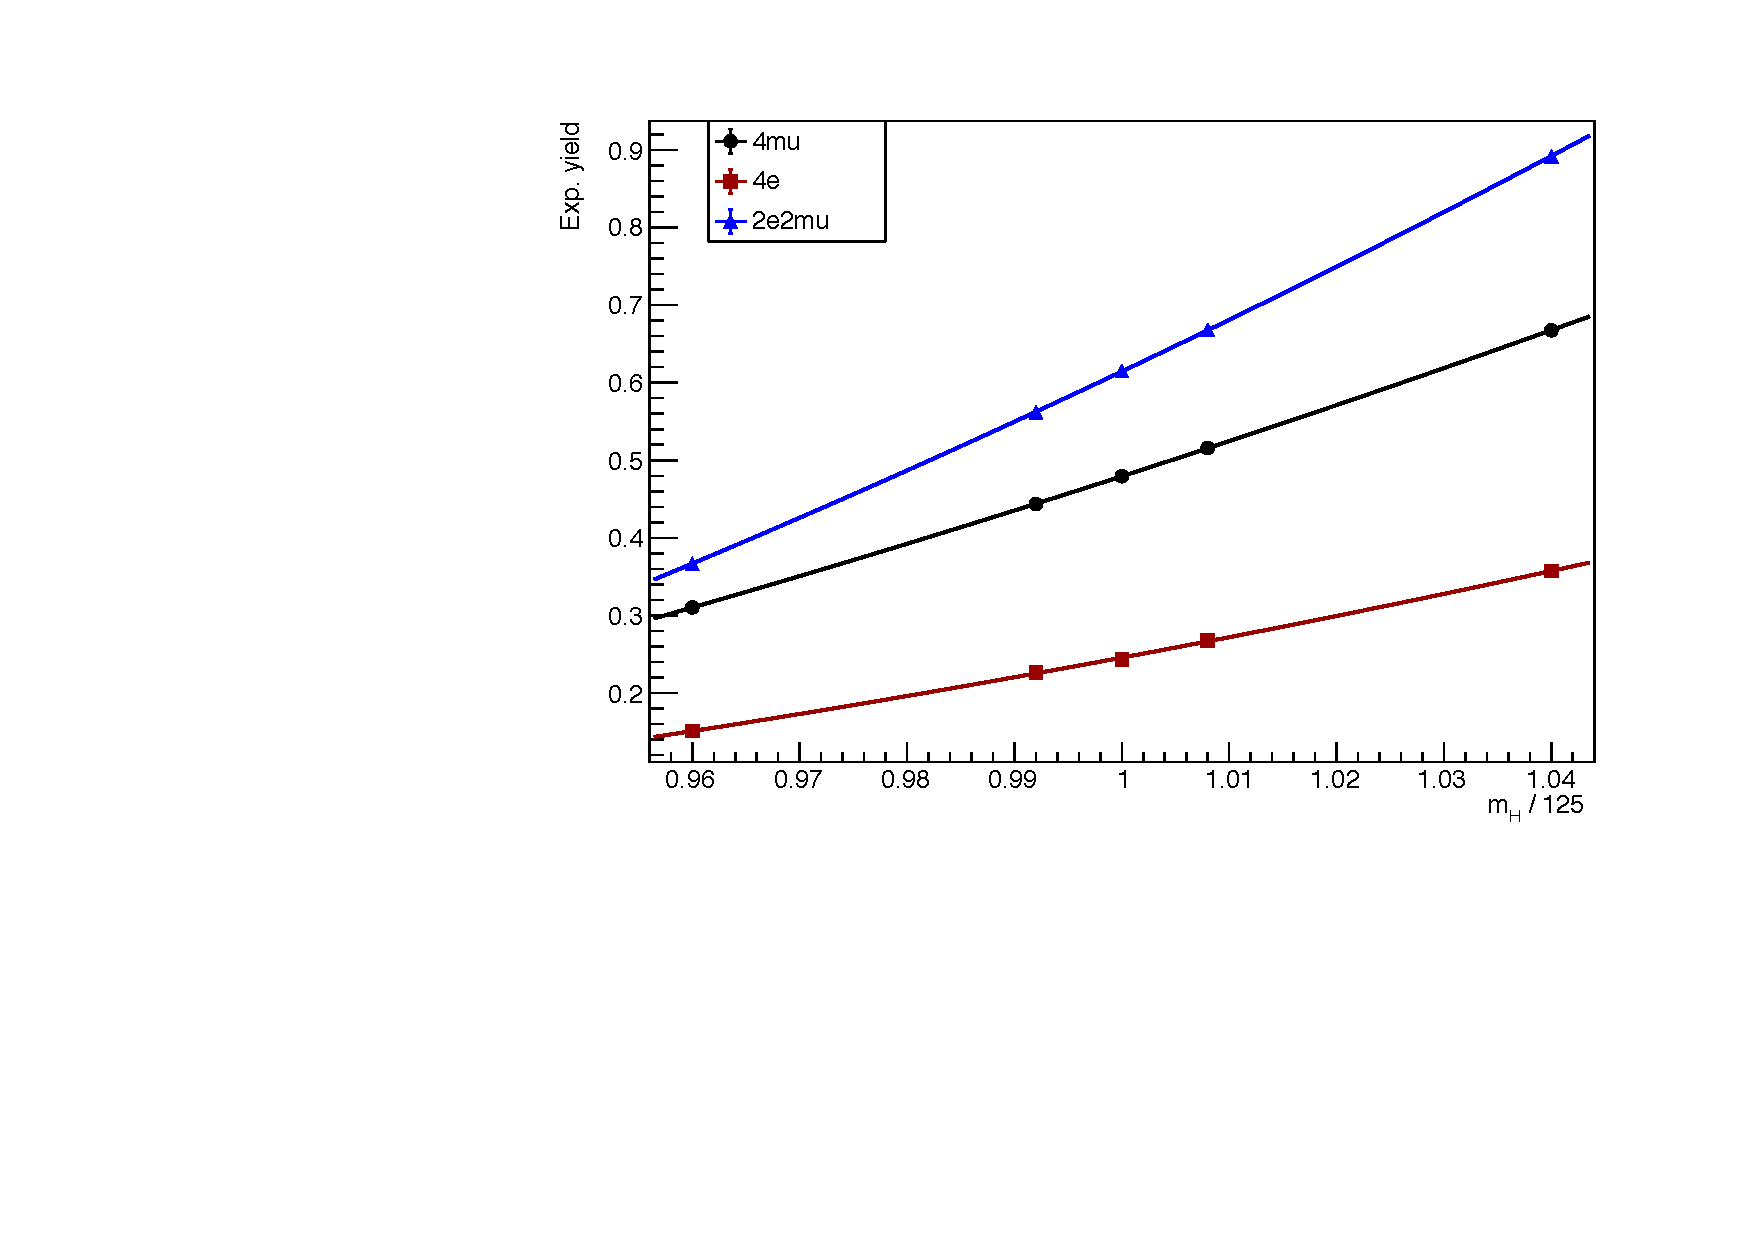
\includegraphics[width=0.3\textwidth]{Figures/SignalModelling/Signal_Parametrization/2016/2016_WH_yield.pdf}
%		\caption{125 GeV fit in 2016: 2e2$\mu$ ggF on the left, 
%		4e VBF on the right.}
%	\label{signal_lineshape_2016}
%	\end{center}
%\end{figure}
%\begin{figure}[!htbp]
%	\begin{center}
%   		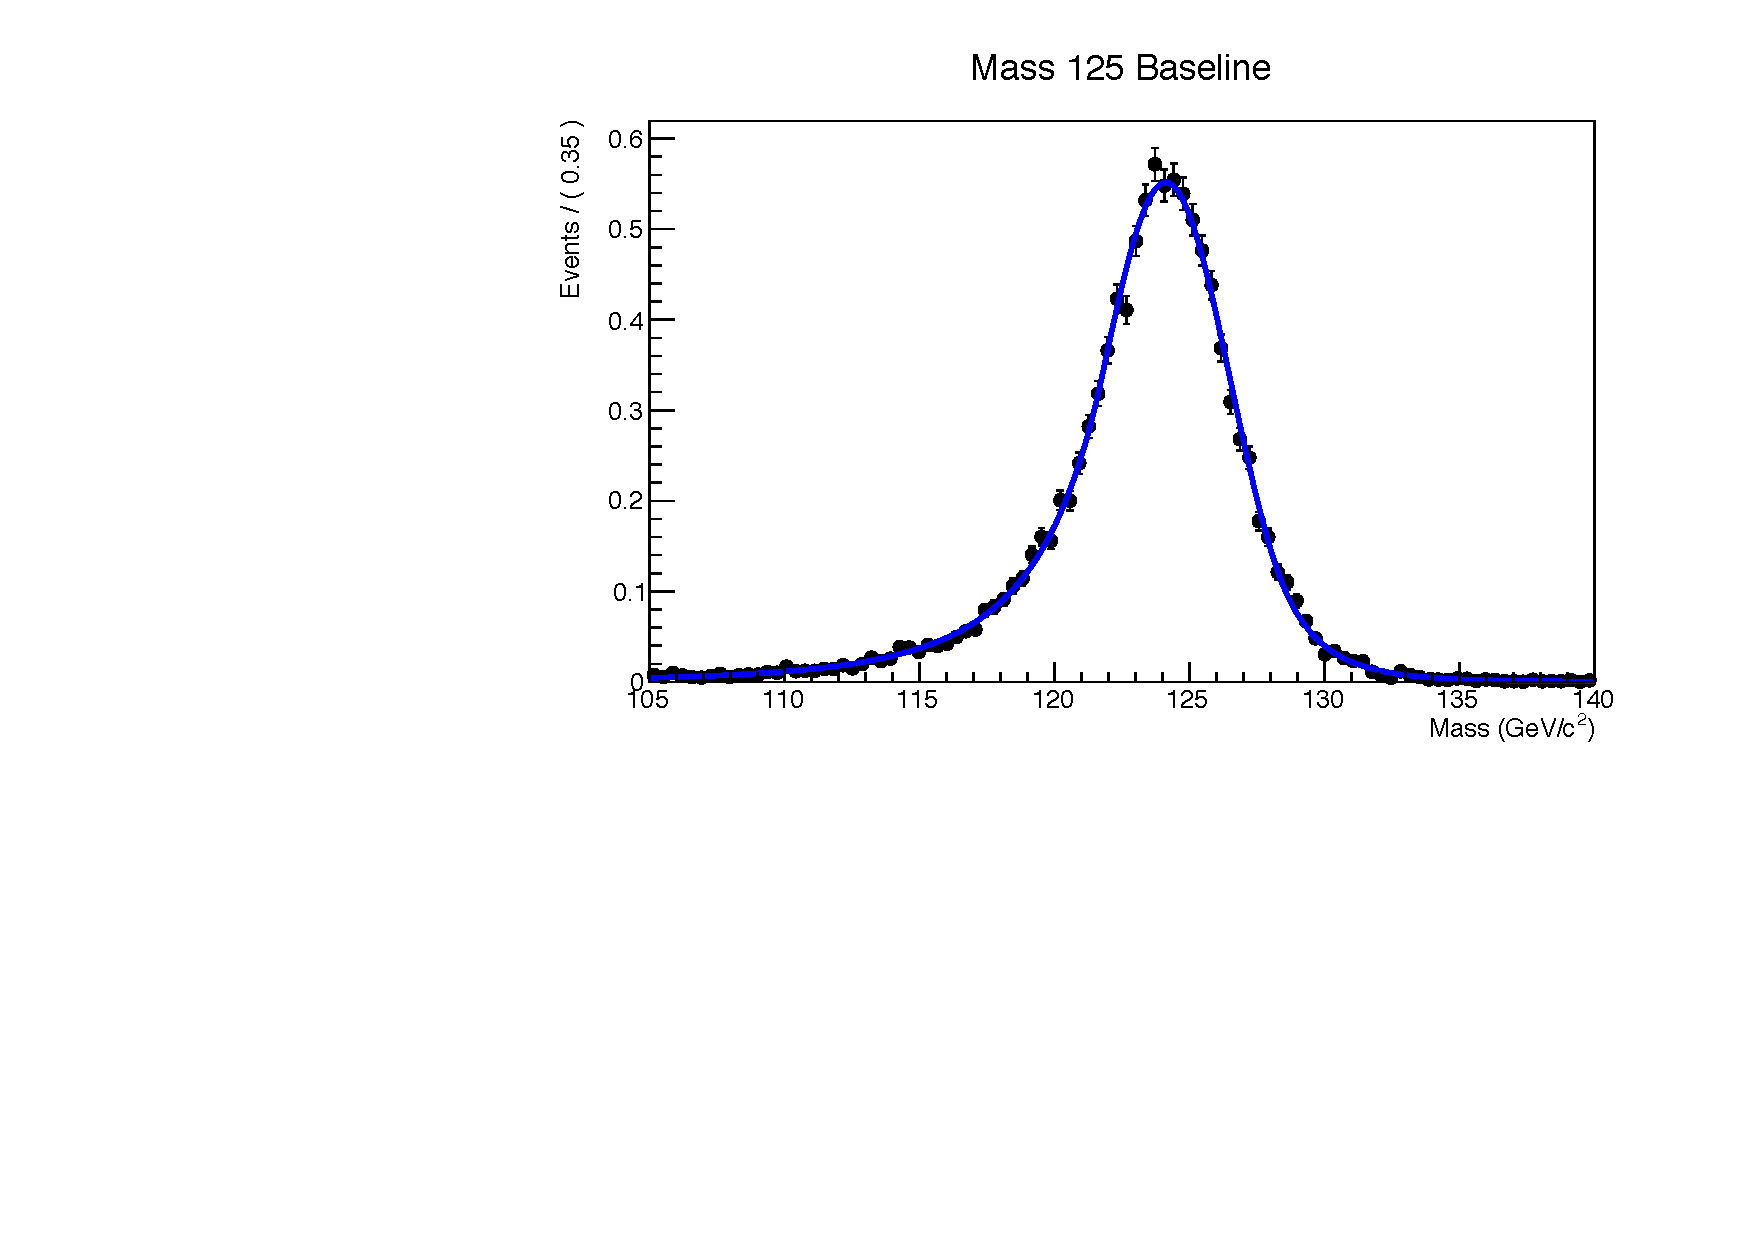
\includegraphics[width=0.3\textwidth]{Figures/SignalModelling/Signal_Parametrization/2017/ggH_4e_2017_125.pdf}
%		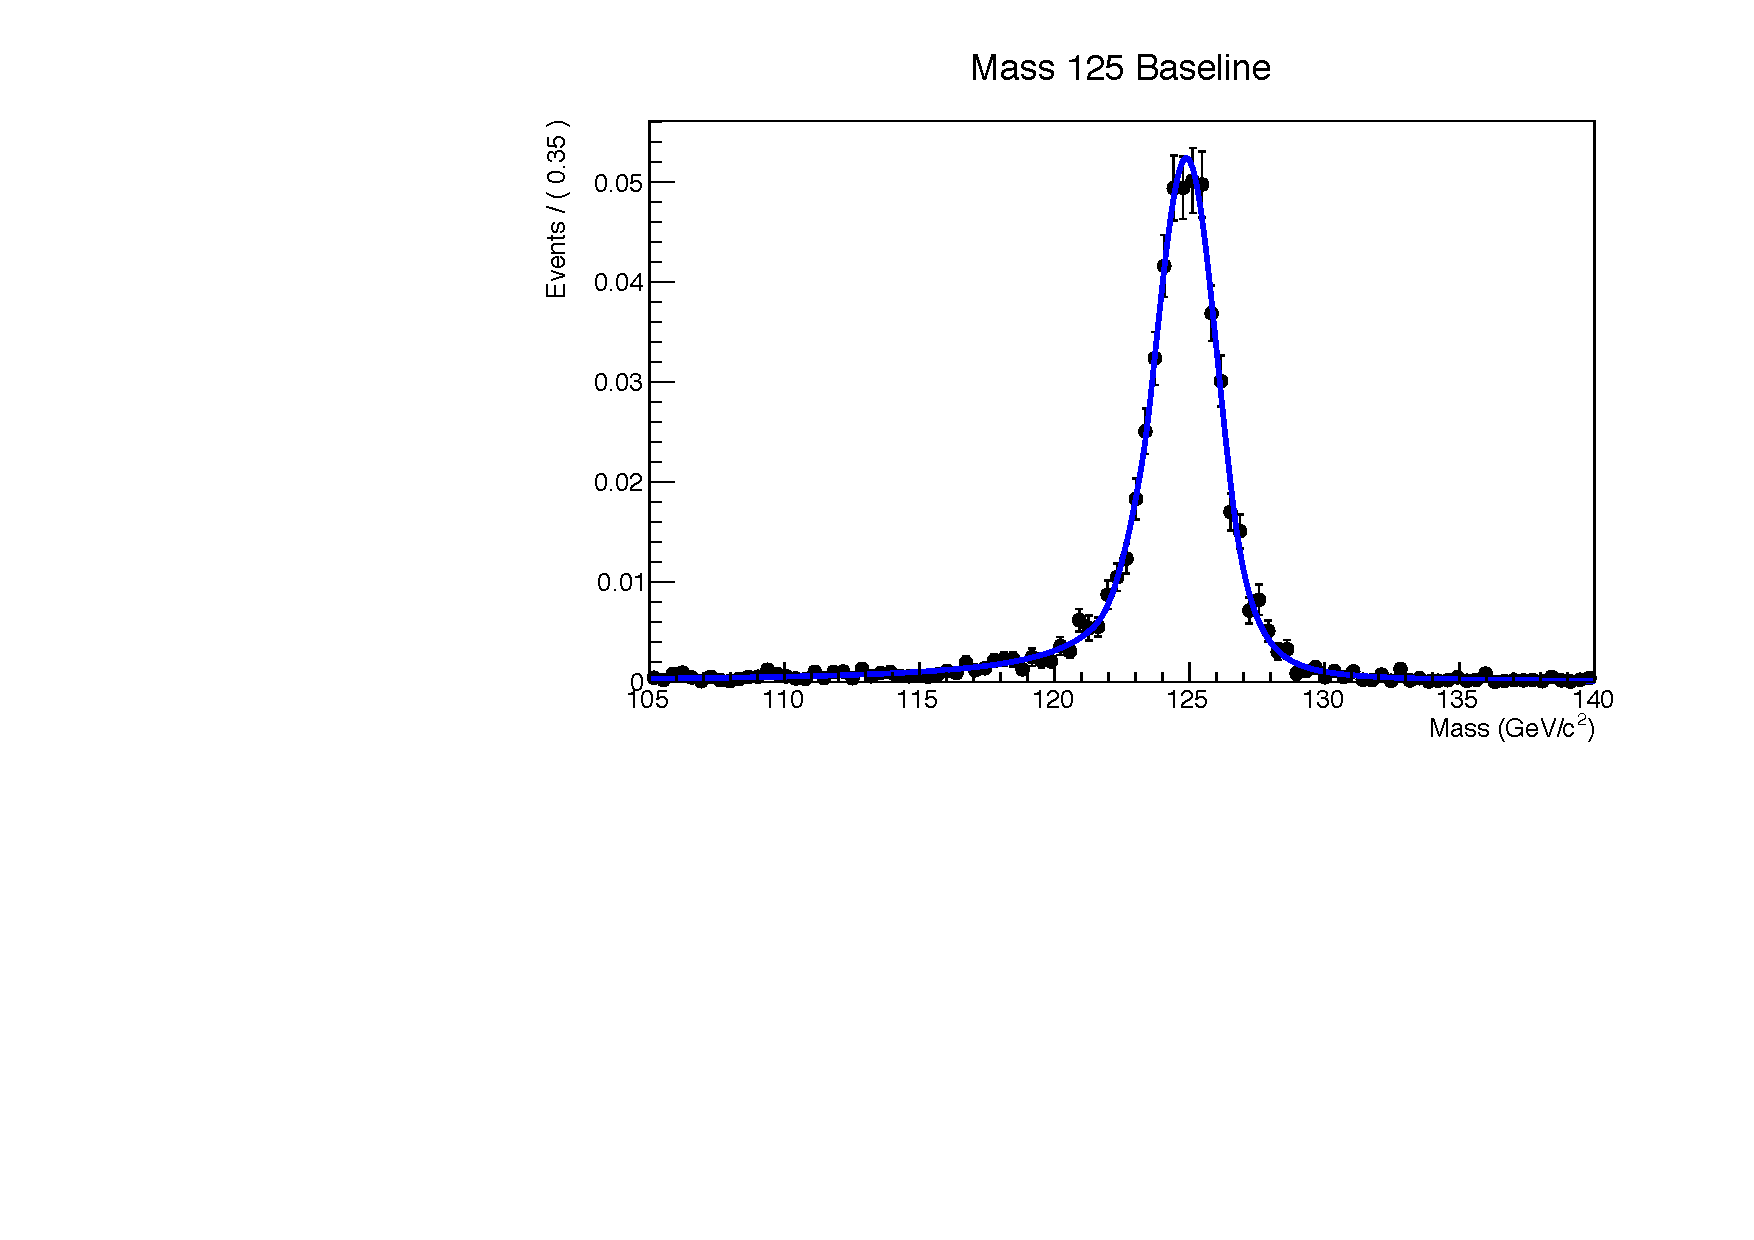
\includegraphics[width=0.3\textwidth]{Figures/SignalModelling/Signal_Parametrization/2017/WH_4mu_2017_125.pdf} 
%%		\includegraphics[width=0.3\textwidth]{Figures/SignalModelling/Signal_Parametrization/2017/2017_ZH_yield.pdf}
%		\caption{125 GeV fit in 2017: 4e ggF on the left, 
%		4$\mu$ WH on the right.}
%	\label{signal_lineshape_2017}
%	\end{center}
%\end{figure}
%\begin{figure}[!htbp]
%	\begin{center}
%   		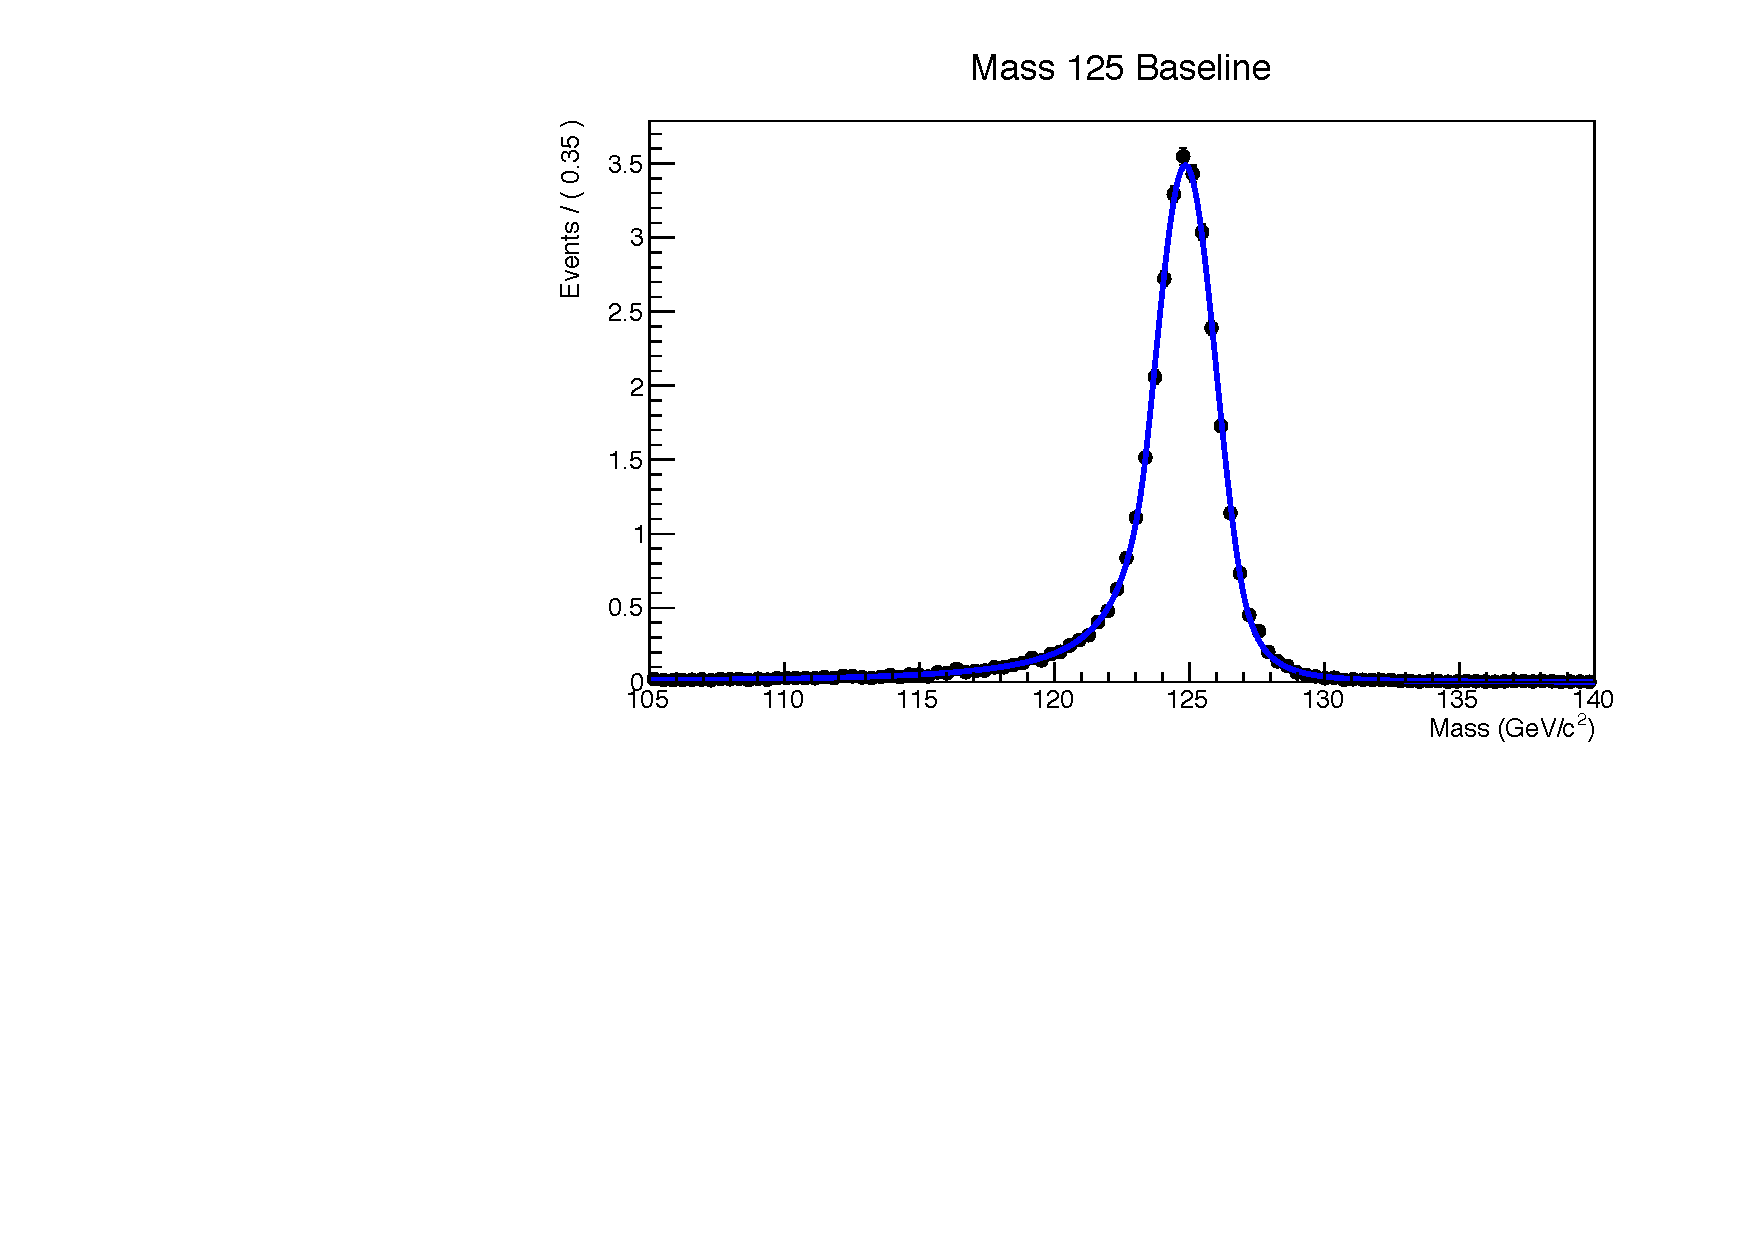
\includegraphics[width=0.3\textwidth]{Figures/SignalModelling/Signal_Parametrization/2018/ggH_4mu_2018_125.pdf}
%		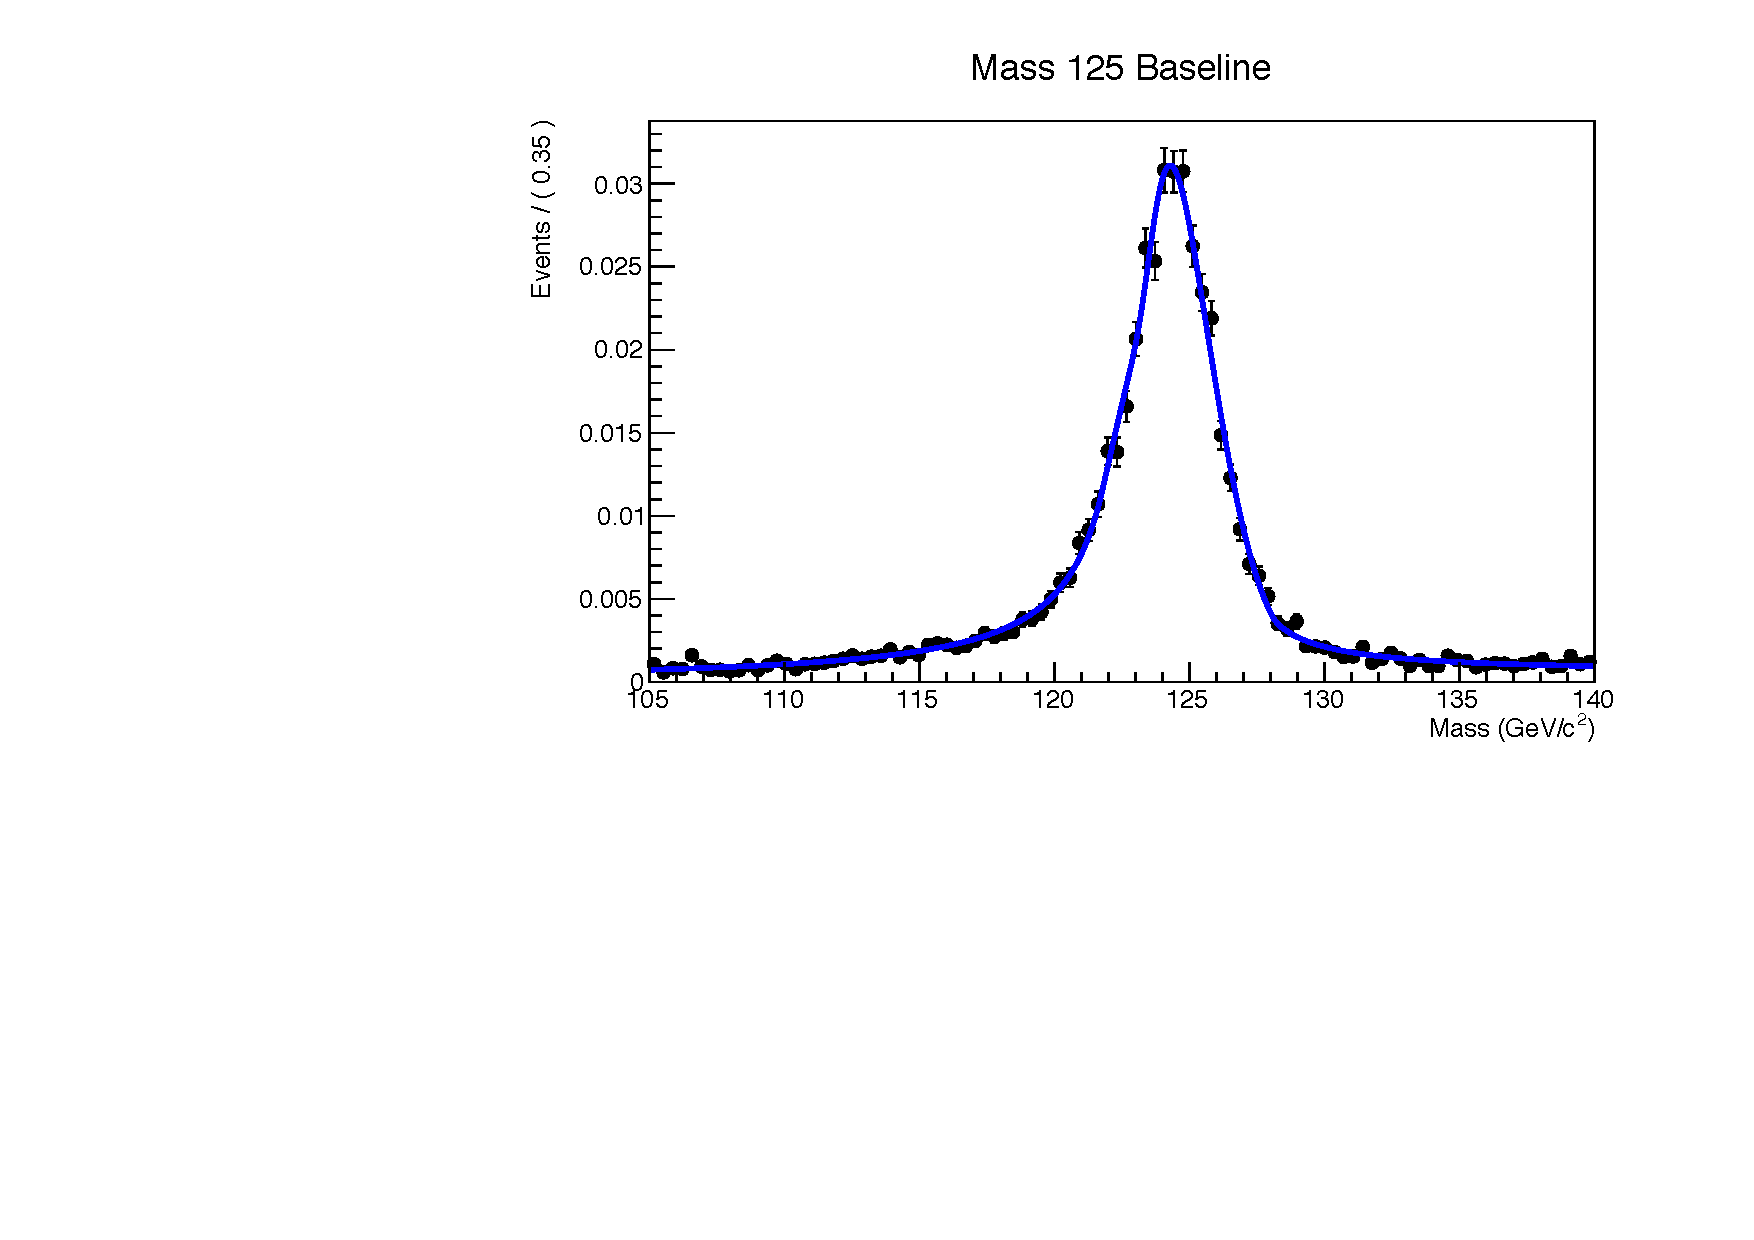
\includegraphics[width=0.3\textwidth]{Figures/SignalModelling/Signal_Parametrization/2018/ttH_2e2mu_2018_125.pdf} 
%%		\includegraphics[width=0.3\textwidth]{Figures/SignalModelling/Signal_Parametrization/2017/2018_ttH_yield.pdf}
%		\caption{125 GeV fit in 2018: 4$\mu$ ggF on the left, 
%		2e2$\mu$ ttH on the right.}
%	\label{signal_lineshape_2018}
%	\end{center}
%\end{figure}
%
%
%\begin{figure}[!htbp]
%	\begin{center}
%   		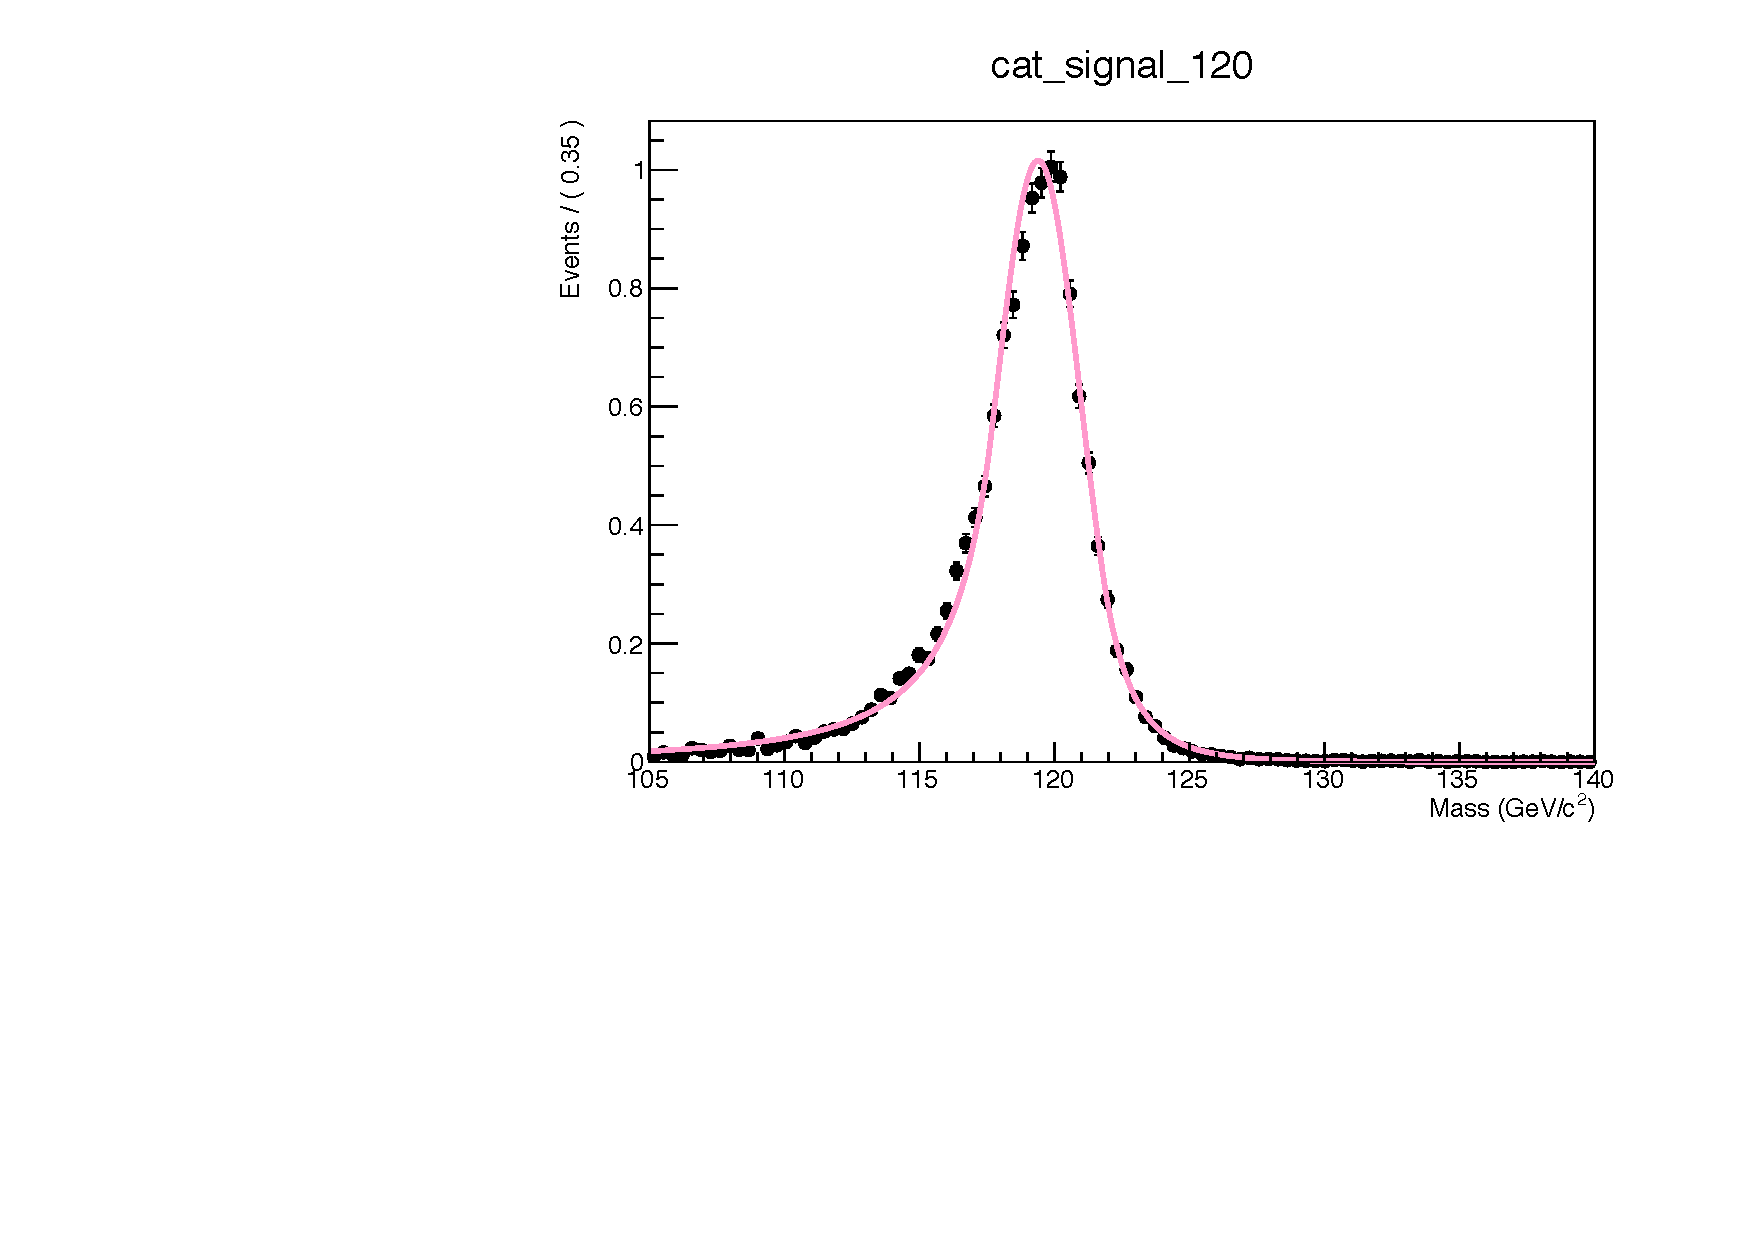
\includegraphics[width=0.3\textwidth]{Figures/SignalModelling/Signal_Parametrization/2016/ggH_2e2mu_2016_120_Sim.pdf}
%	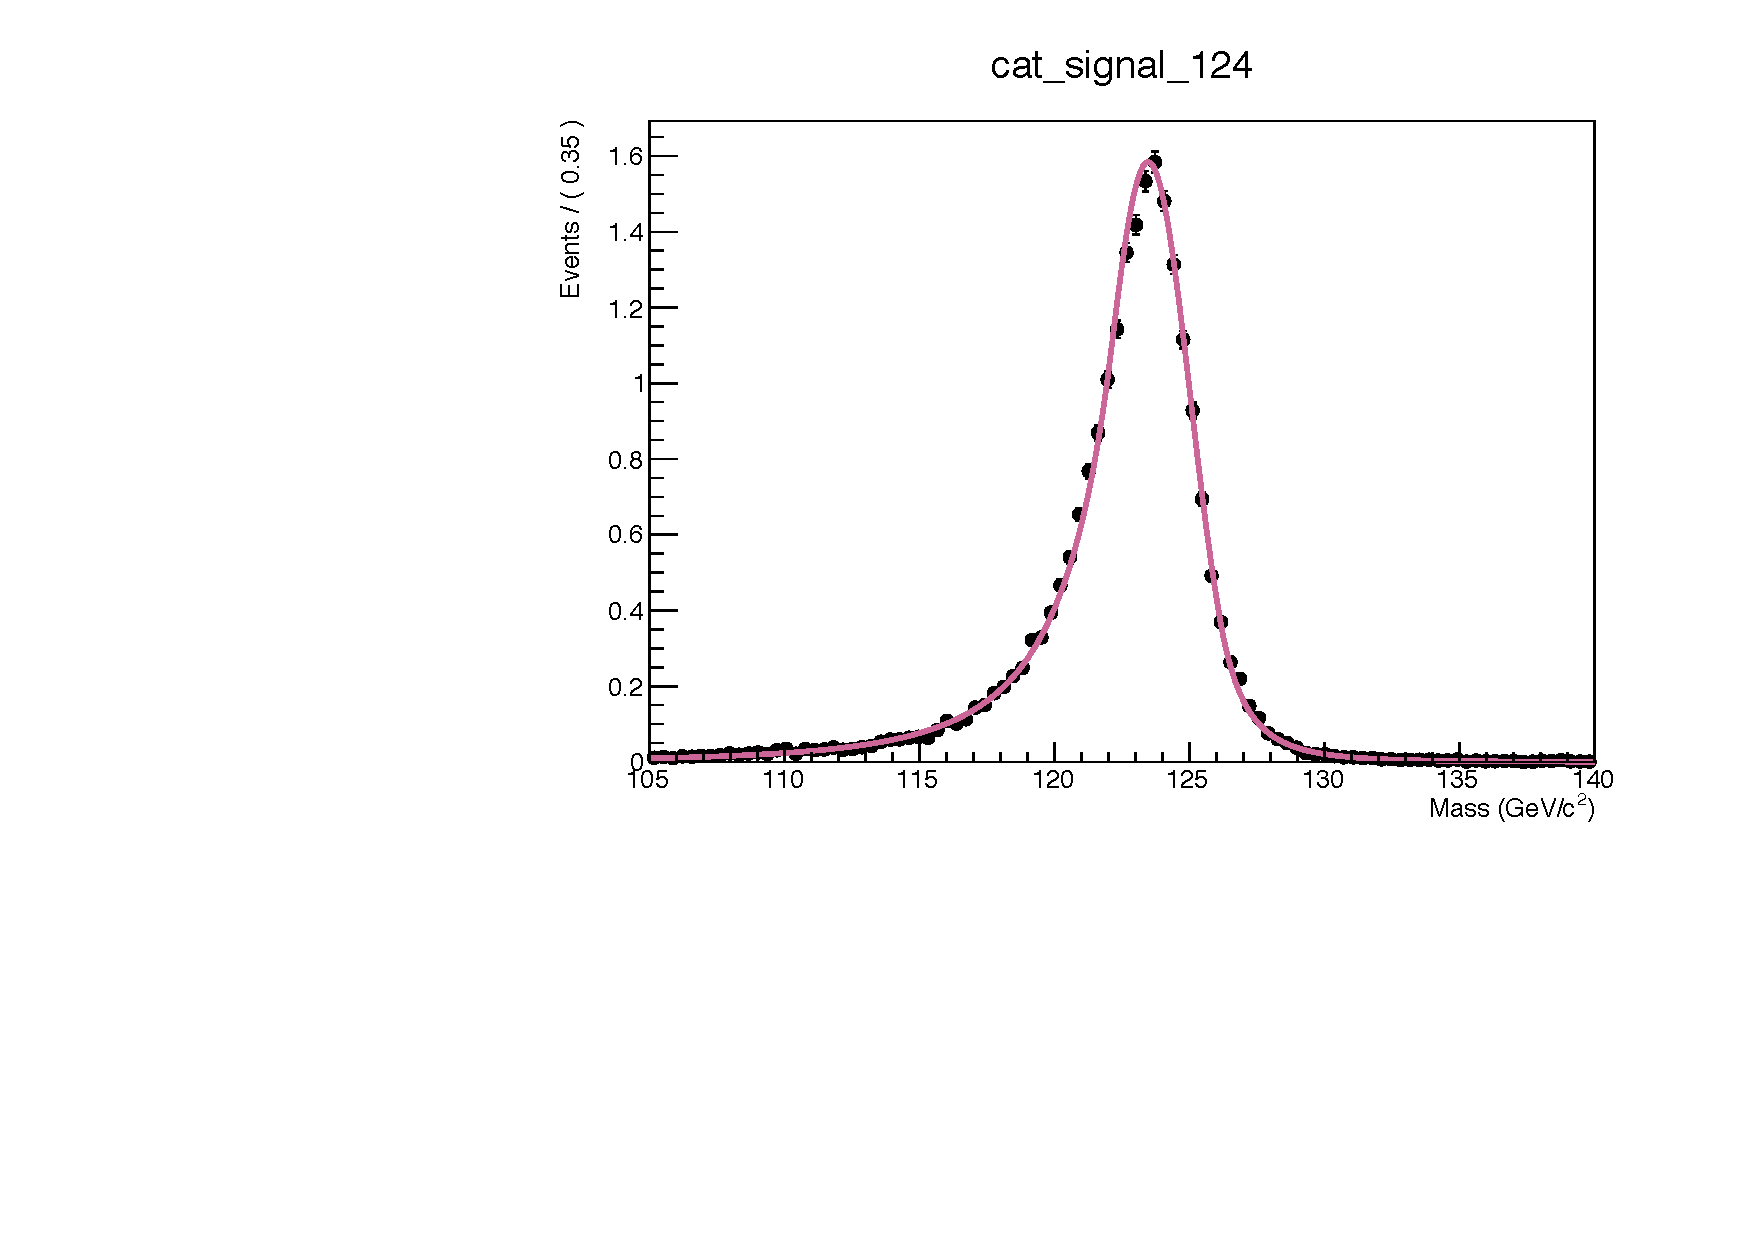
\includegraphics[width=0.3\textwidth]{Figures/SignalModelling/Signal_Parametrization/2016/ggH_2e2mu_2016_124_Sim.pdf} 
%	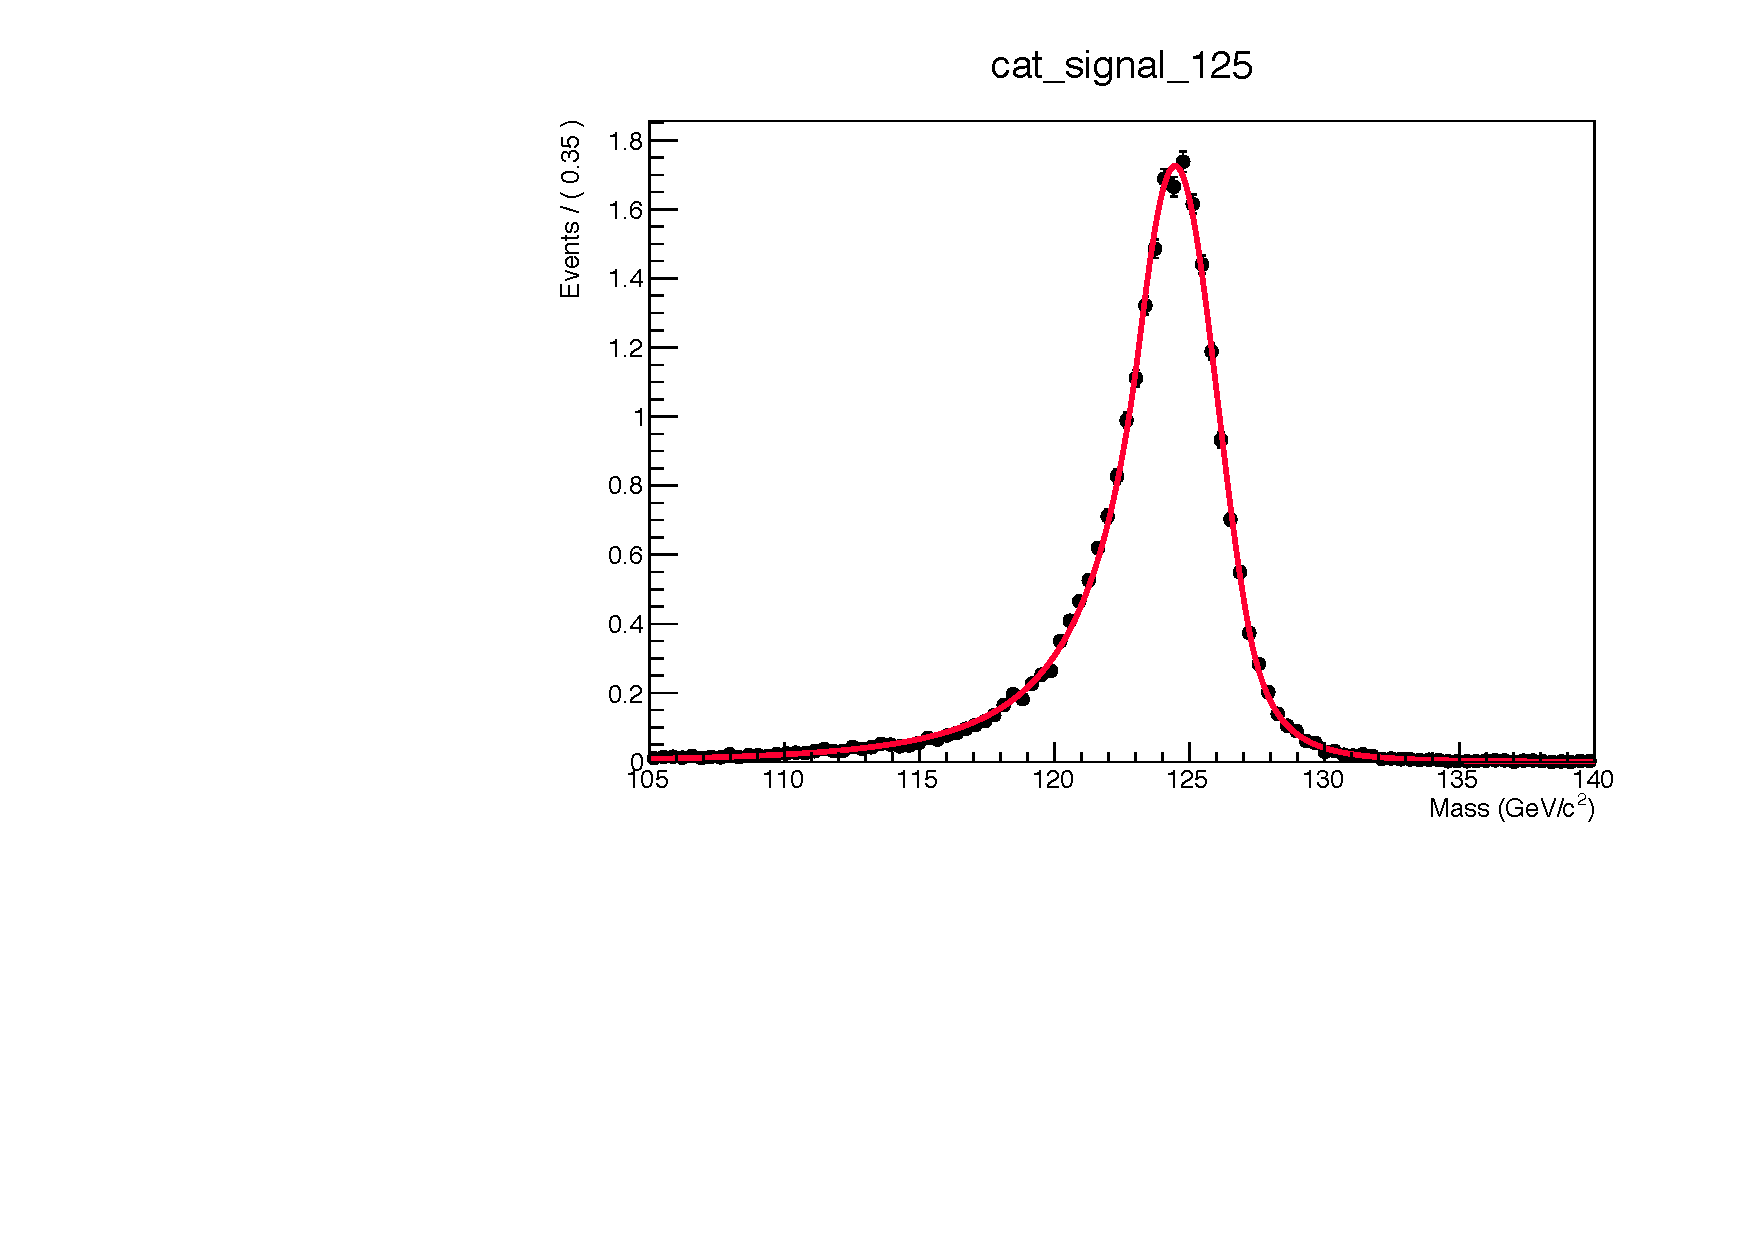
\includegraphics[width=0.3\textwidth]{Figures/SignalModelling/Signal_Parametrization/2016/ggH_2e2mu_2016_125_Sim.pdf}
%		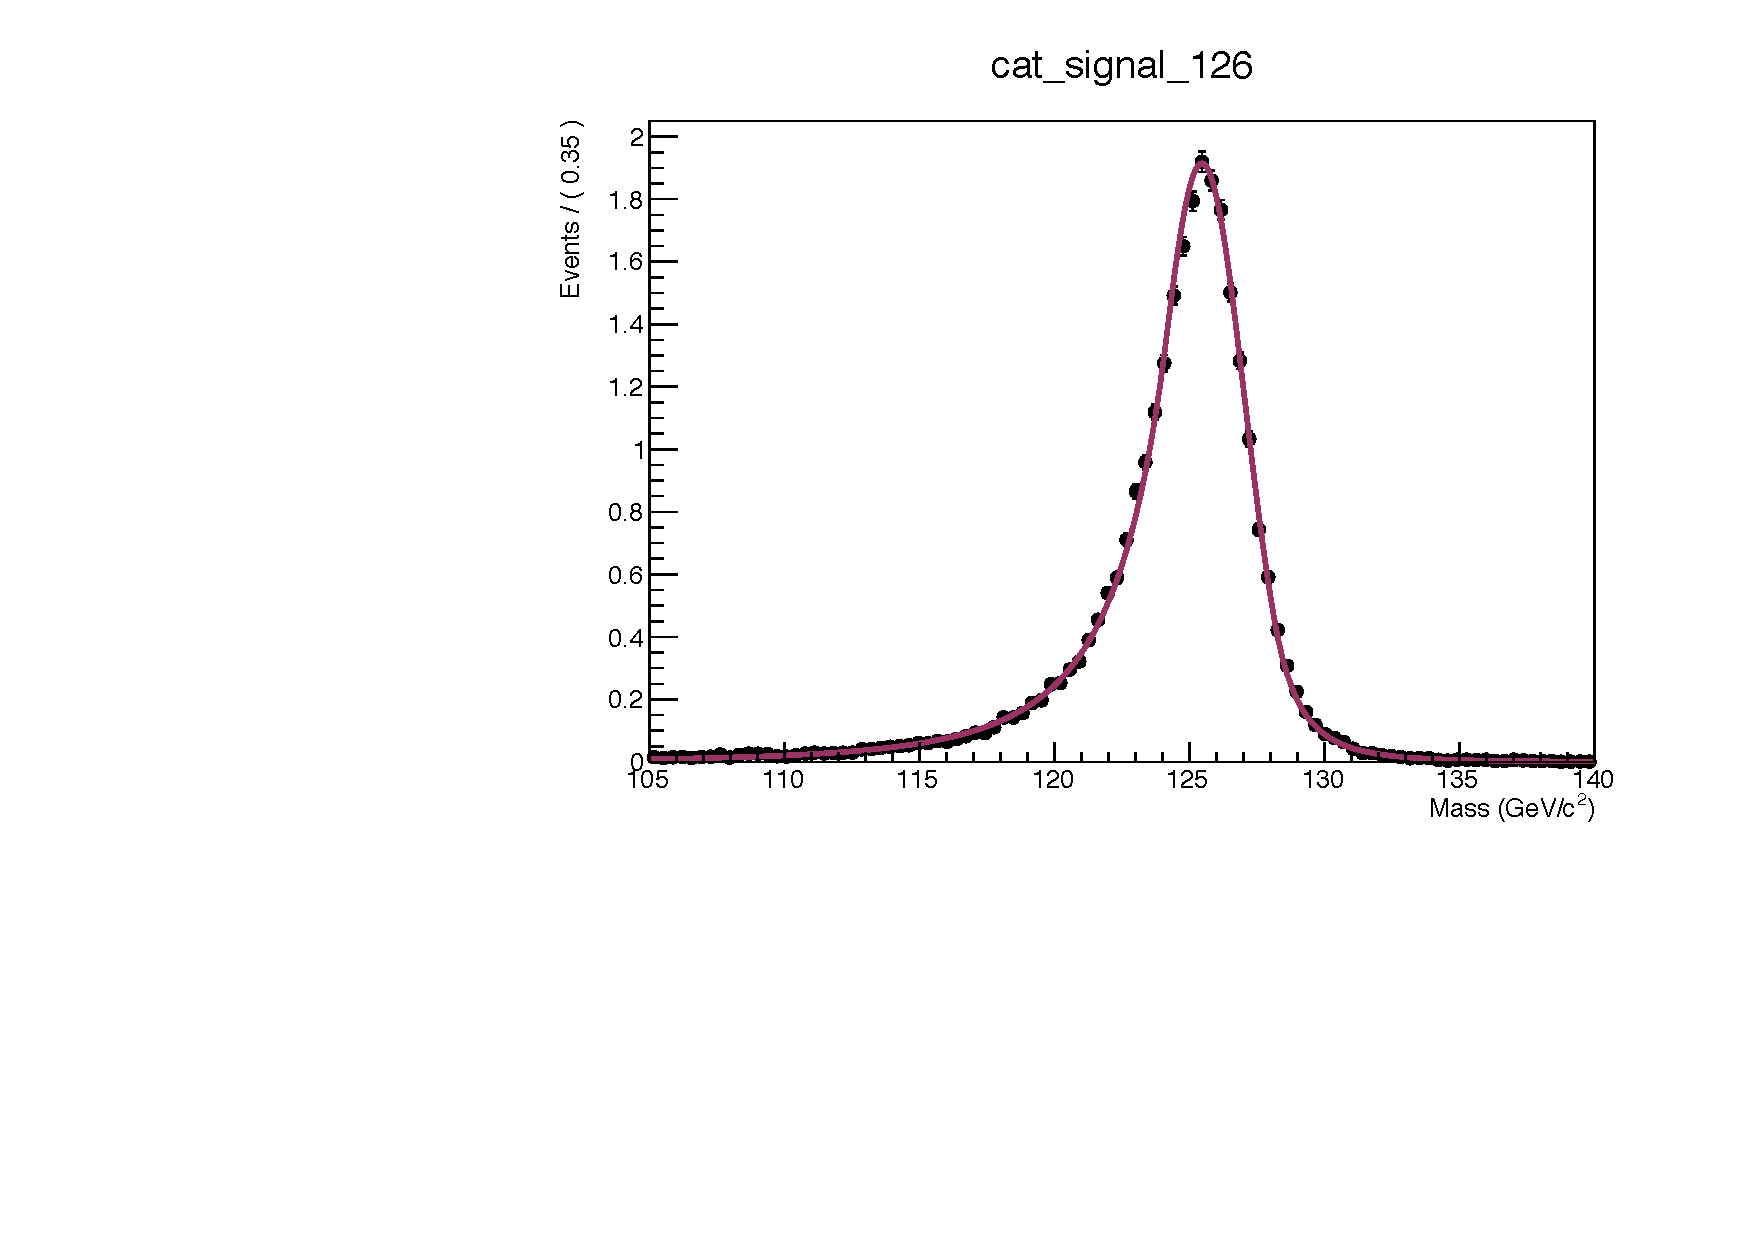
\includegraphics[width=0.3\textwidth]{Figures/SignalModelling/Signal_Parametrization/2016/ggH_2e2mu_2016_126_Sim.pdf}
%		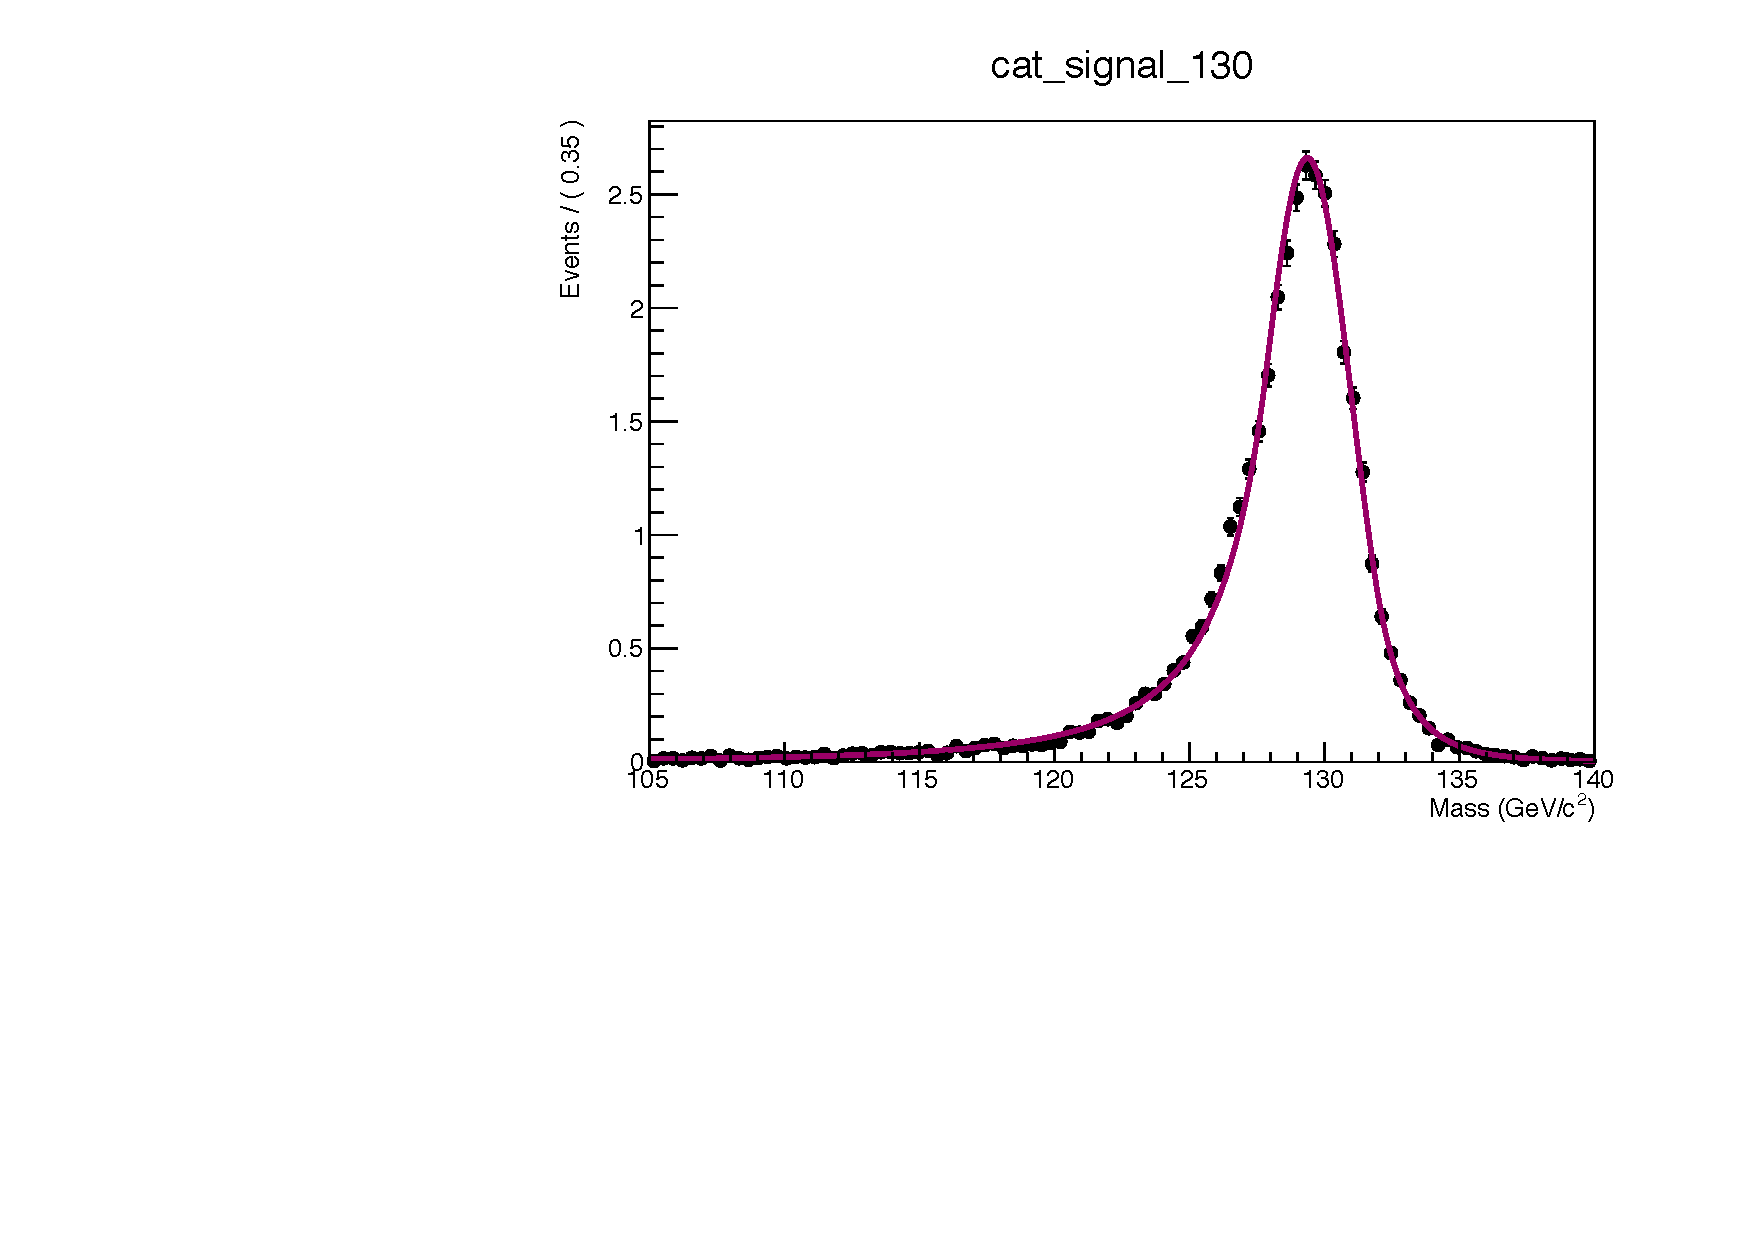
\includegraphics[width=0.3\textwidth]{Figures/SignalModelling/Signal_Parametrization/2016/ggH_2e2mu_2016_130_Sim.pdf}
%		\caption{Simultaneous fit for ggH production mode, in 2016, for different mass points, 
%		in 2e2$\mu$ final state.}
%	\label{signal_lineshape_2016_full_1}
%	\end{center}
%\end{figure}
%\begin{figure}[!htbp]
%	\begin{center}
%   		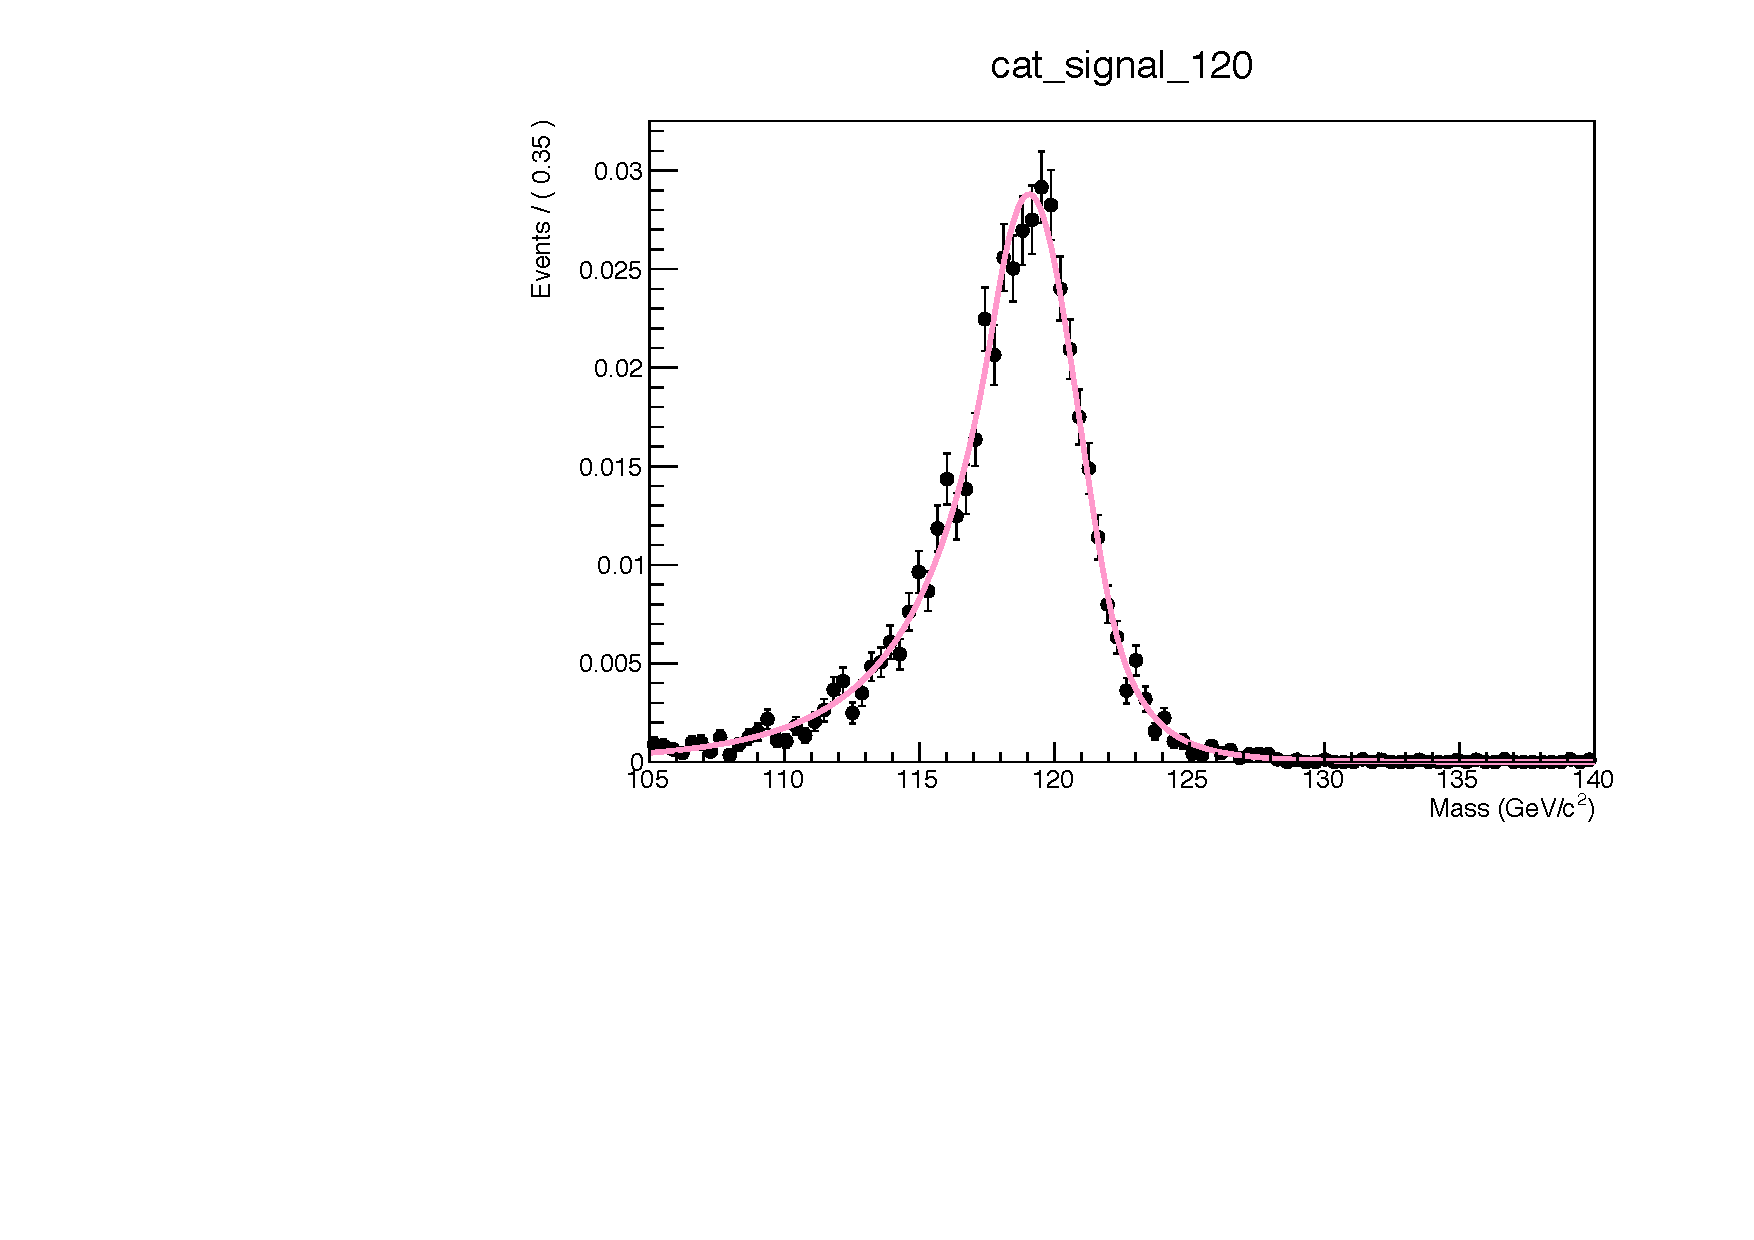
\includegraphics[width=0.3\textwidth]{Figures/SignalModelling/Signal_Parametrization/2016/VBF_4e_2016_120_Sim.pdf}
%		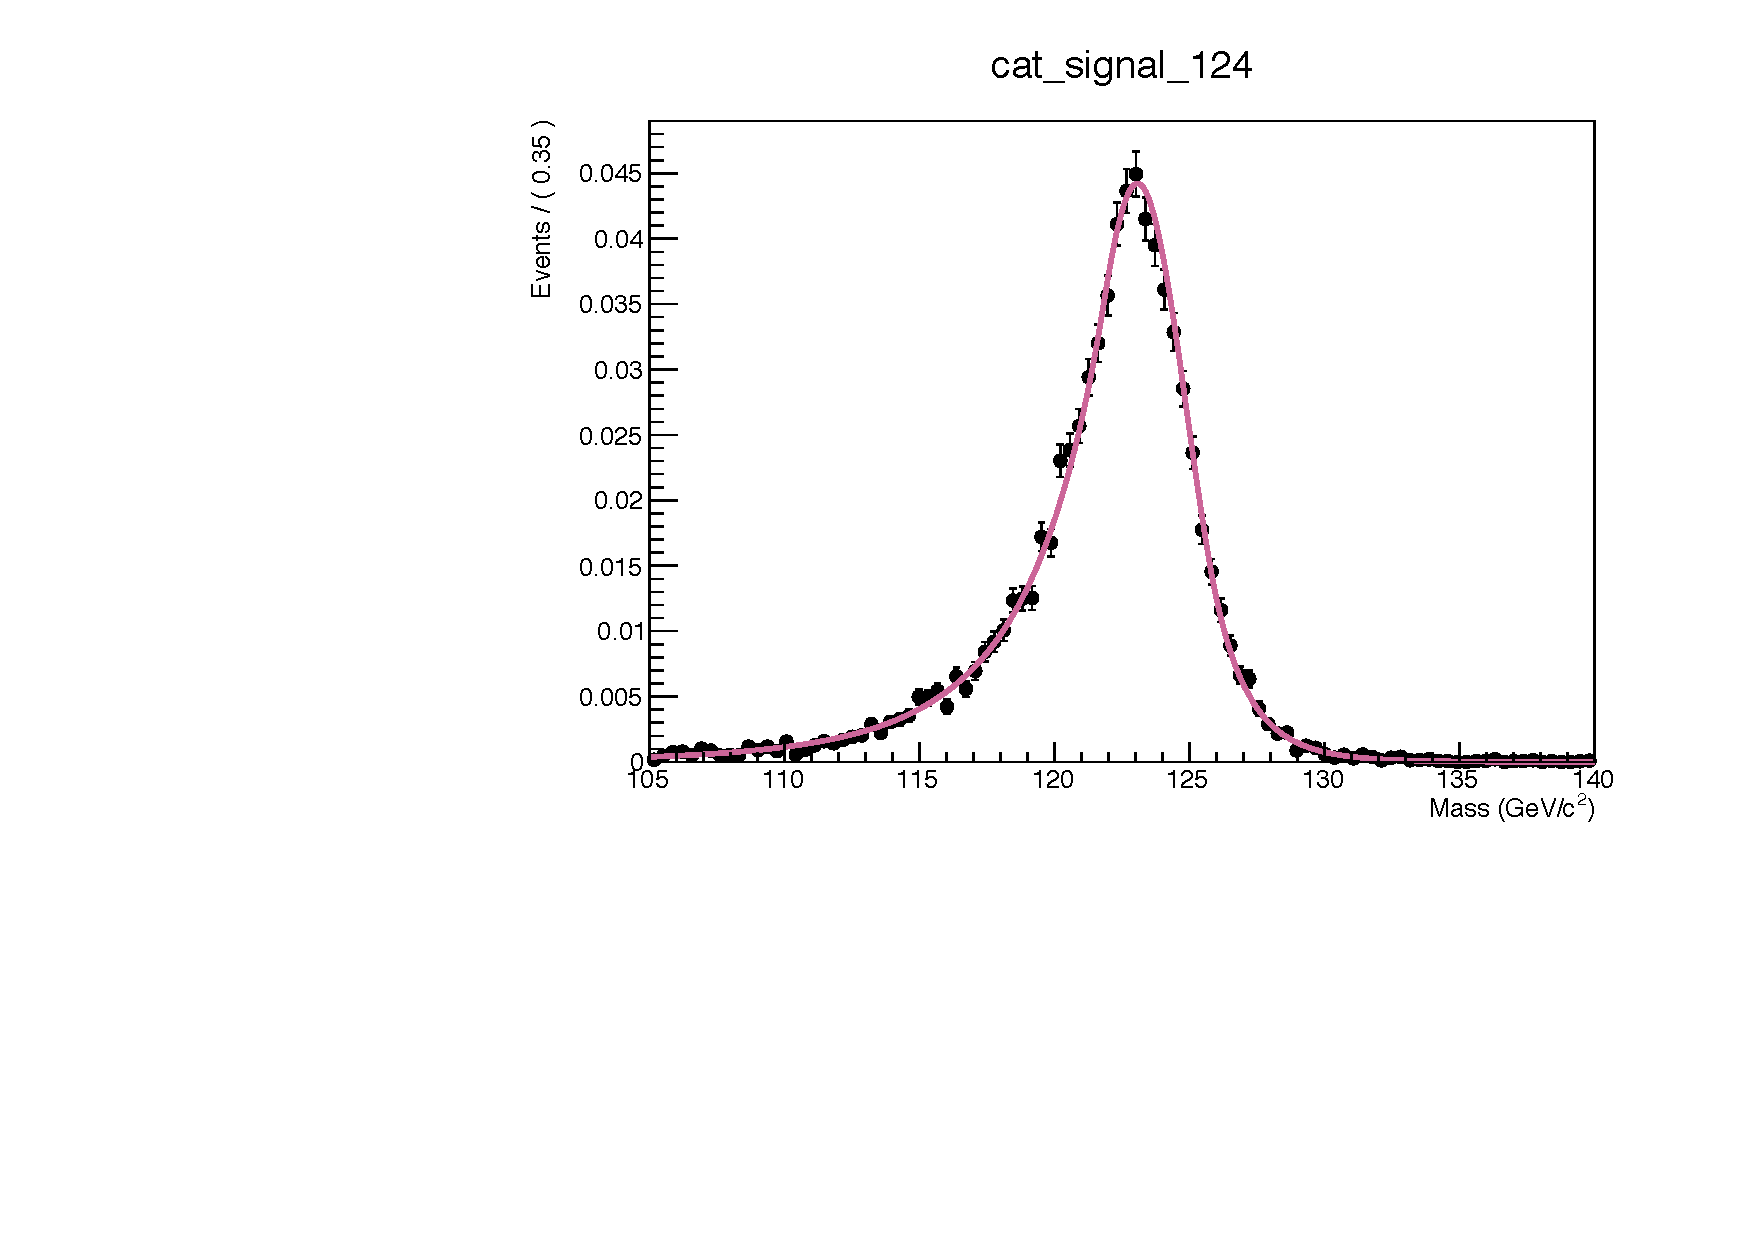
\includegraphics[width=0.3\textwidth]{Figures/SignalModelling/Signal_Parametrization/2016/VBF_4e_2016_124_Sim.pdf} 
%		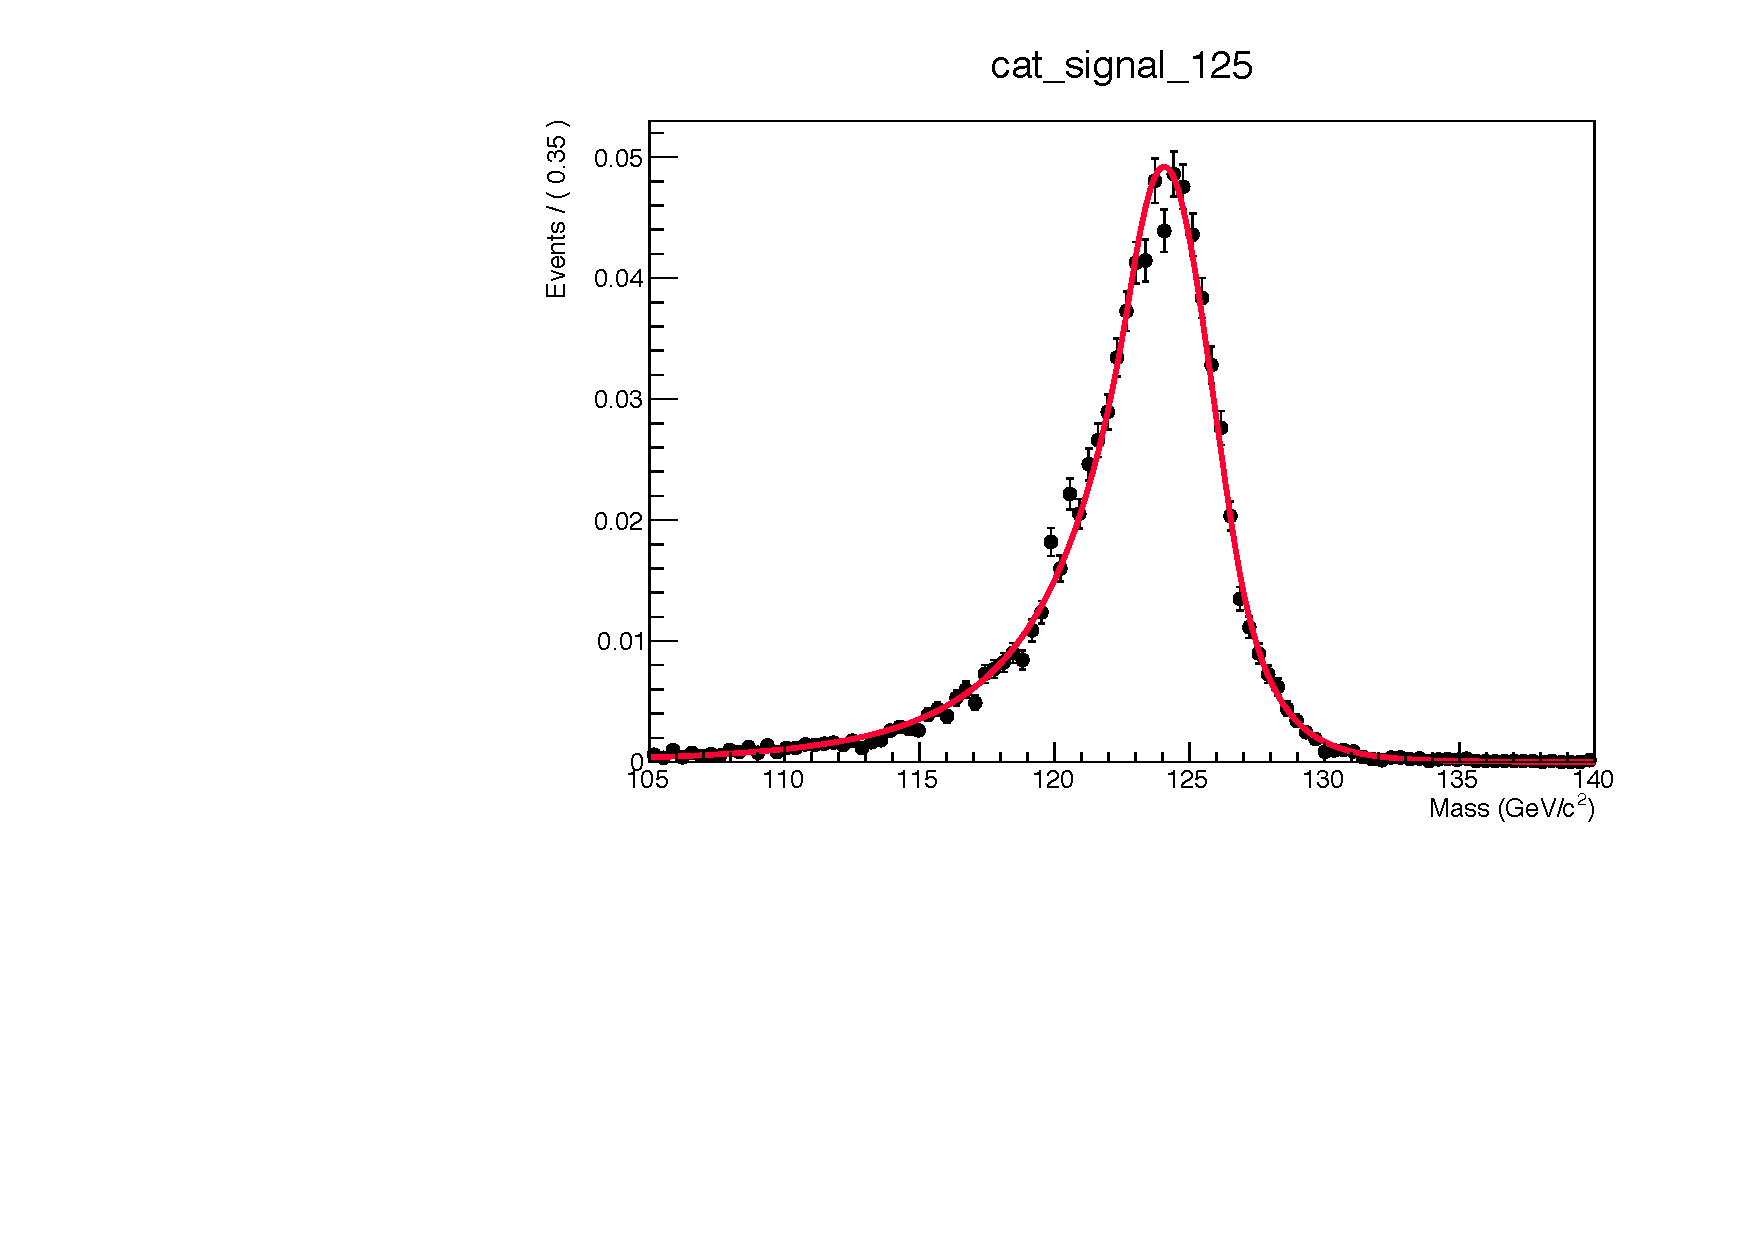
\includegraphics[width=0.3\textwidth]{Figures/SignalModelling/Signal_Parametrization/2016/VBF_4e_2016_125_Sim.pdf}
%		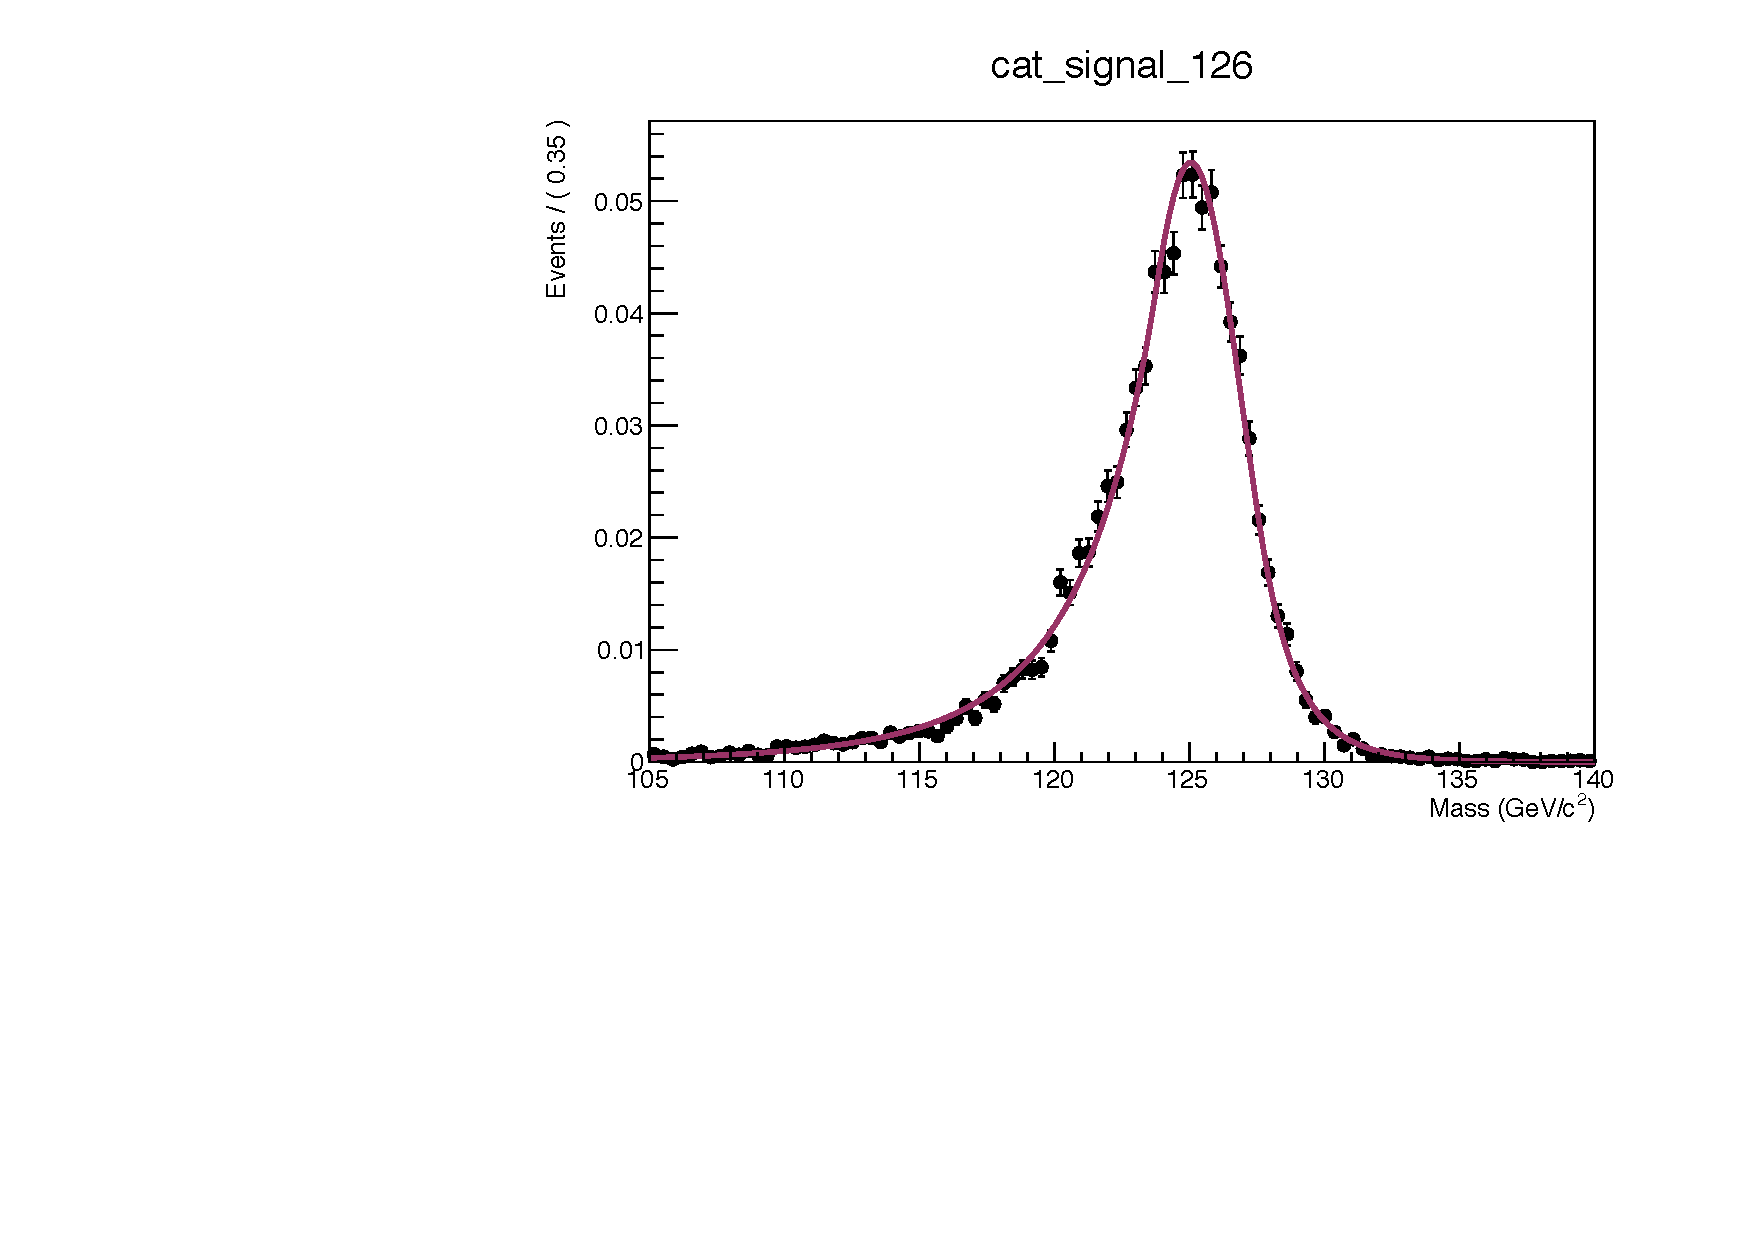
\includegraphics[width=0.3\textwidth]{Figures/SignalModelling/Signal_Parametrization/2016/VBF_4e_2016_126_Sim.pdf}
%		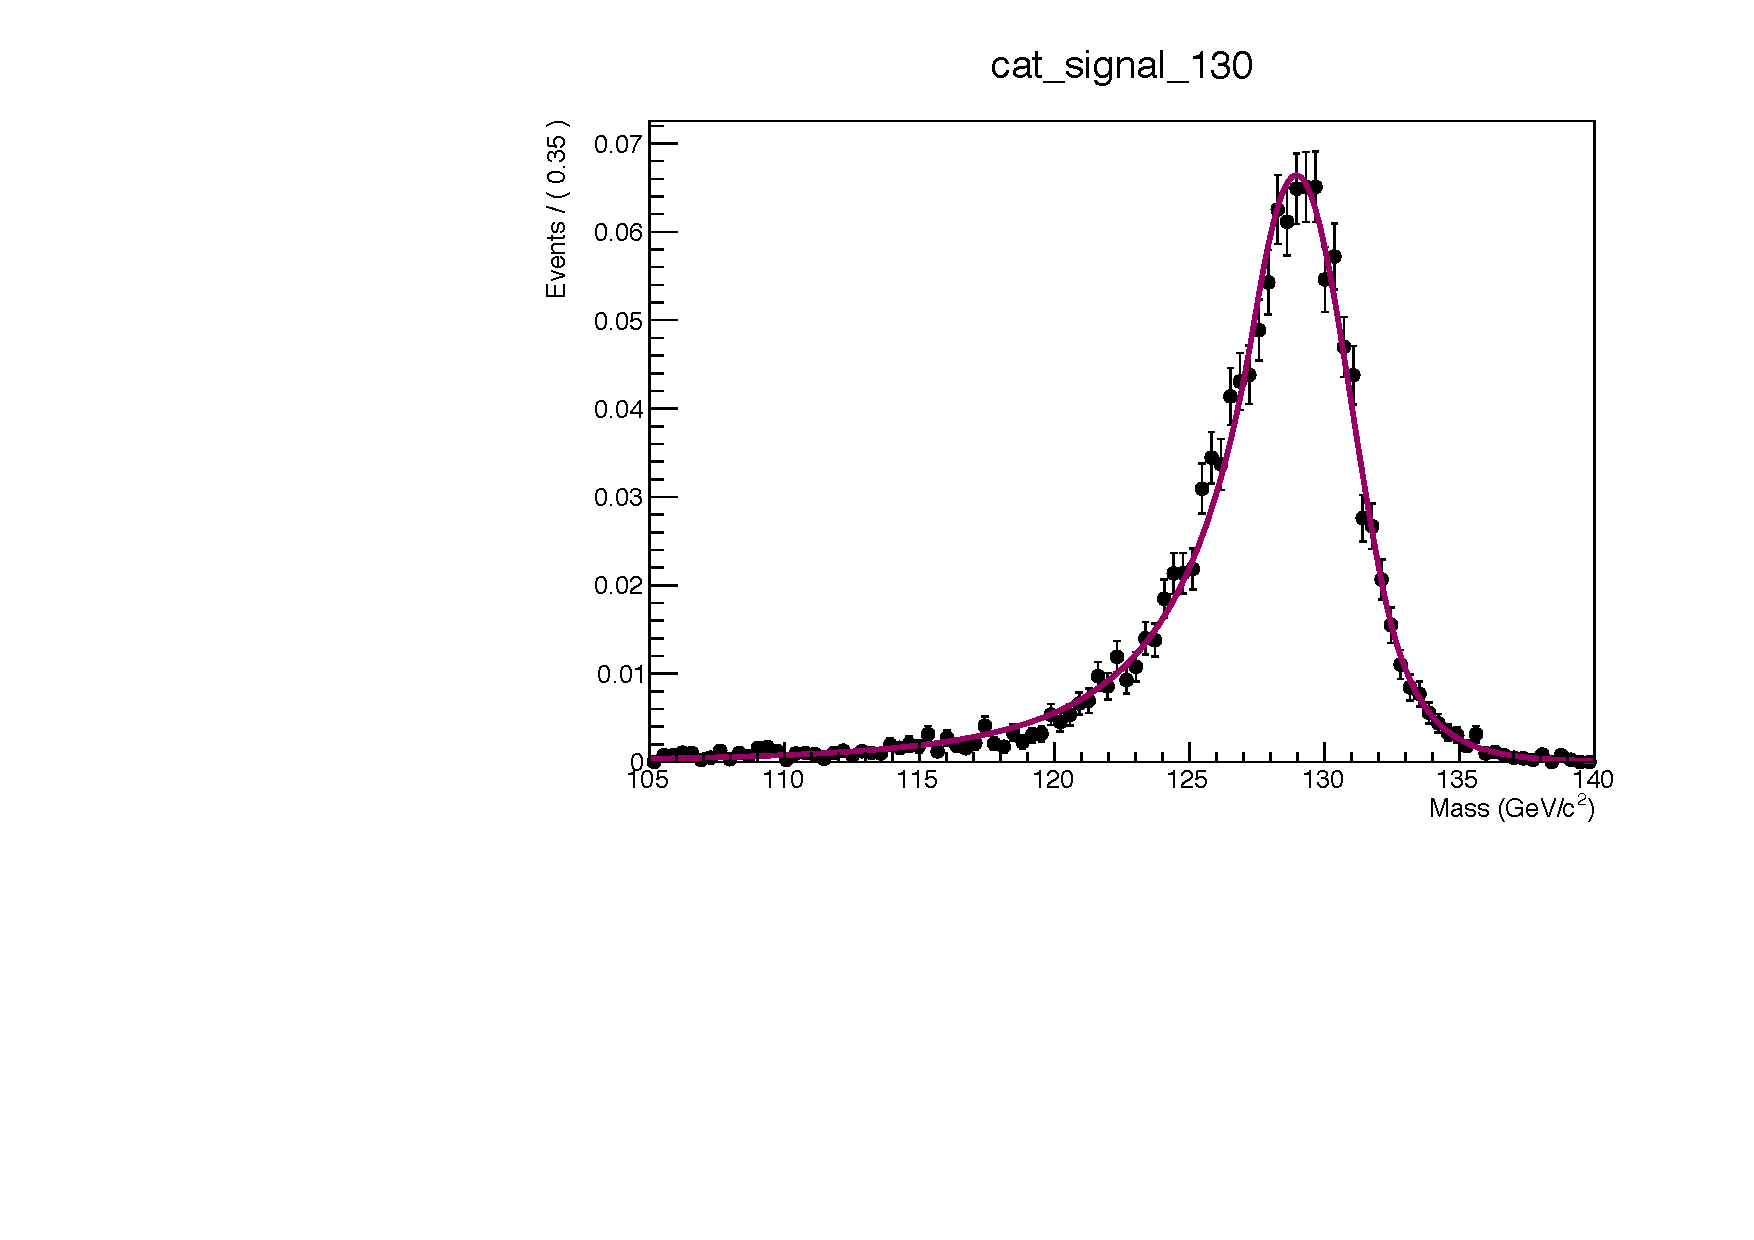
\includegraphics[width=0.3\textwidth]{Figures/SignalModelling/Signal_Parametrization/2016/VBF_4e_2016_130_Sim.pdf}
%		\caption{Simultaneous fit for VBF production mode, in 2016, for different mass points, 
%		in 4e final state.}
%	\label{signal_lineshape_2016_full_2}
%	\end{center}
%\end{figure}
%\begin{figure}[!htbp]
%	\begin{center}
%		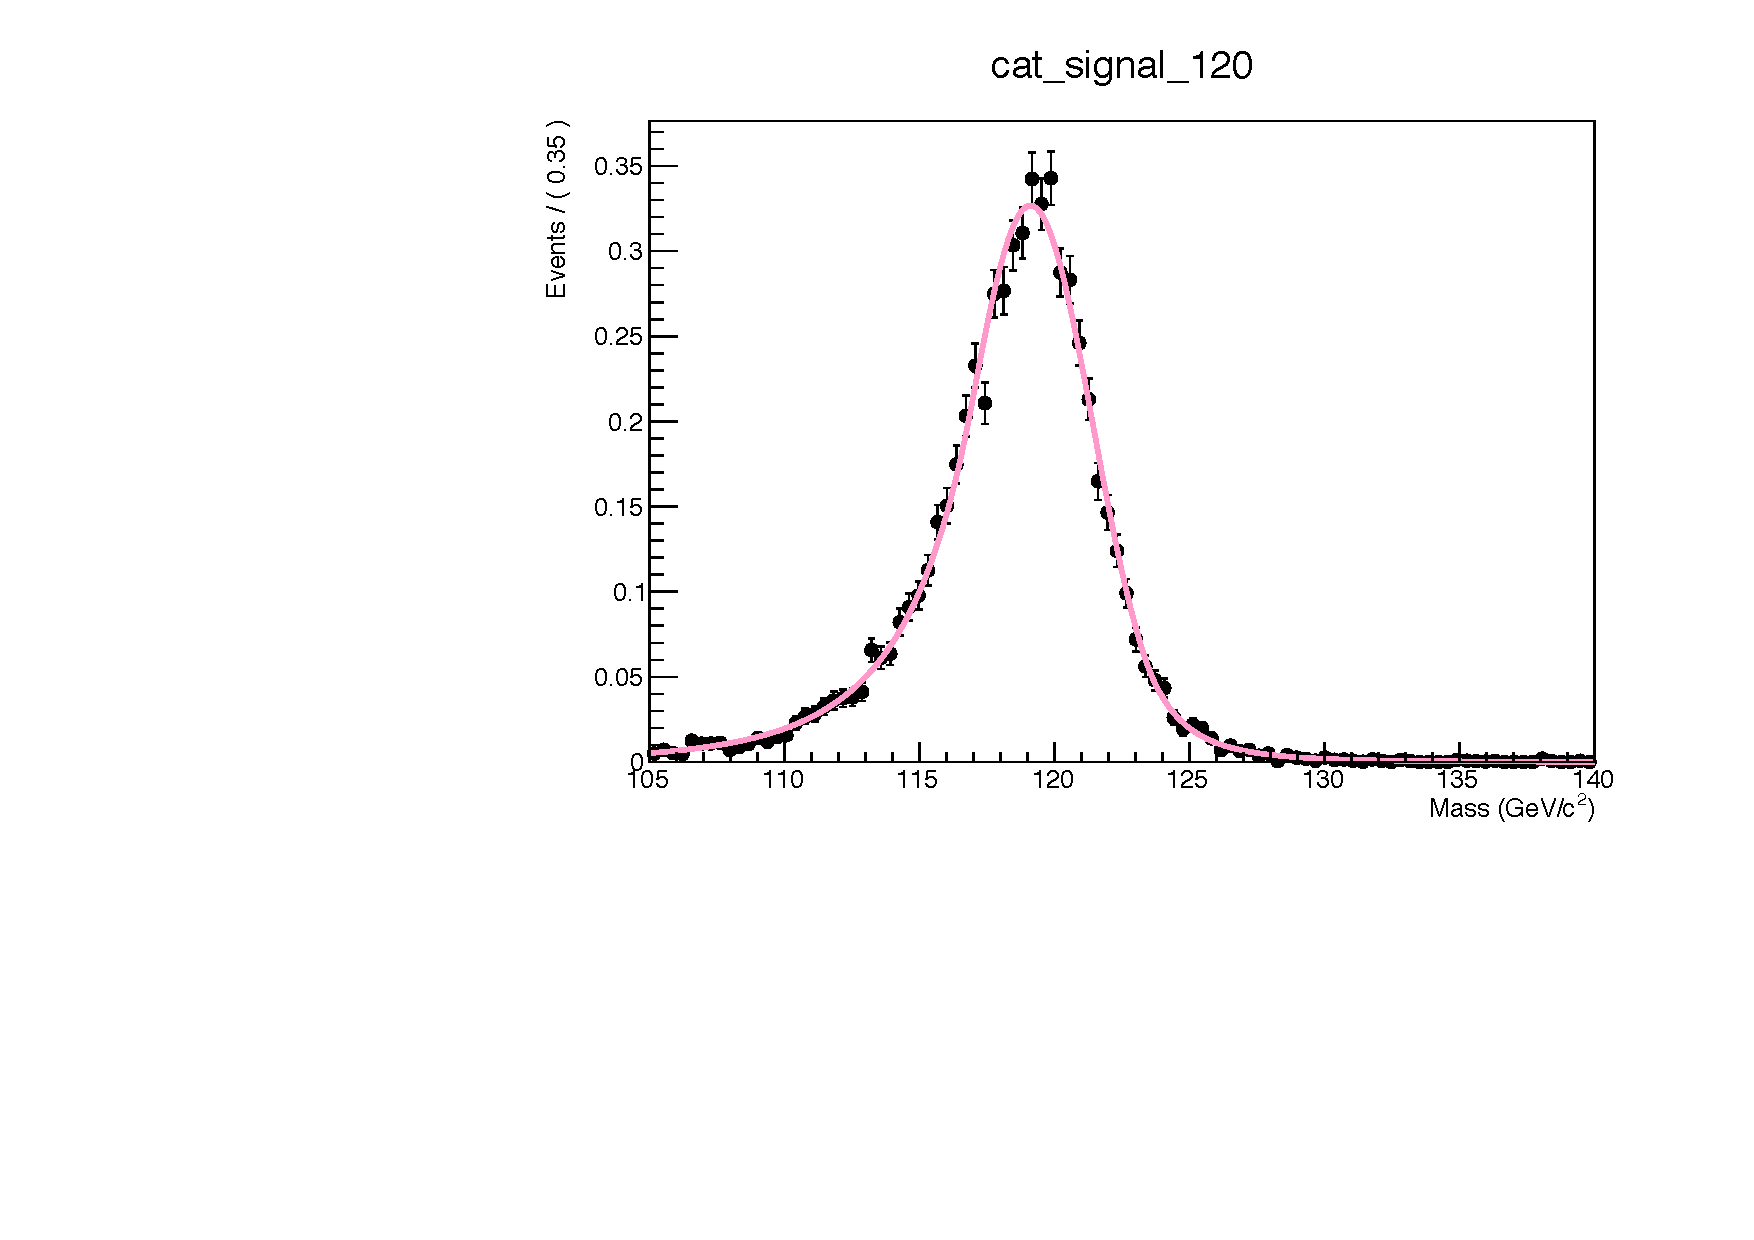
\includegraphics[width=0.3\textwidth]{Figures/SignalModelling/Signal_Parametrization/2017/ggH_4e_2017_120_Sim.pdf}
%		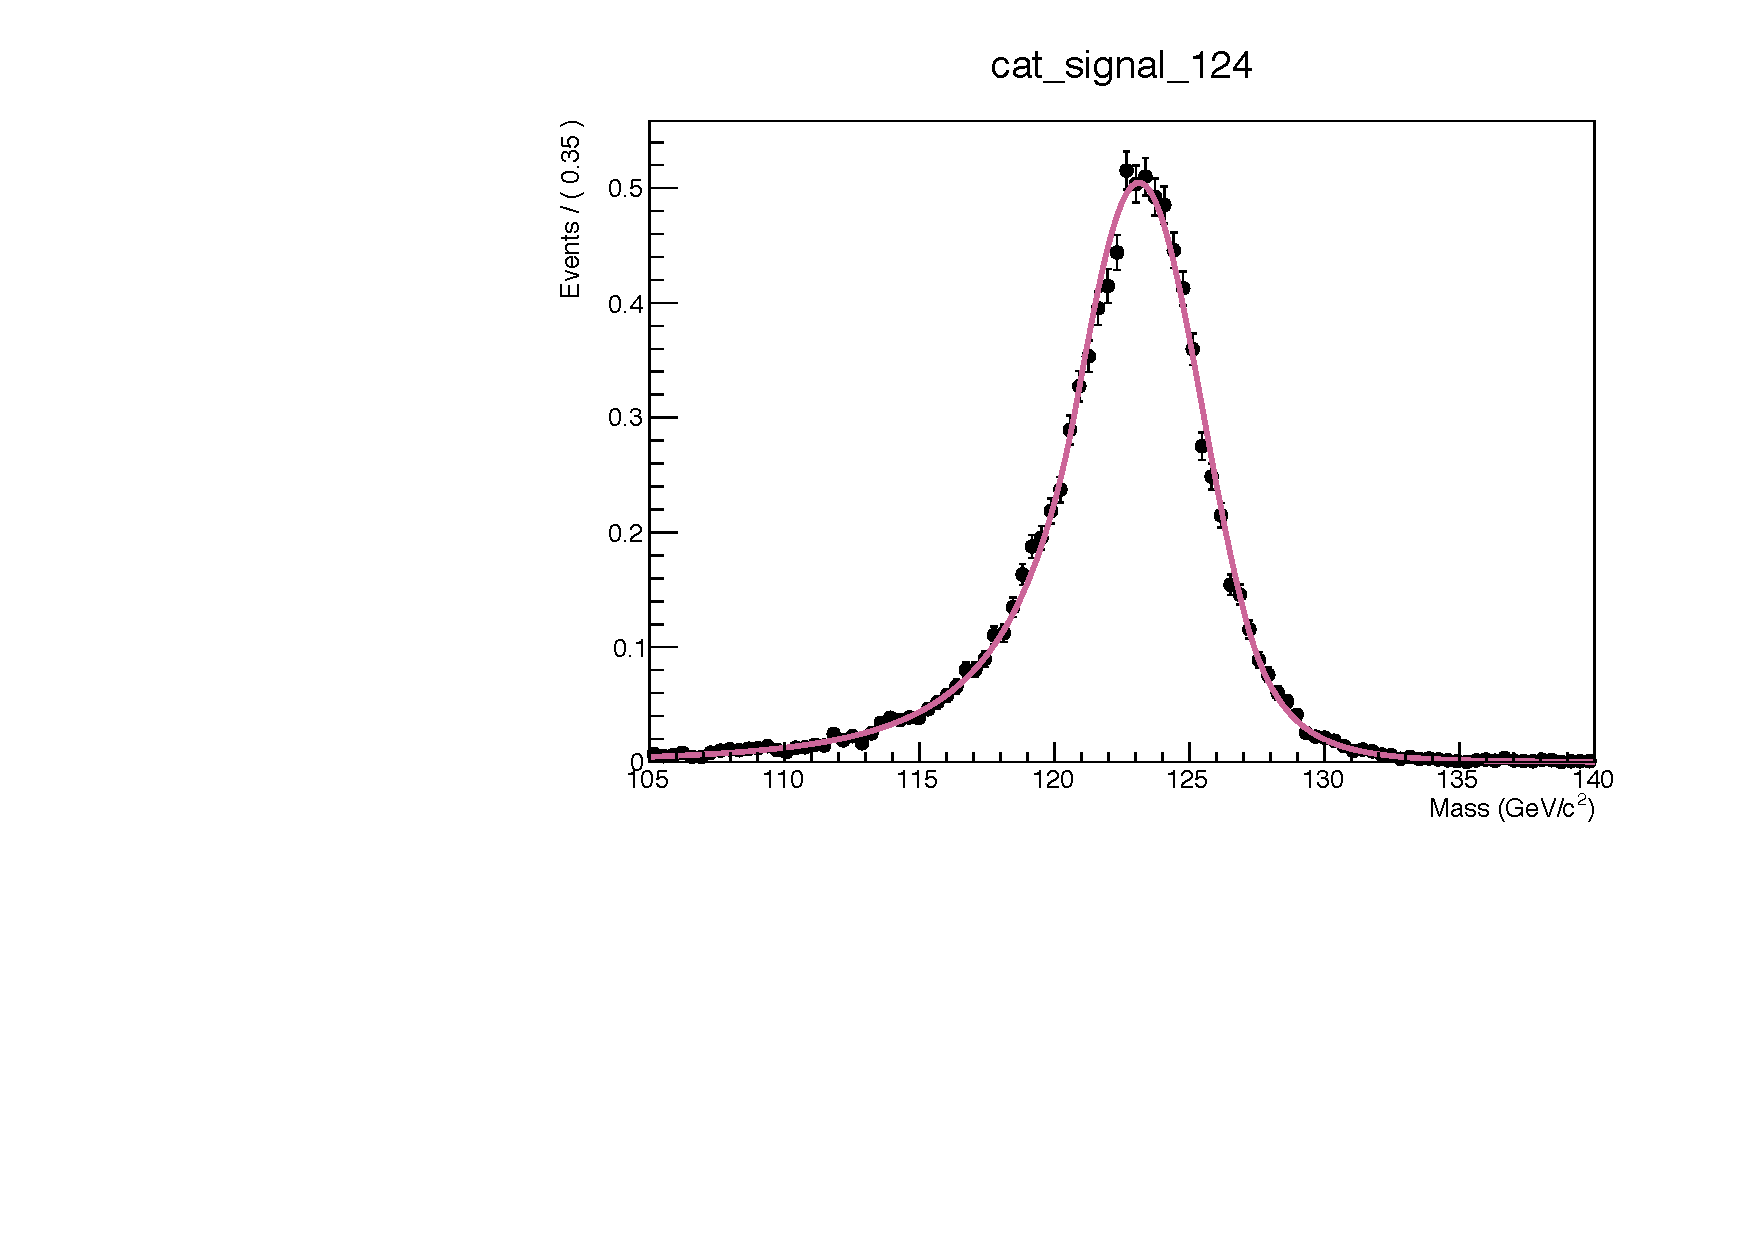
\includegraphics[width=0.3\textwidth]{Figures/SignalModelling/Signal_Parametrization/2017/ggH_4e_2017_124_Sim.pdf}
%   		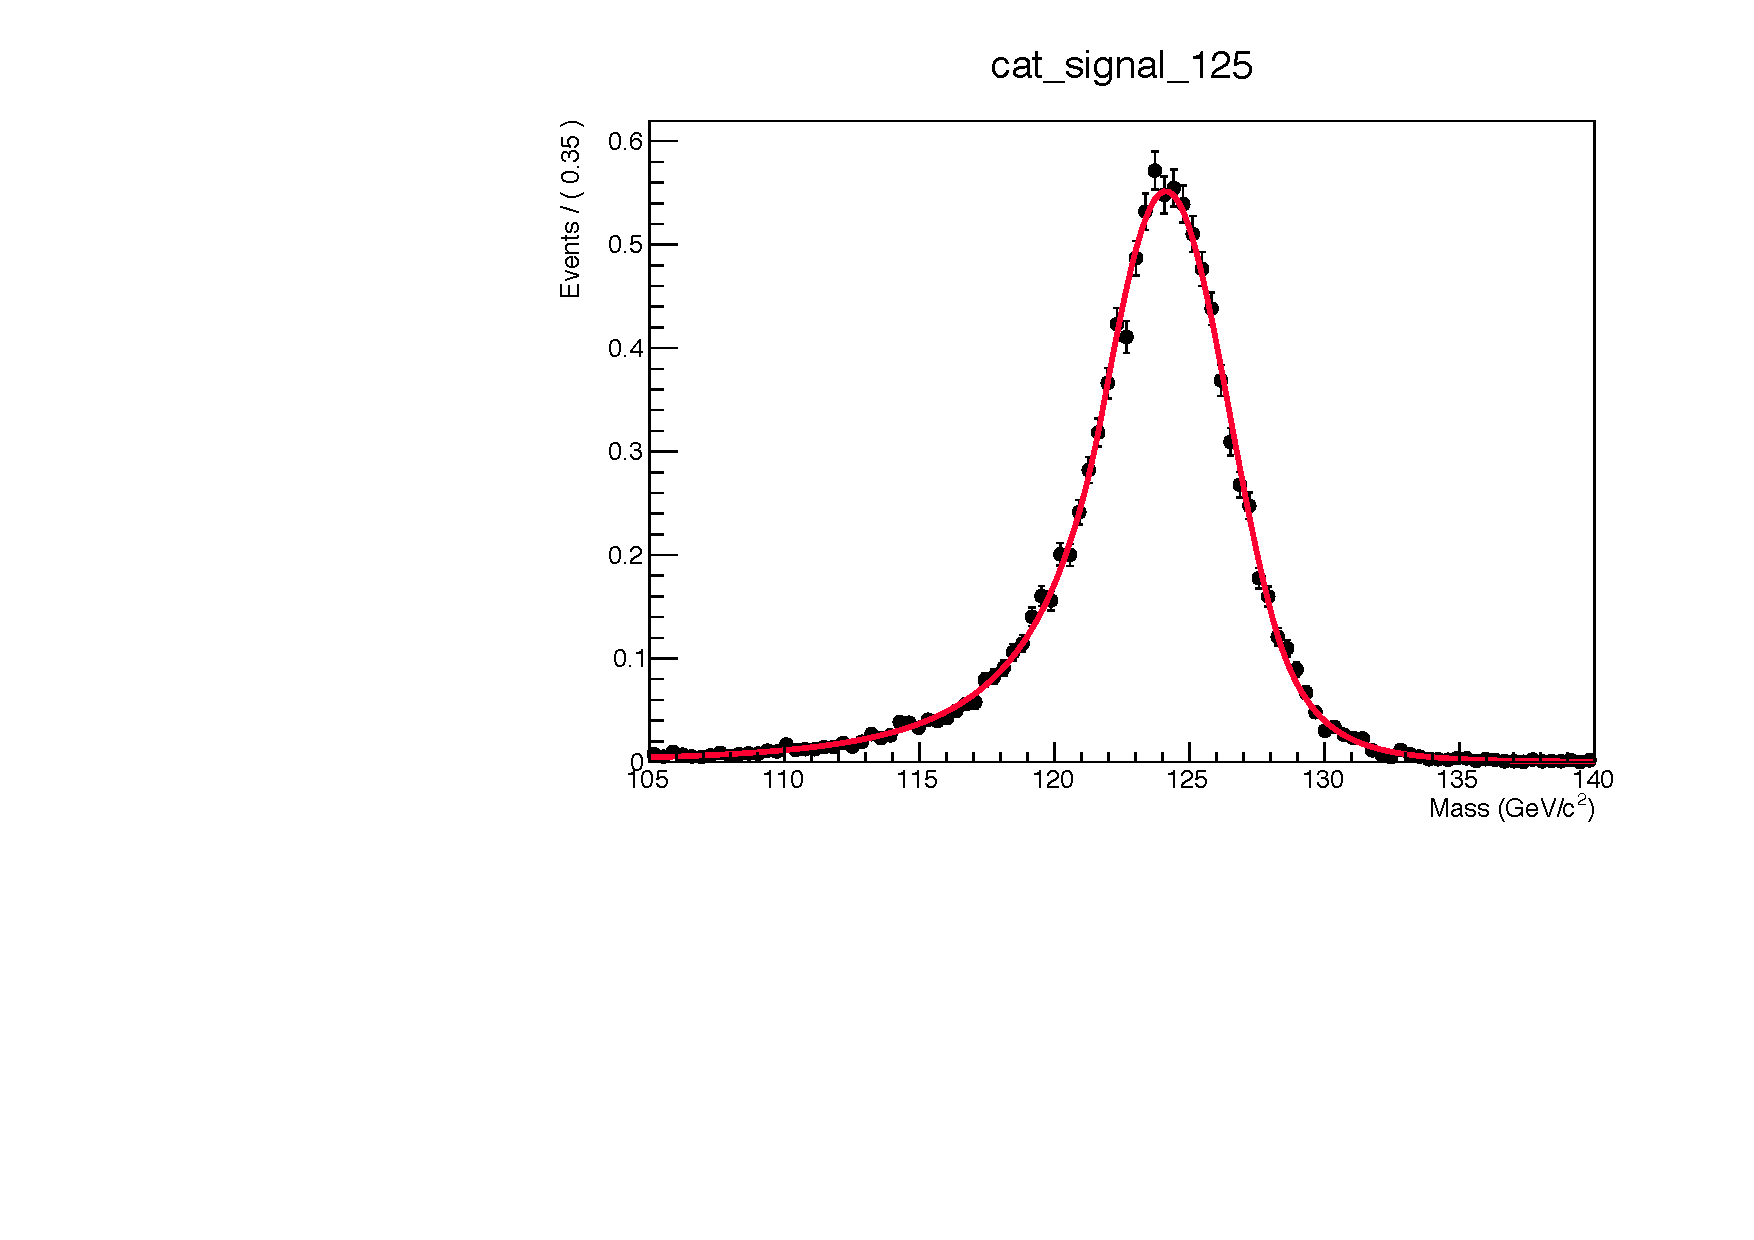
\includegraphics[width=0.3\textwidth]{Figures/SignalModelling/Signal_Parametrization/2017/ggH_4e_2017_125_Sim.pdf}
%		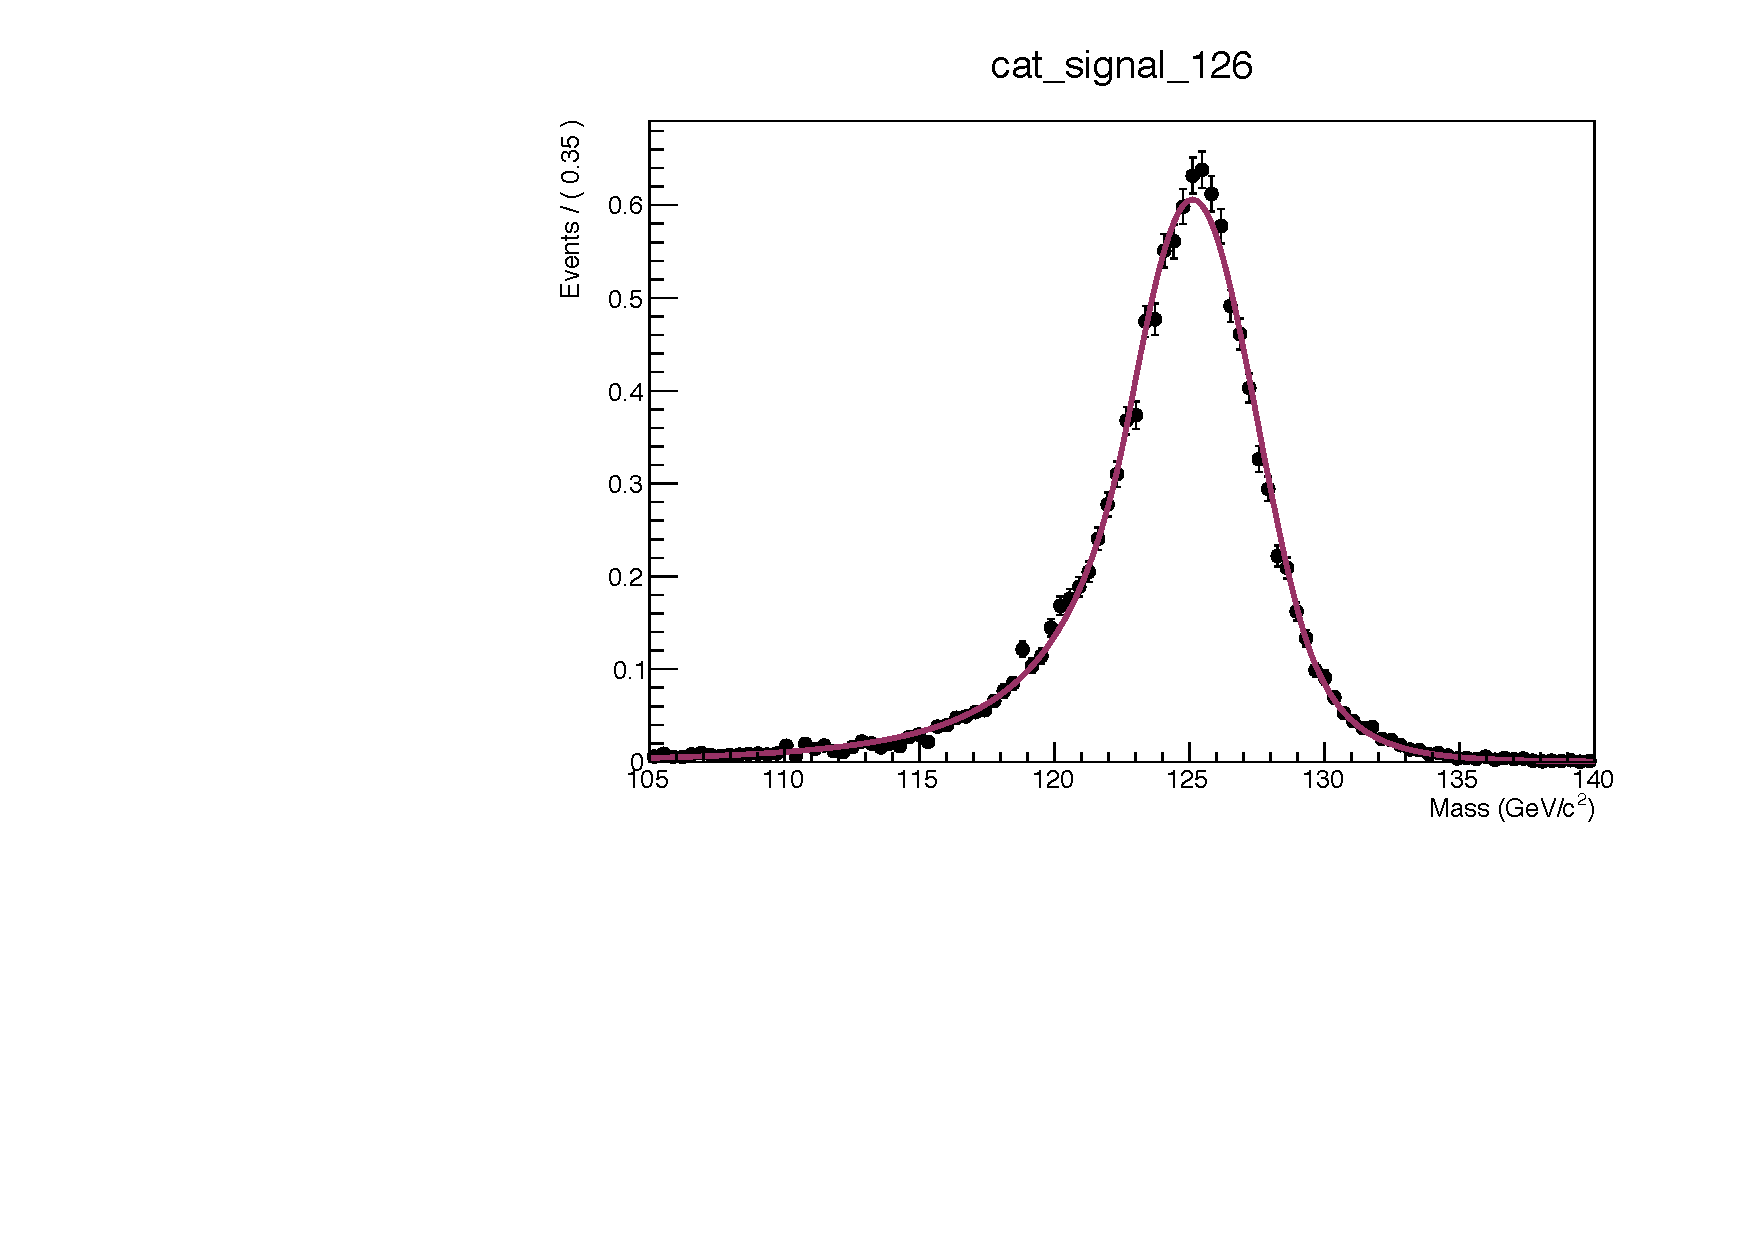
\includegraphics[width=0.3\textwidth]{Figures/SignalModelling/Signal_Parametrization/2017/ggH_4e_2017_126_Sim.pdf} 
%		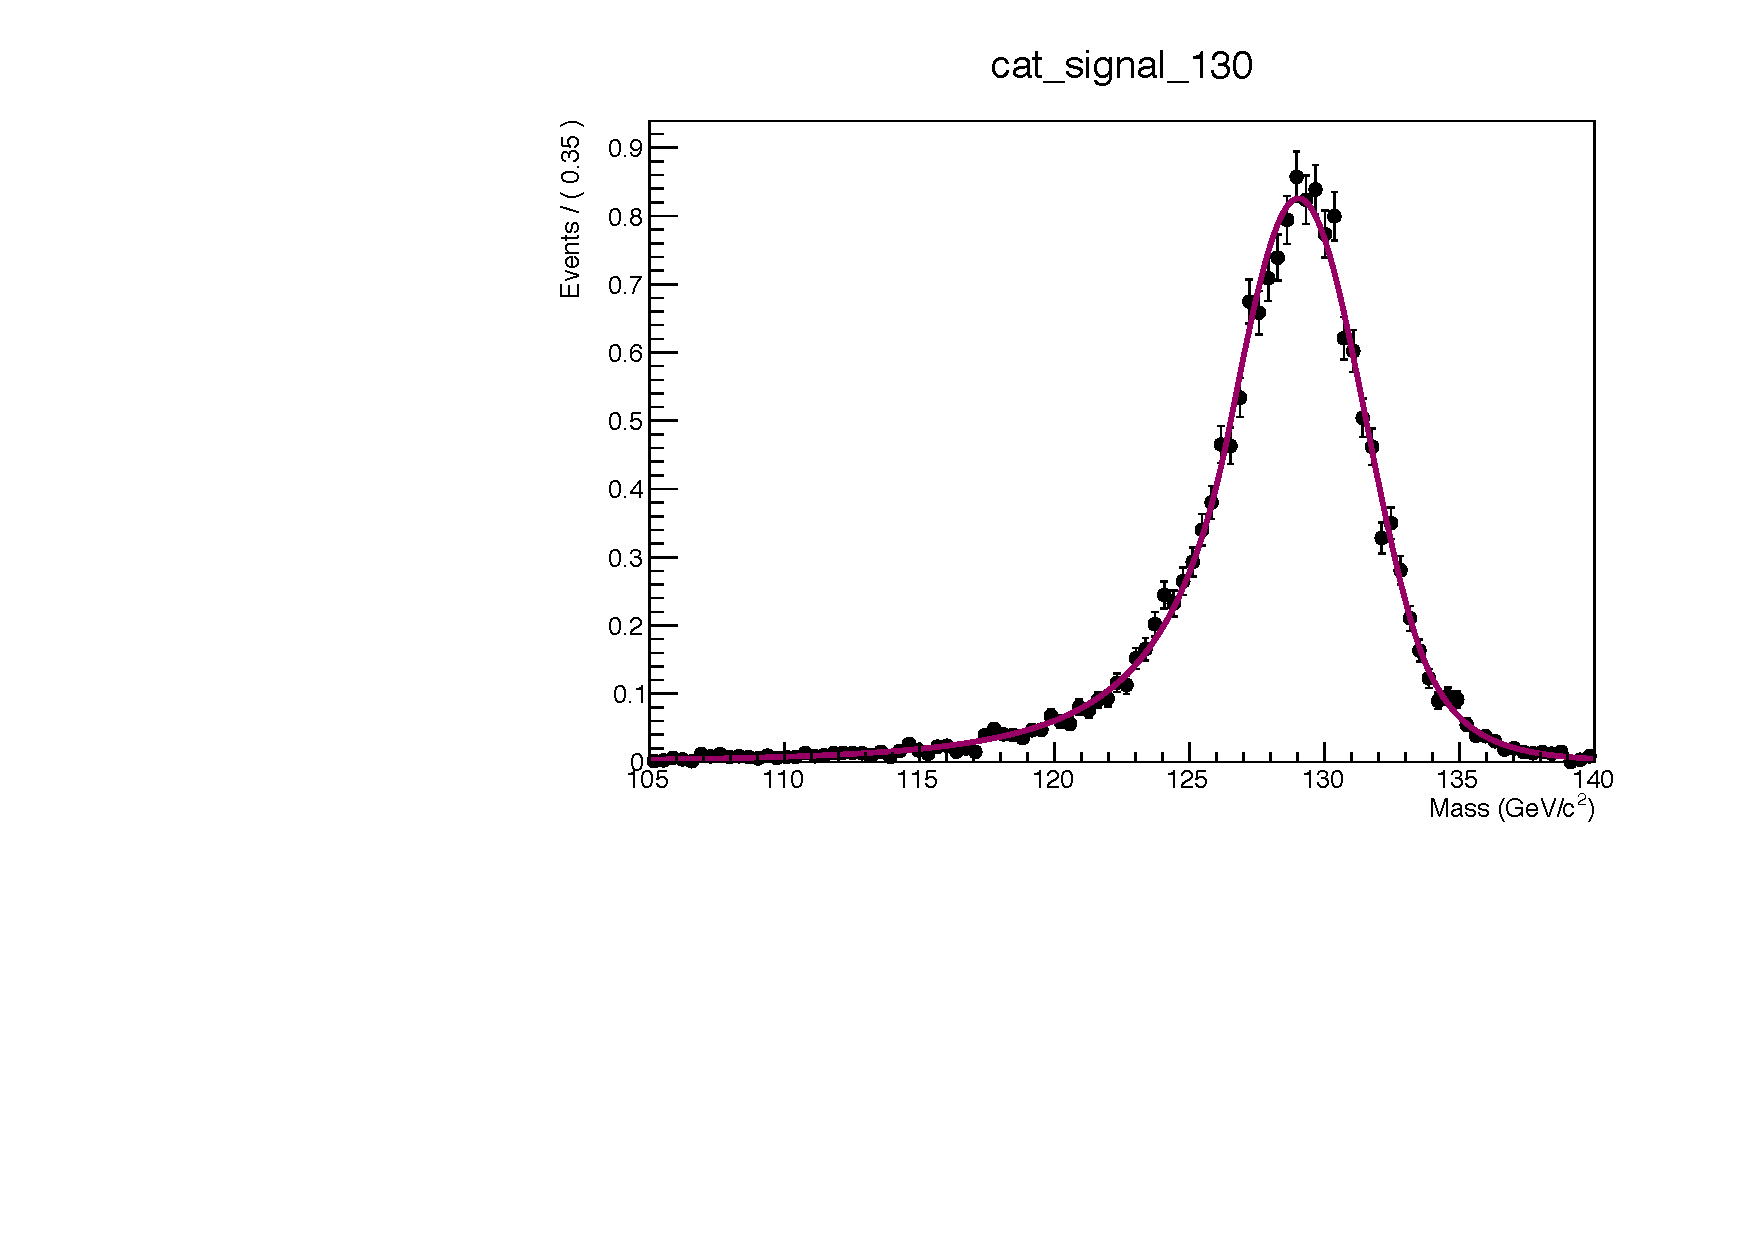
\includegraphics[width=0.3\textwidth]{Figures/SignalModelling/Signal_Parametrization/2017/ggH_4e_2017_130_Sim.pdf}
%		\caption{Simultaneous fit for ggH production mode, in 2017, for different mass points, 
%		in 4e final state.}
%	\label{signal_lineshape_2017_full_1}
%	\end{center}
%\end{figure}
%\begin{figure}[!htbp]
%	\begin{center}
%		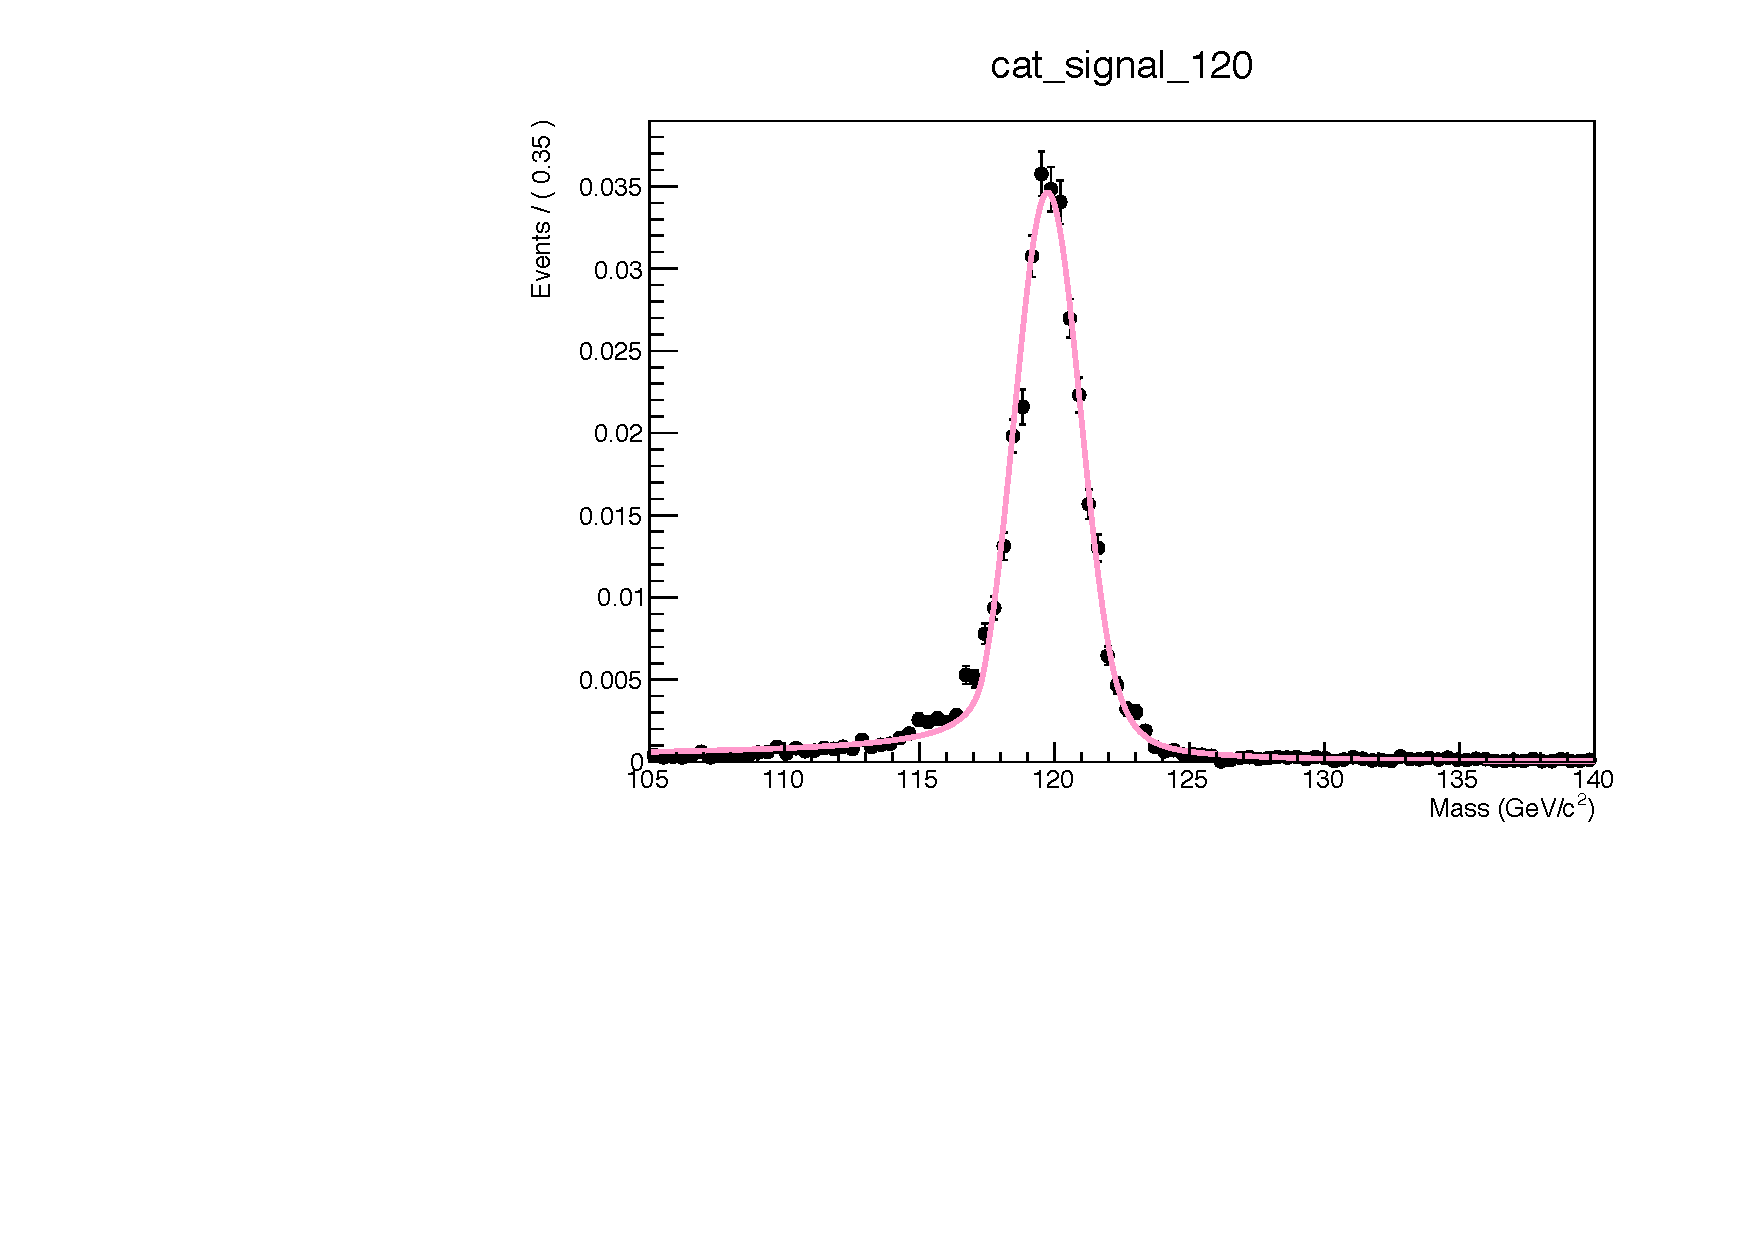
\includegraphics[width=0.3\textwidth]{Figures/SignalModelling/Signal_Parametrization/2017/WH_4mu_2017_120_Sim.pdf}
%		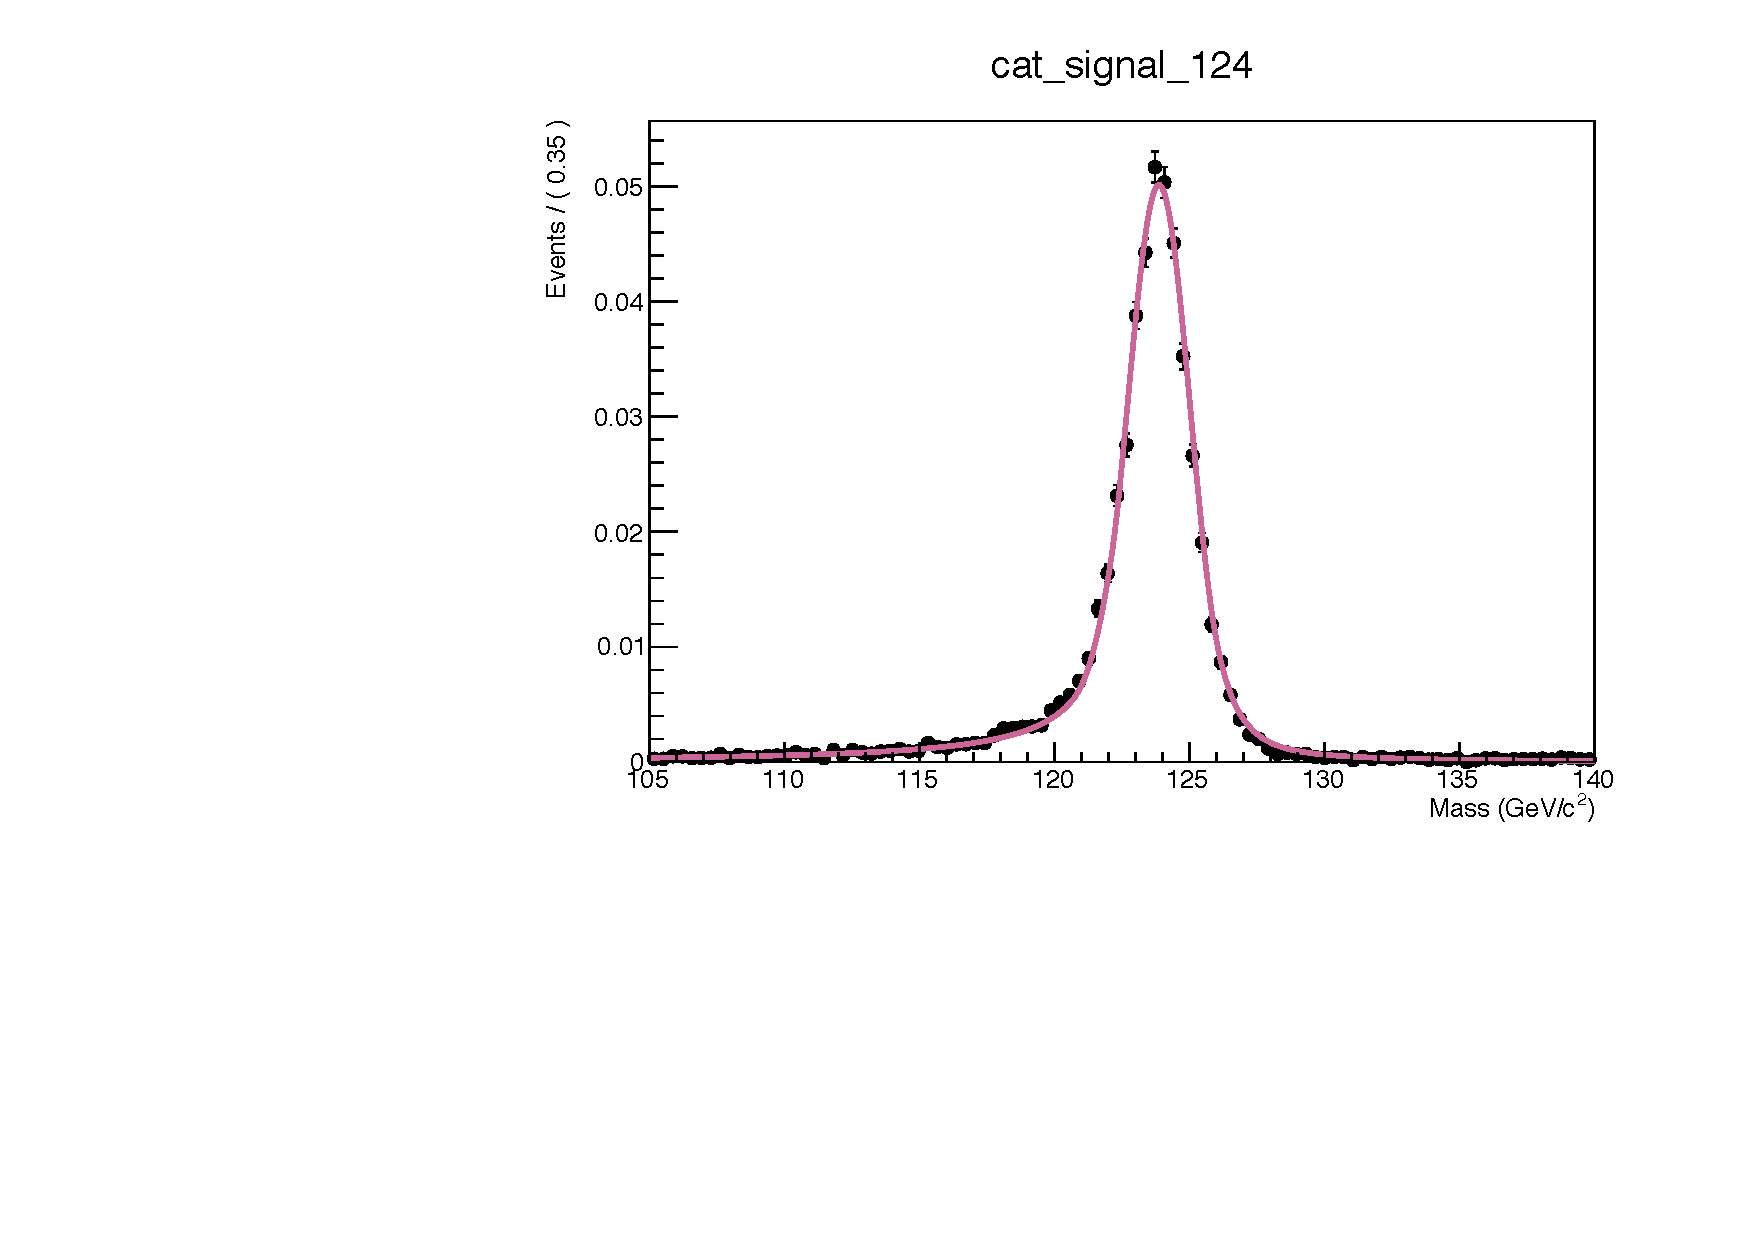
\includegraphics[width=0.3\textwidth]{Figures/SignalModelling/Signal_Parametrization/2017/WH_4mu_2017_124_Sim.pdf}
%   		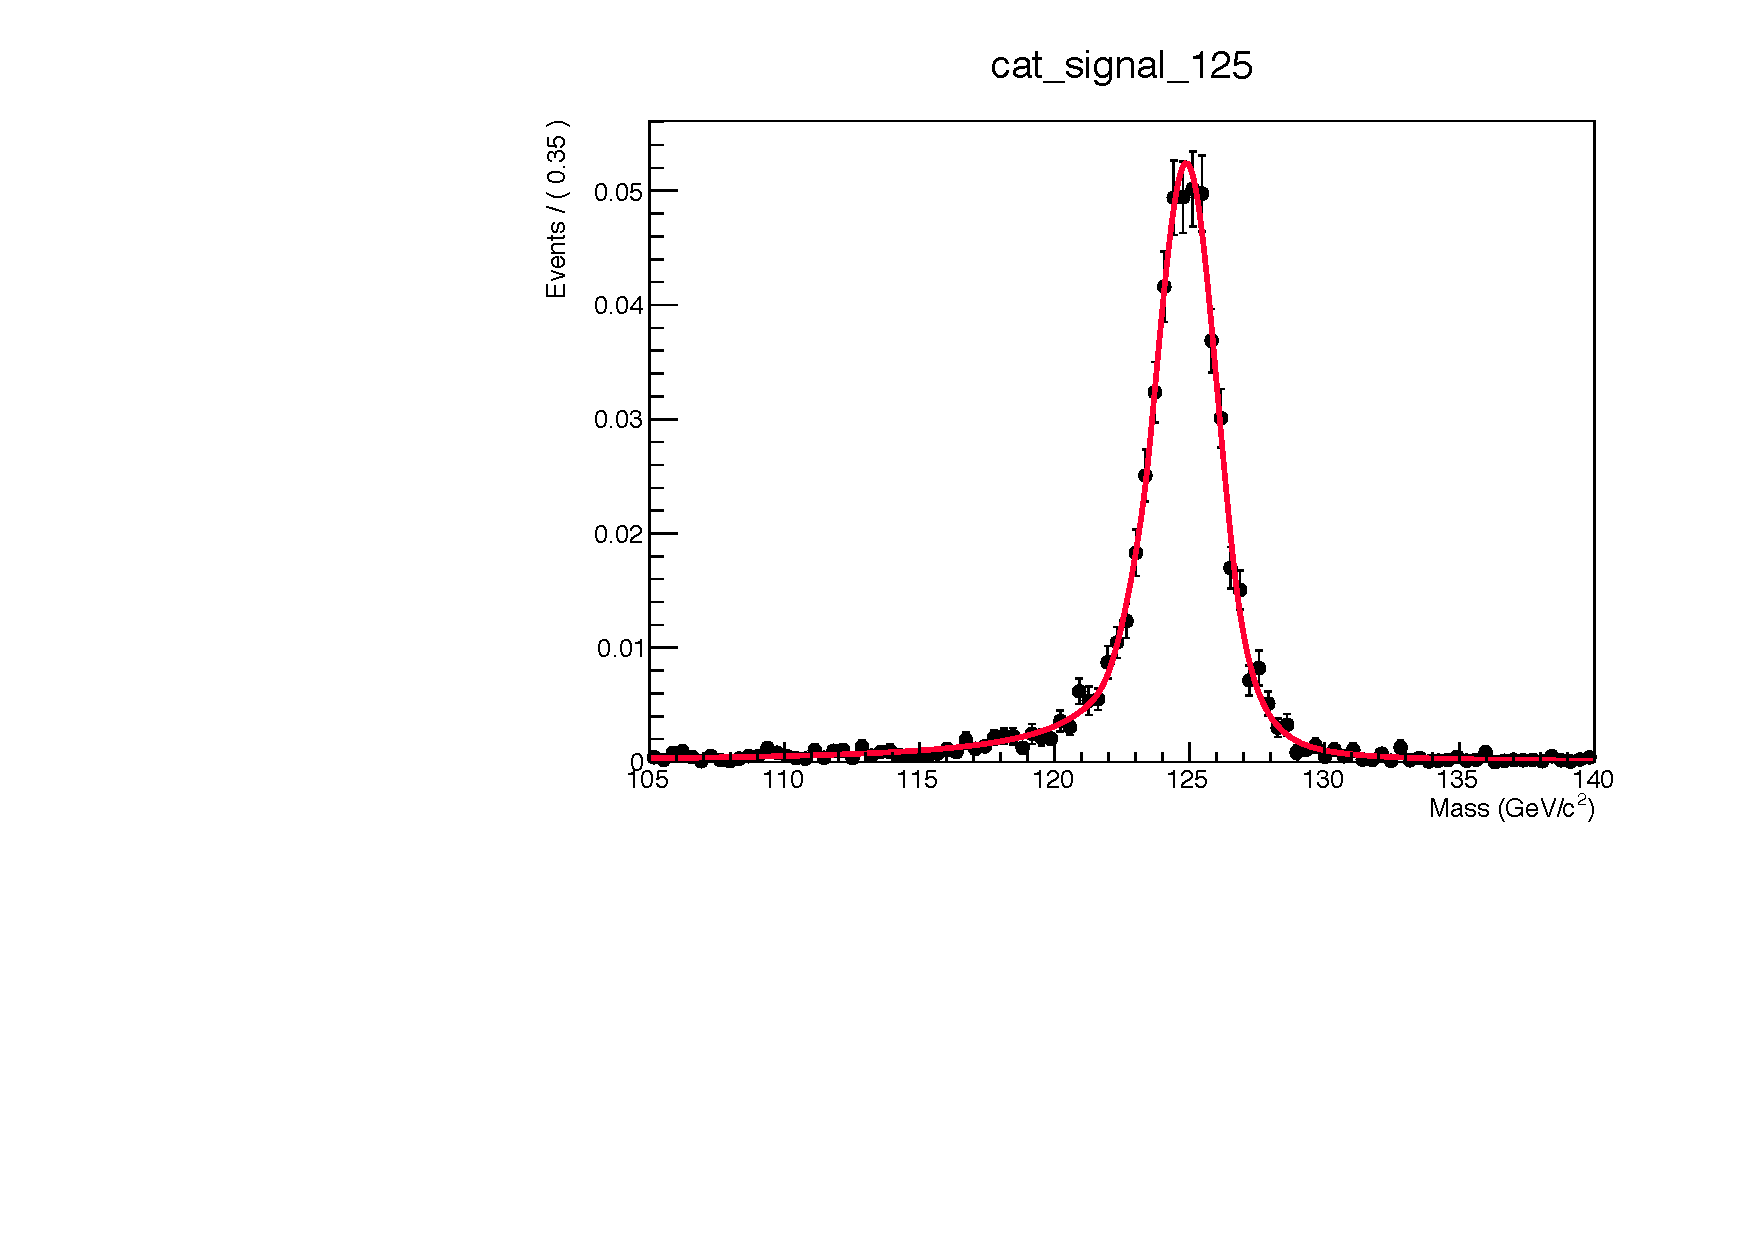
\includegraphics[width=0.3\textwidth]{Figures/SignalModelling/Signal_Parametrization/2017/WH_4mu_2017_125_Sim.pdf}
%		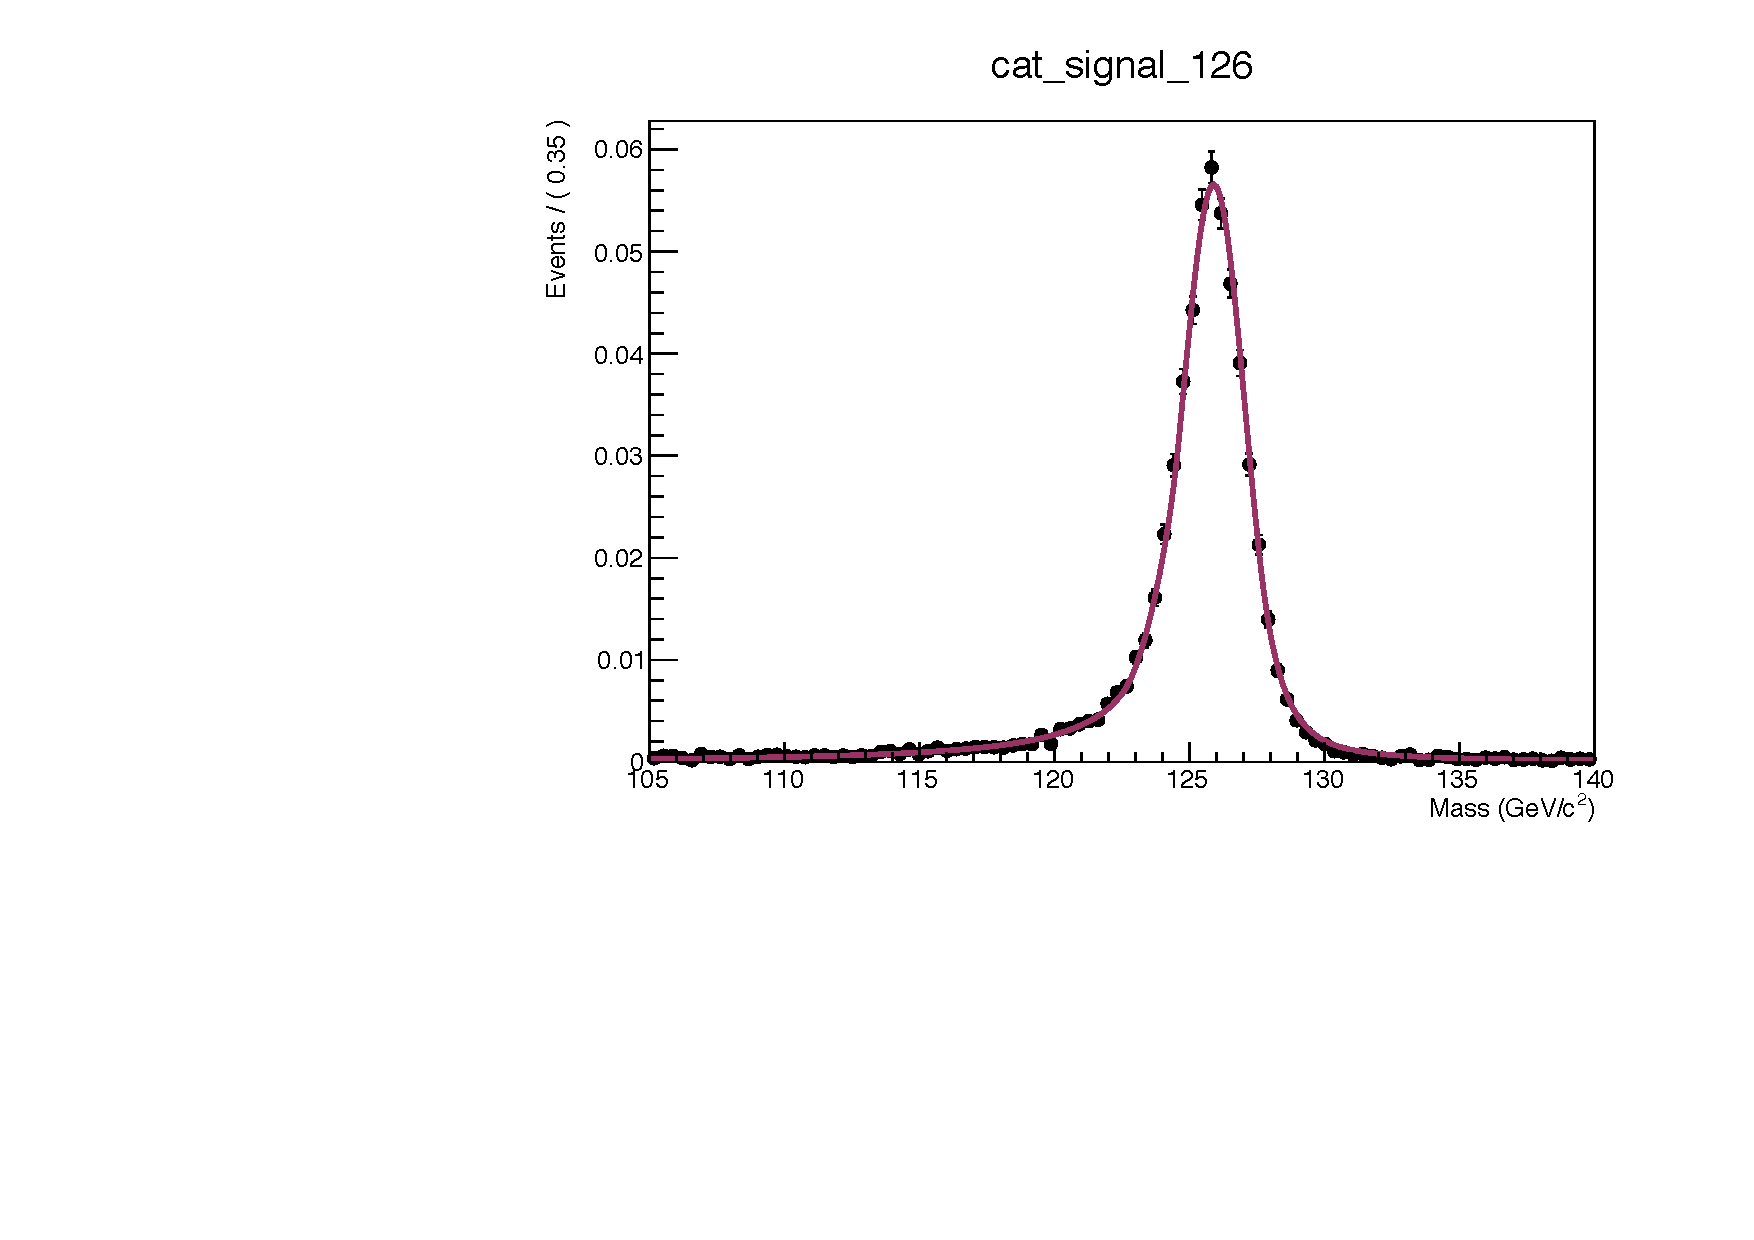
\includegraphics[width=0.3\textwidth]{Figures/SignalModelling/Signal_Parametrization/2017/WH_4mu_2017_126_Sim.pdf} 
%		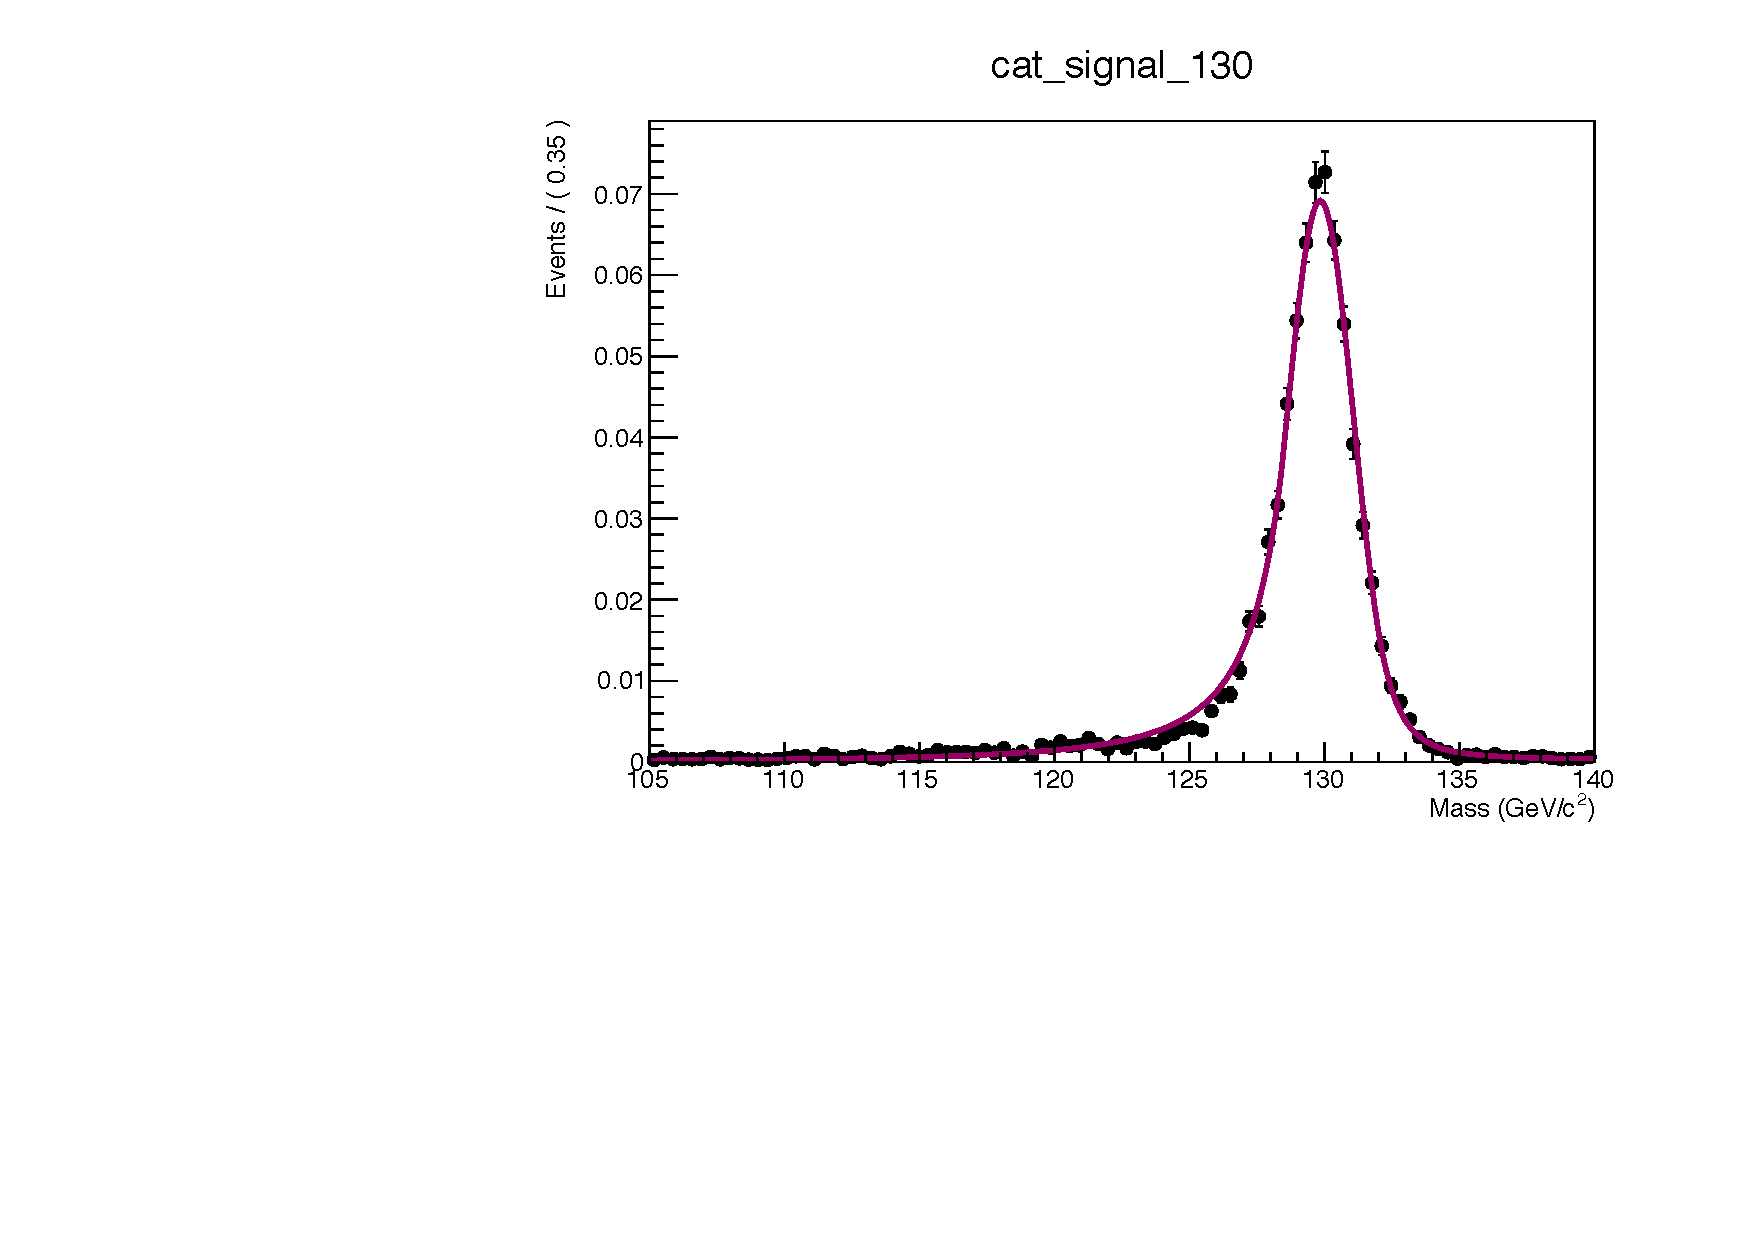
\includegraphics[width=0.3\textwidth]{Figures/SignalModelling/Signal_Parametrization/2017/WH_4mu_2017_130_Sim.pdf}
%		\caption{Simultaneous fit for WH production mode, in 2017, for different mass points, 
%		in 4$\mu$ final state.}
%	\label{signal_lineshape_2017_full_2}
%	\end{center}
%\end{figure}
%\begin{figure}[!htbp]
%	\begin{center}
%		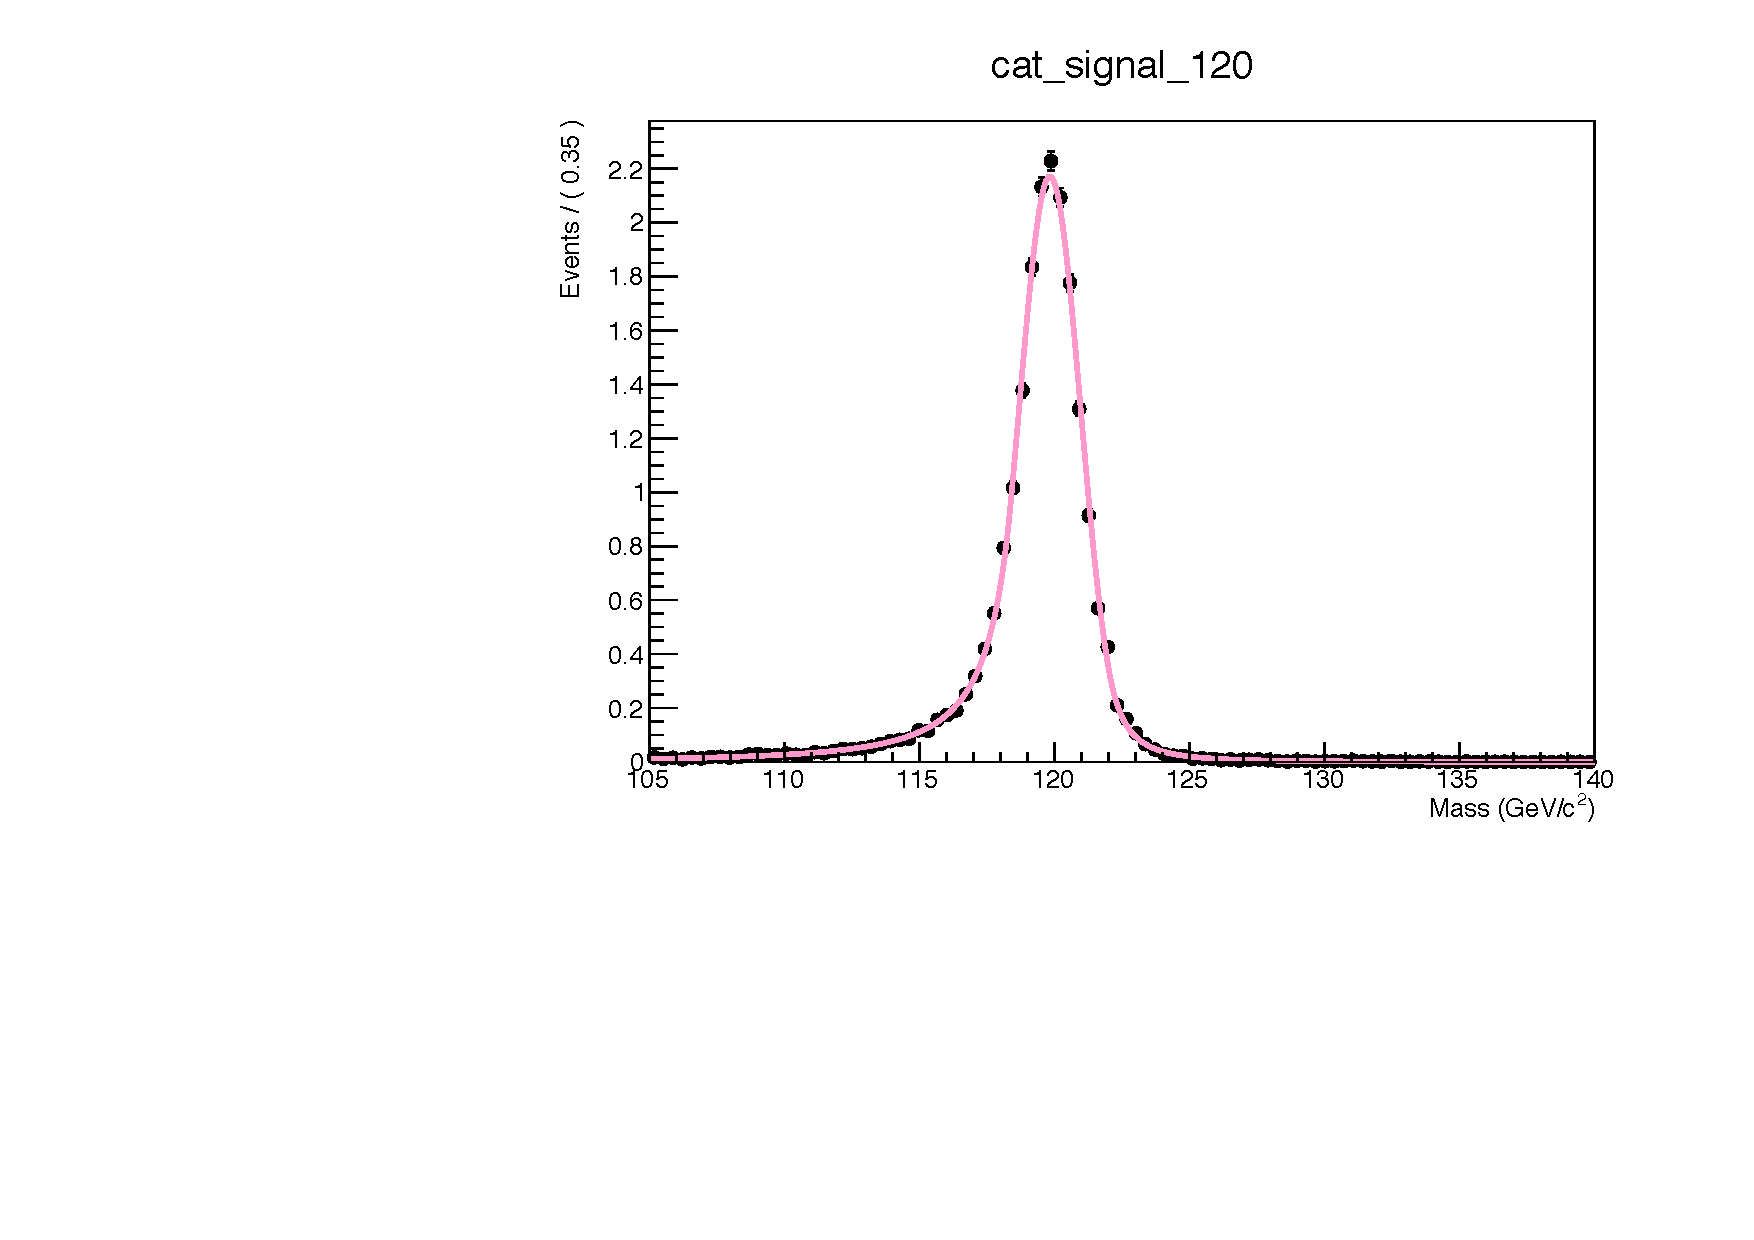
\includegraphics[width=0.3\textwidth]{Figures/SignalModelling/Signal_Parametrization/2018/ggH_4mu_2018_120_Sim.pdf}
%		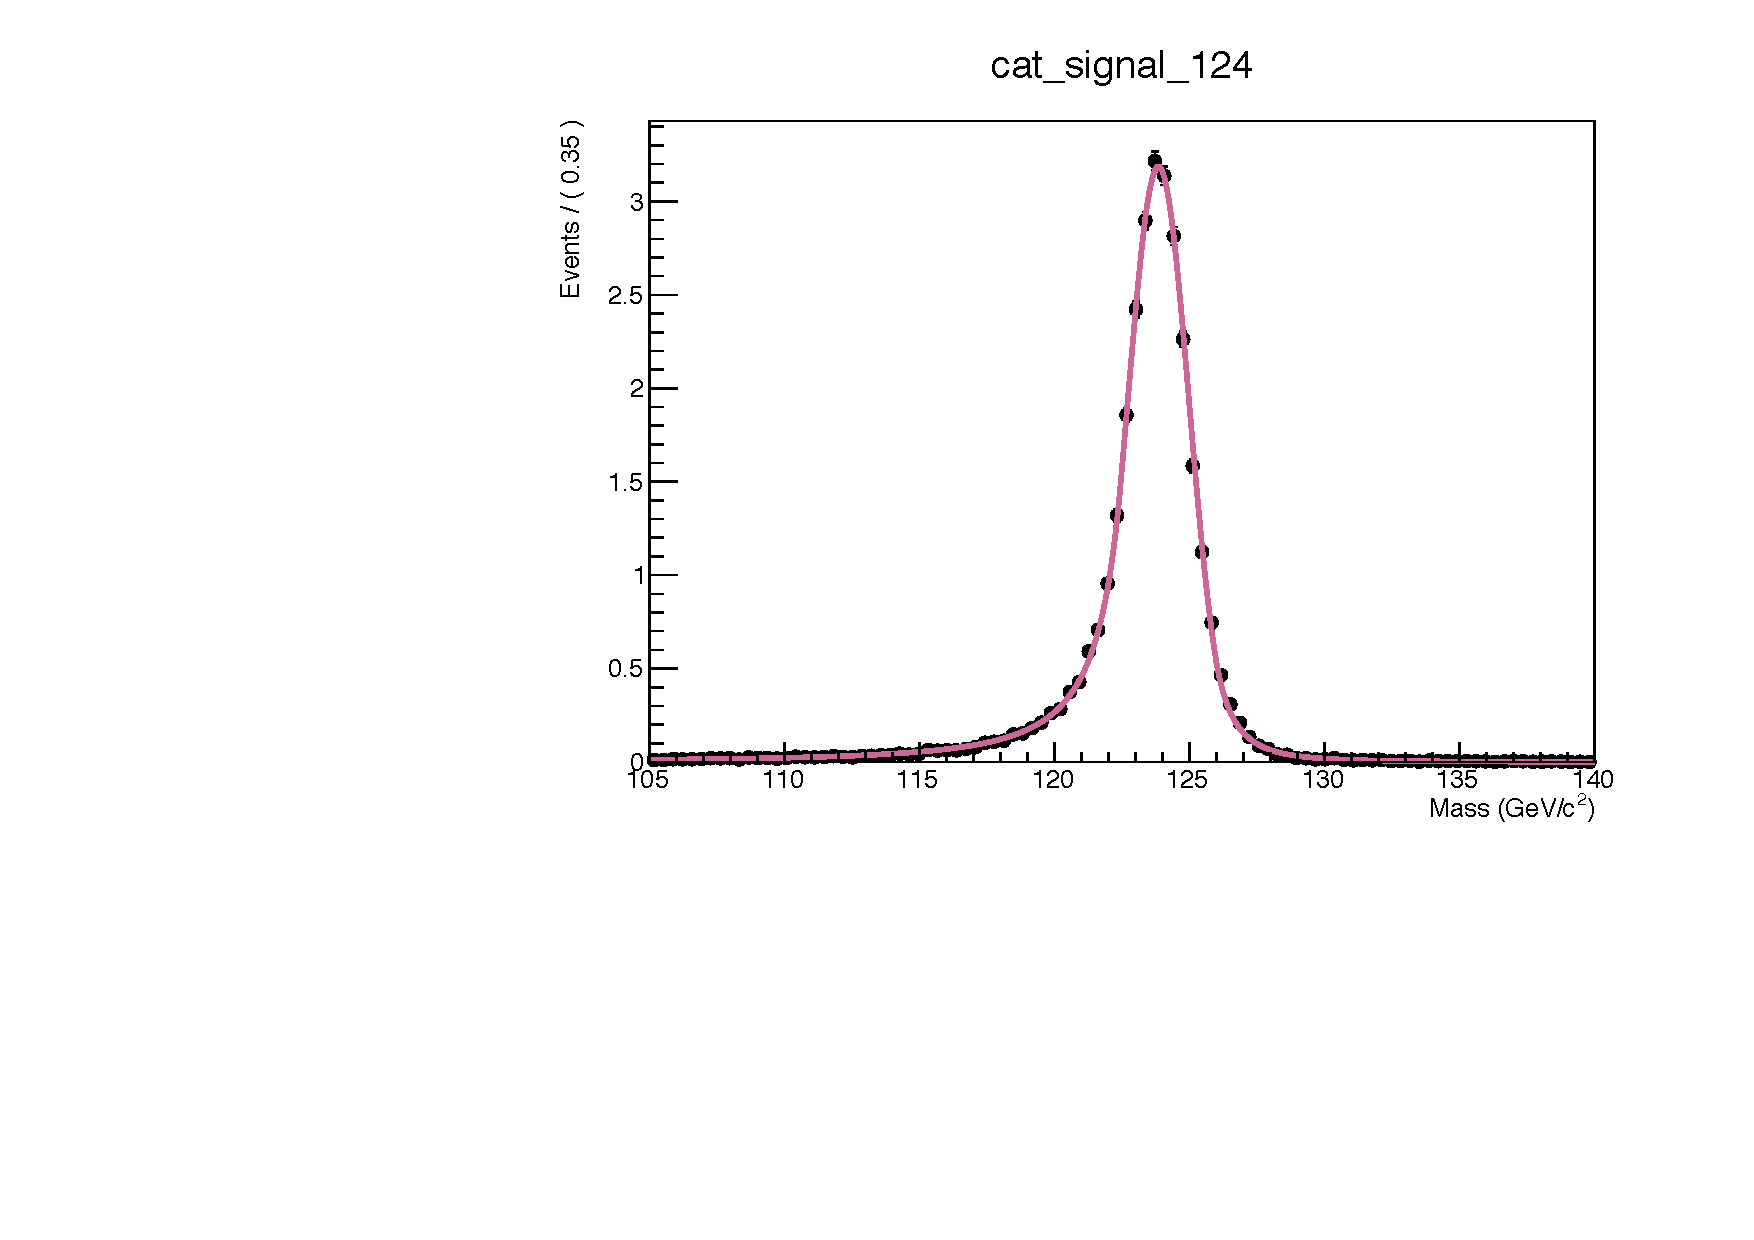
\includegraphics[width=0.3\textwidth]{Figures/SignalModelling/Signal_Parametrization/2018/ggH_4mu_2018_124_Sim.pdf}
%   		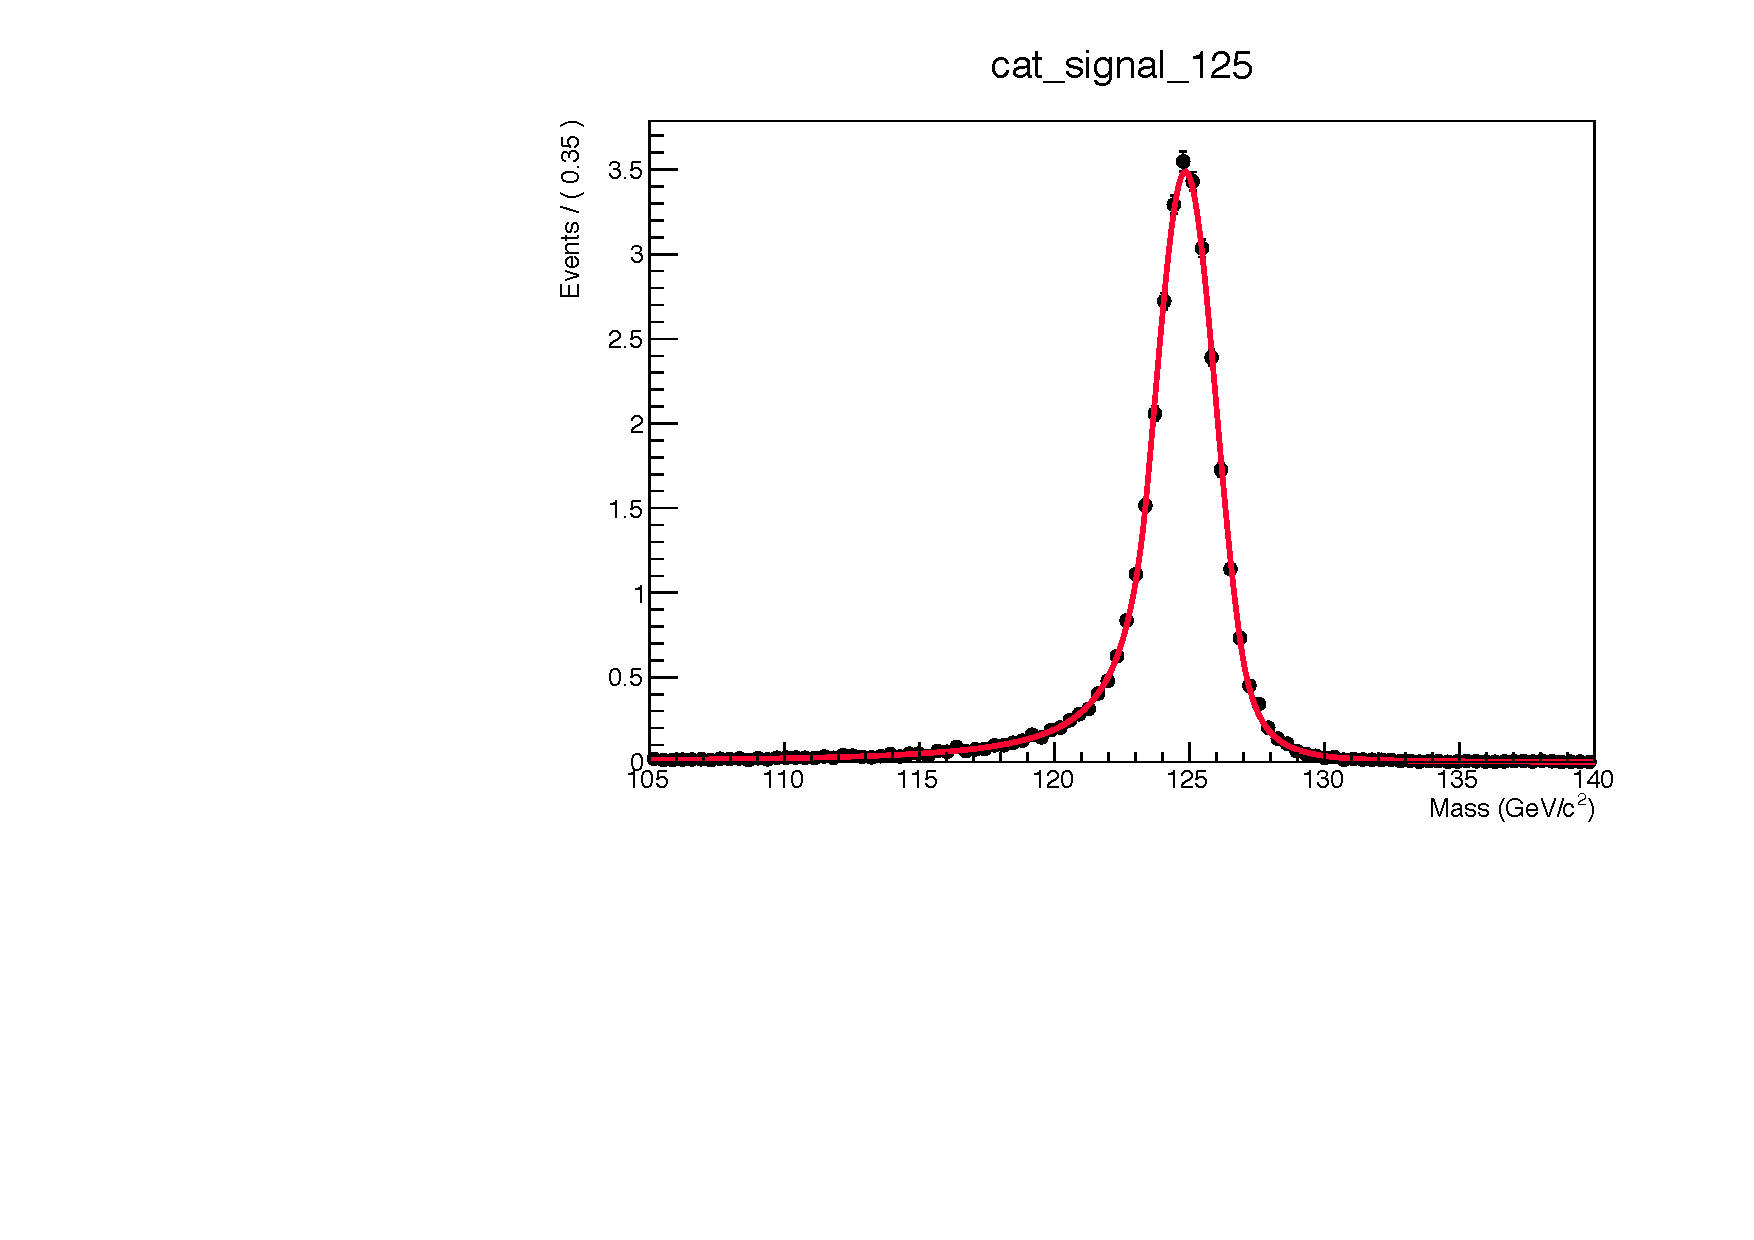
\includegraphics[width=0.3\textwidth]{Figures/SignalModelling/Signal_Parametrization/2018/ggH_4mu_2018_125_Sim.pdf}
%		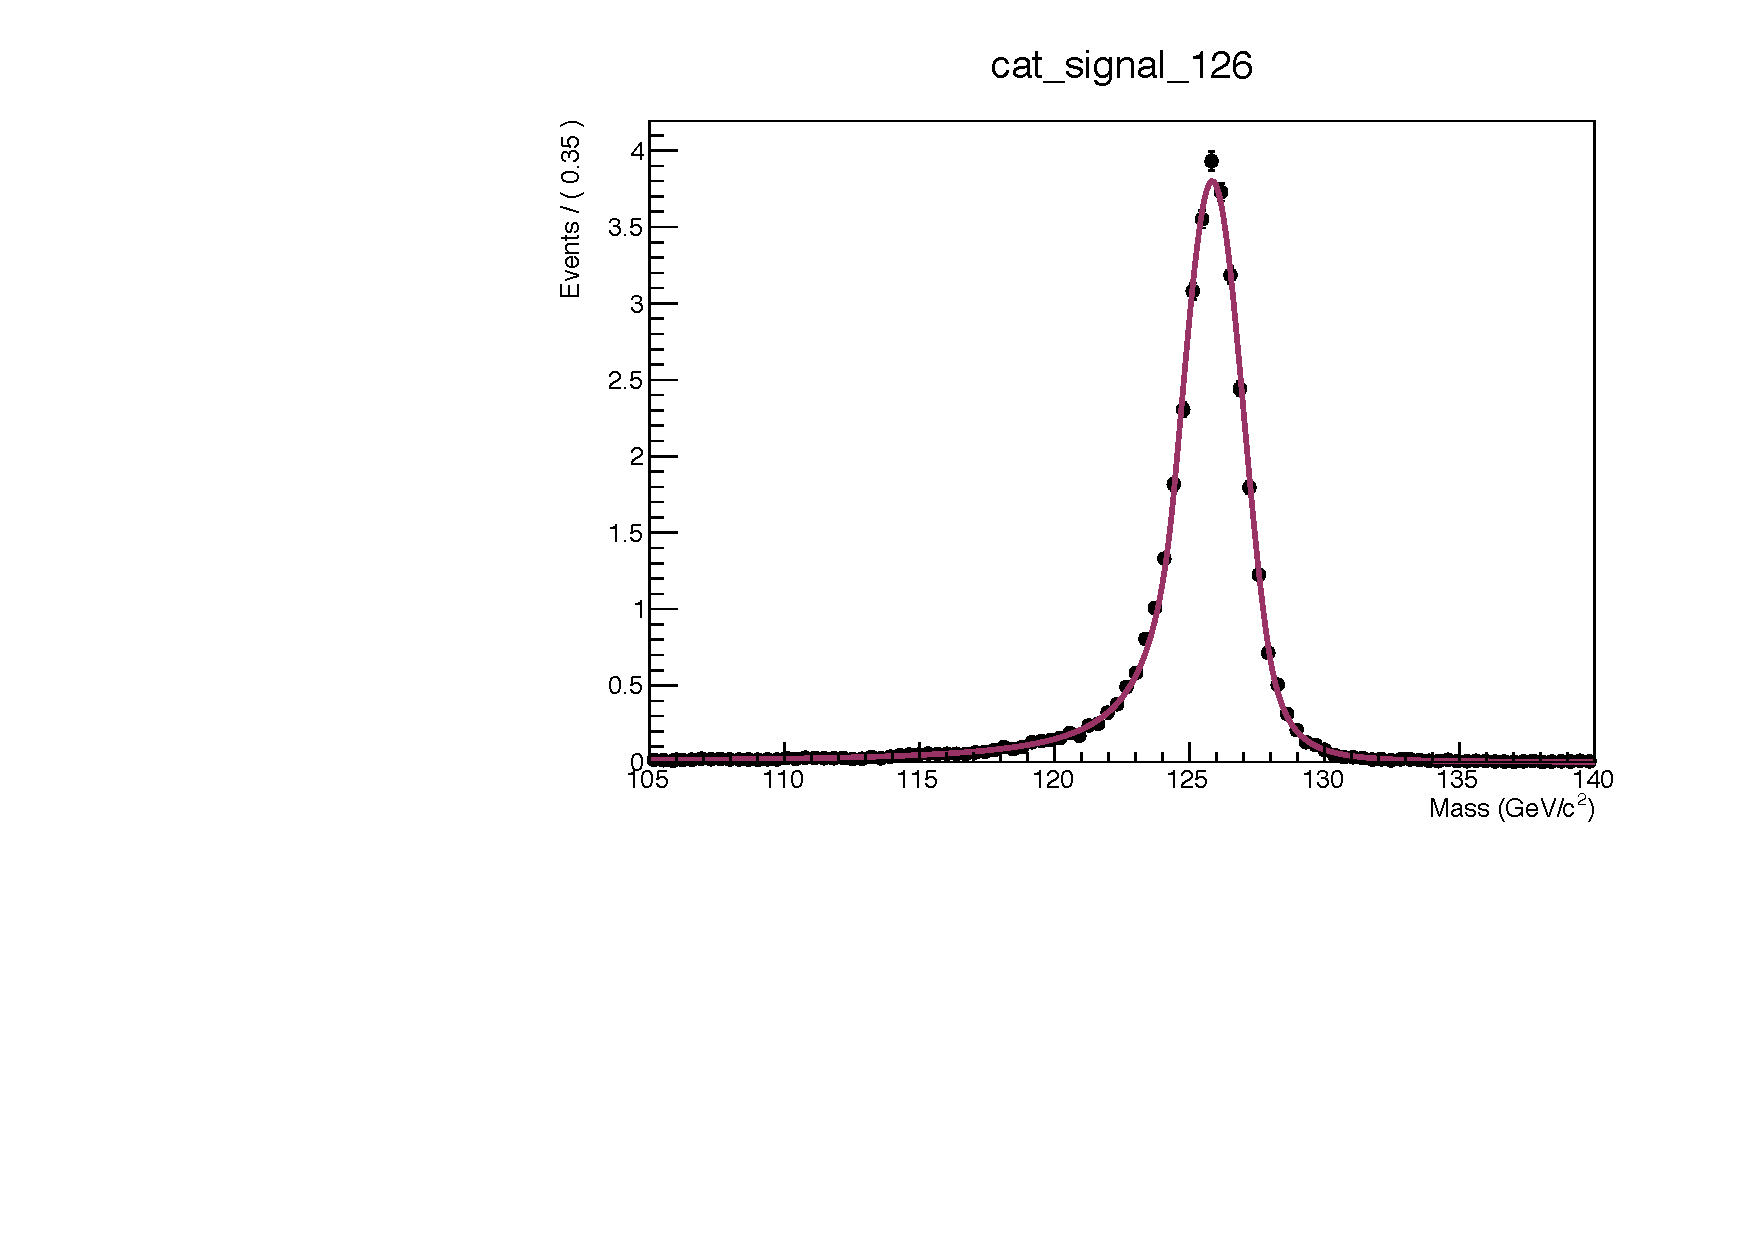
\includegraphics[width=0.3\textwidth]{Figures/SignalModelling/Signal_Parametrization/2018/ggH_4mu_2018_126_Sim.pdf} 
%		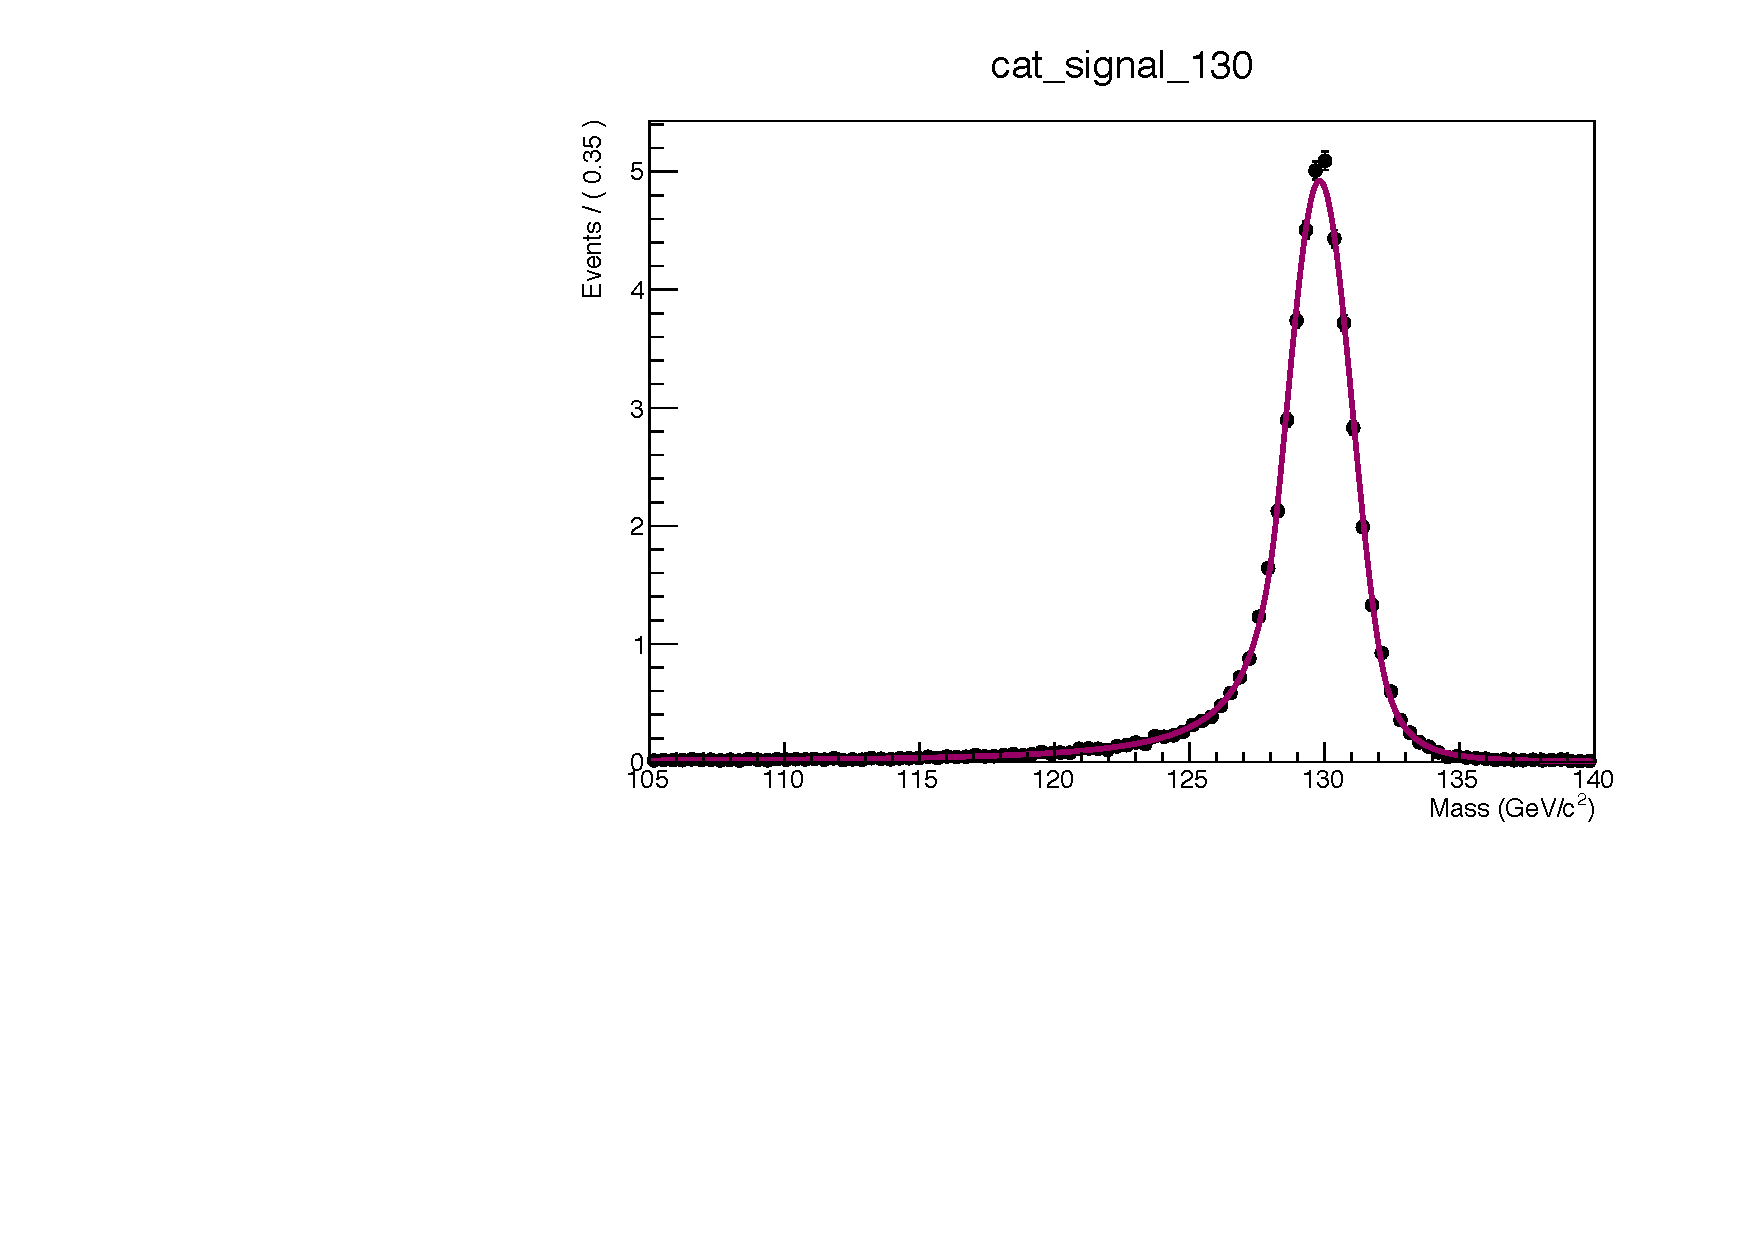
\includegraphics[width=0.3\textwidth]{Figures/SignalModelling/Signal_Parametrization/2018/ggH_4mu_2018_130_Sim.pdf}
%		\caption{Simultaneous fit for ggH production mode, in 2018, for different mass points, 
%		in 4$\mu$ final state.}
%	\label{signal_lineshape_2018_full_1}
%	\end{center}
%\end{figure}
%\begin{figure}[!htbp]
%	\begin{center}
%		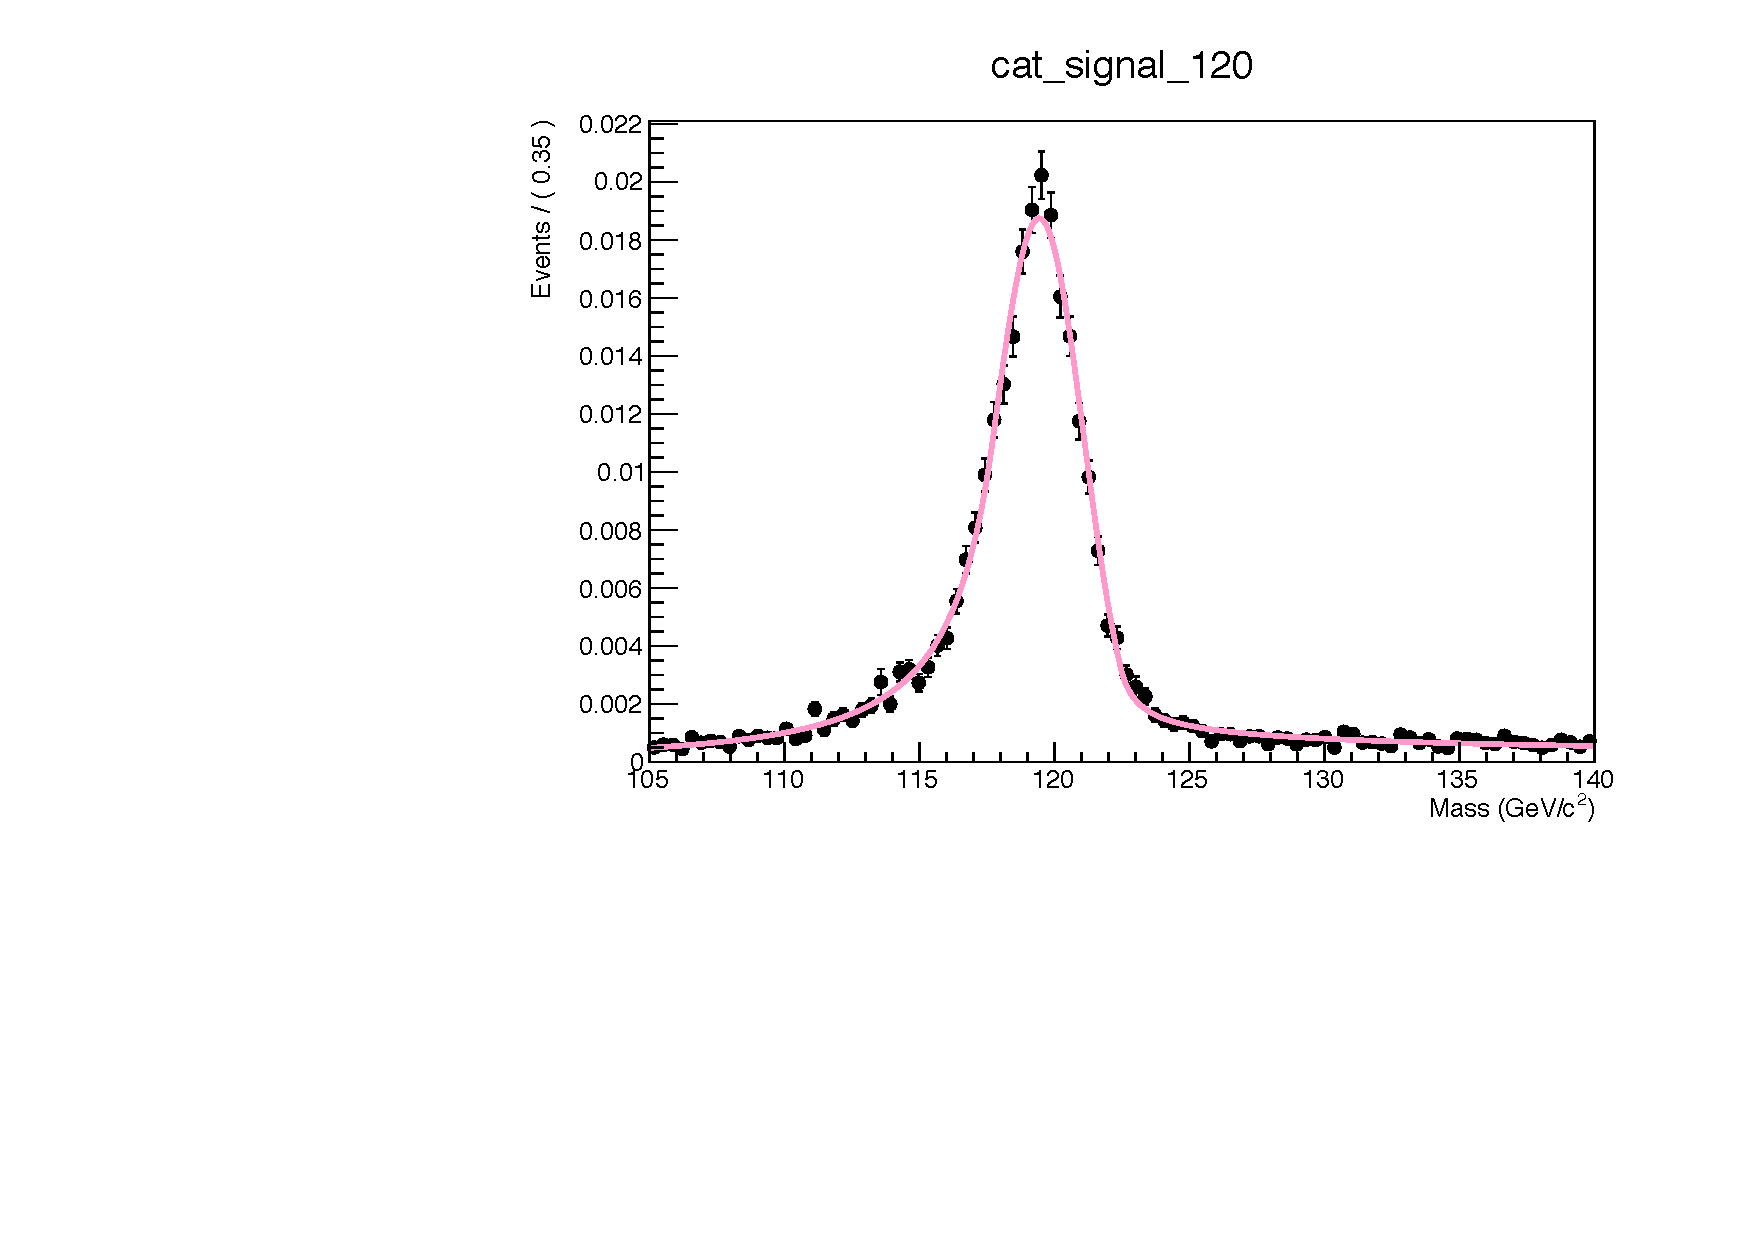
\includegraphics[width=0.3\textwidth]{Figures/SignalModelling/Signal_Parametrization/2018/ttH_2e2mu_2018_120_Sim.pdf}
%		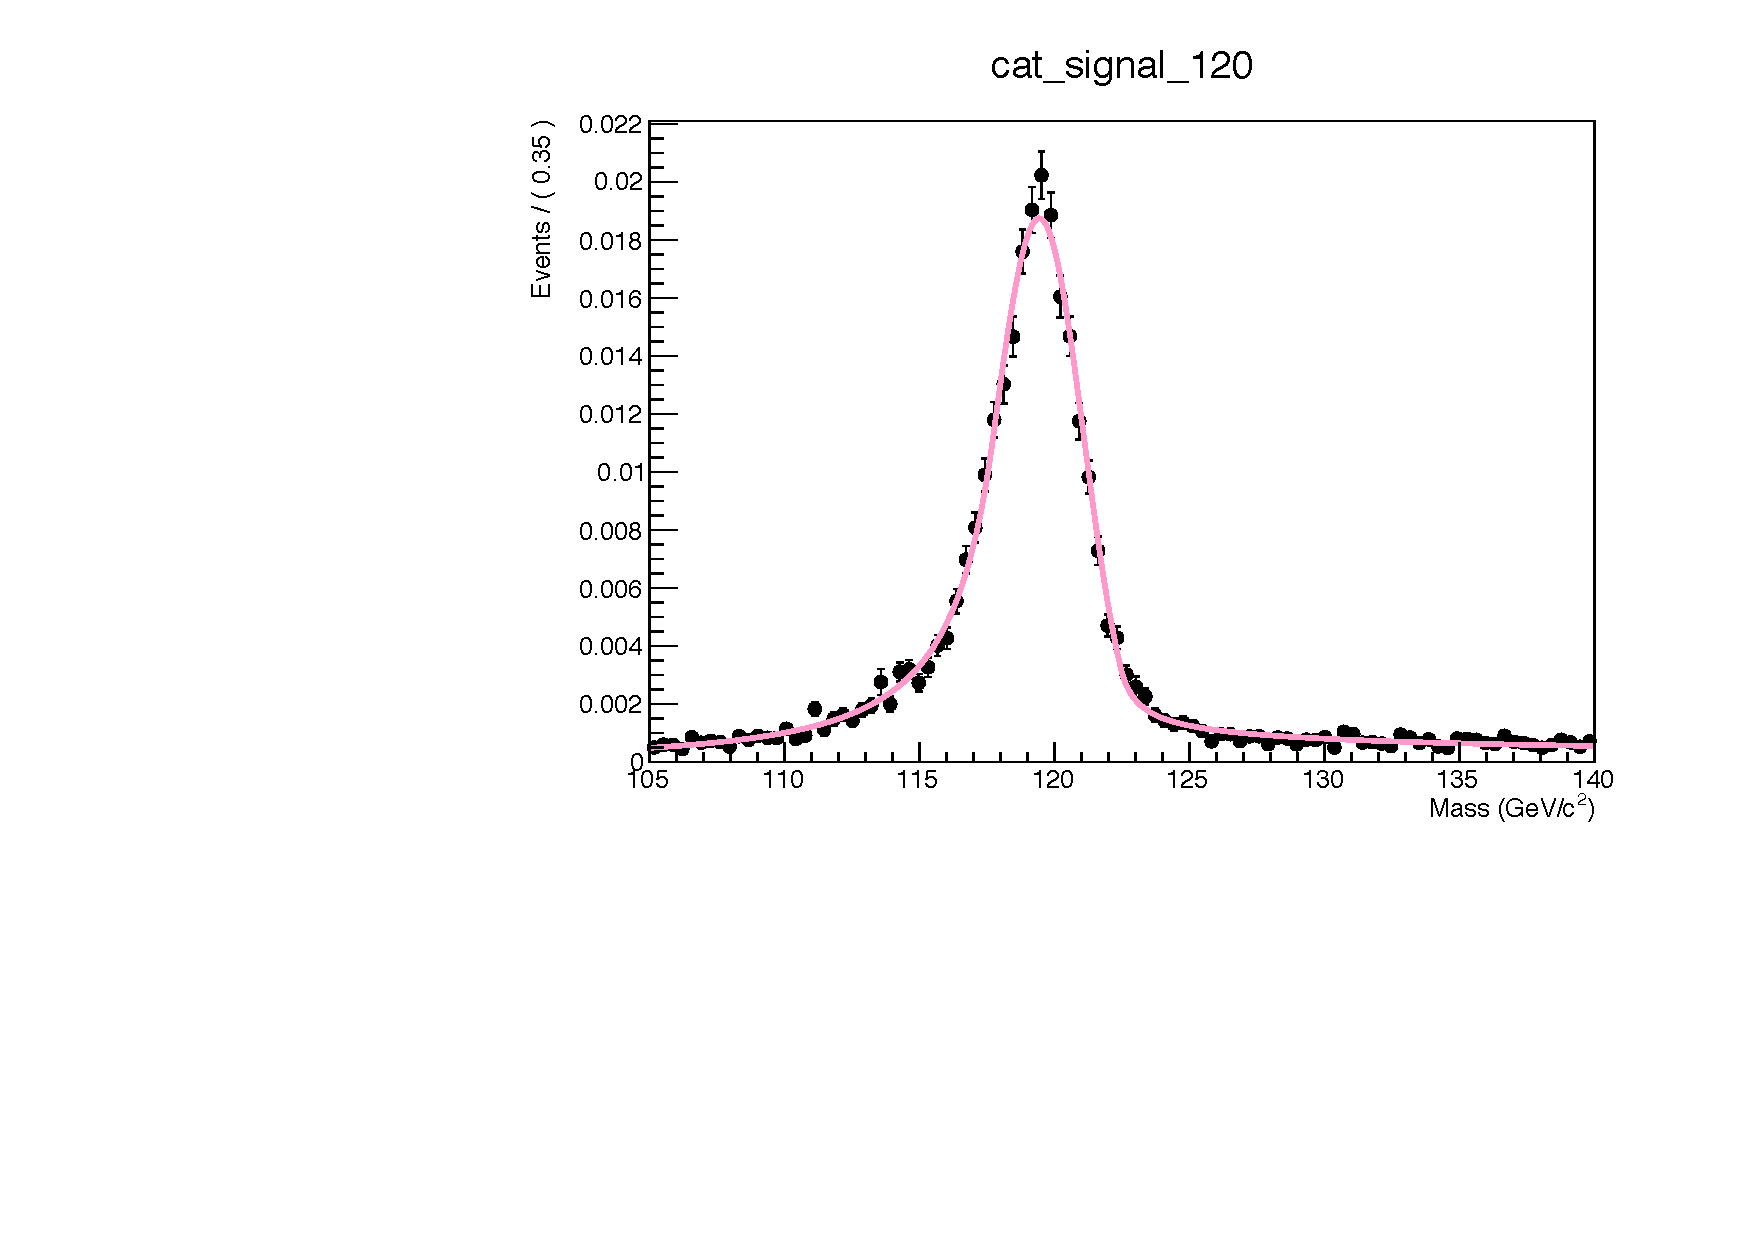
\includegraphics[width=0.3\textwidth]{Figures/SignalModelling/Signal_Parametrization/2018/ttH_2e2mu_2018_120_Sim.pdf}
%   		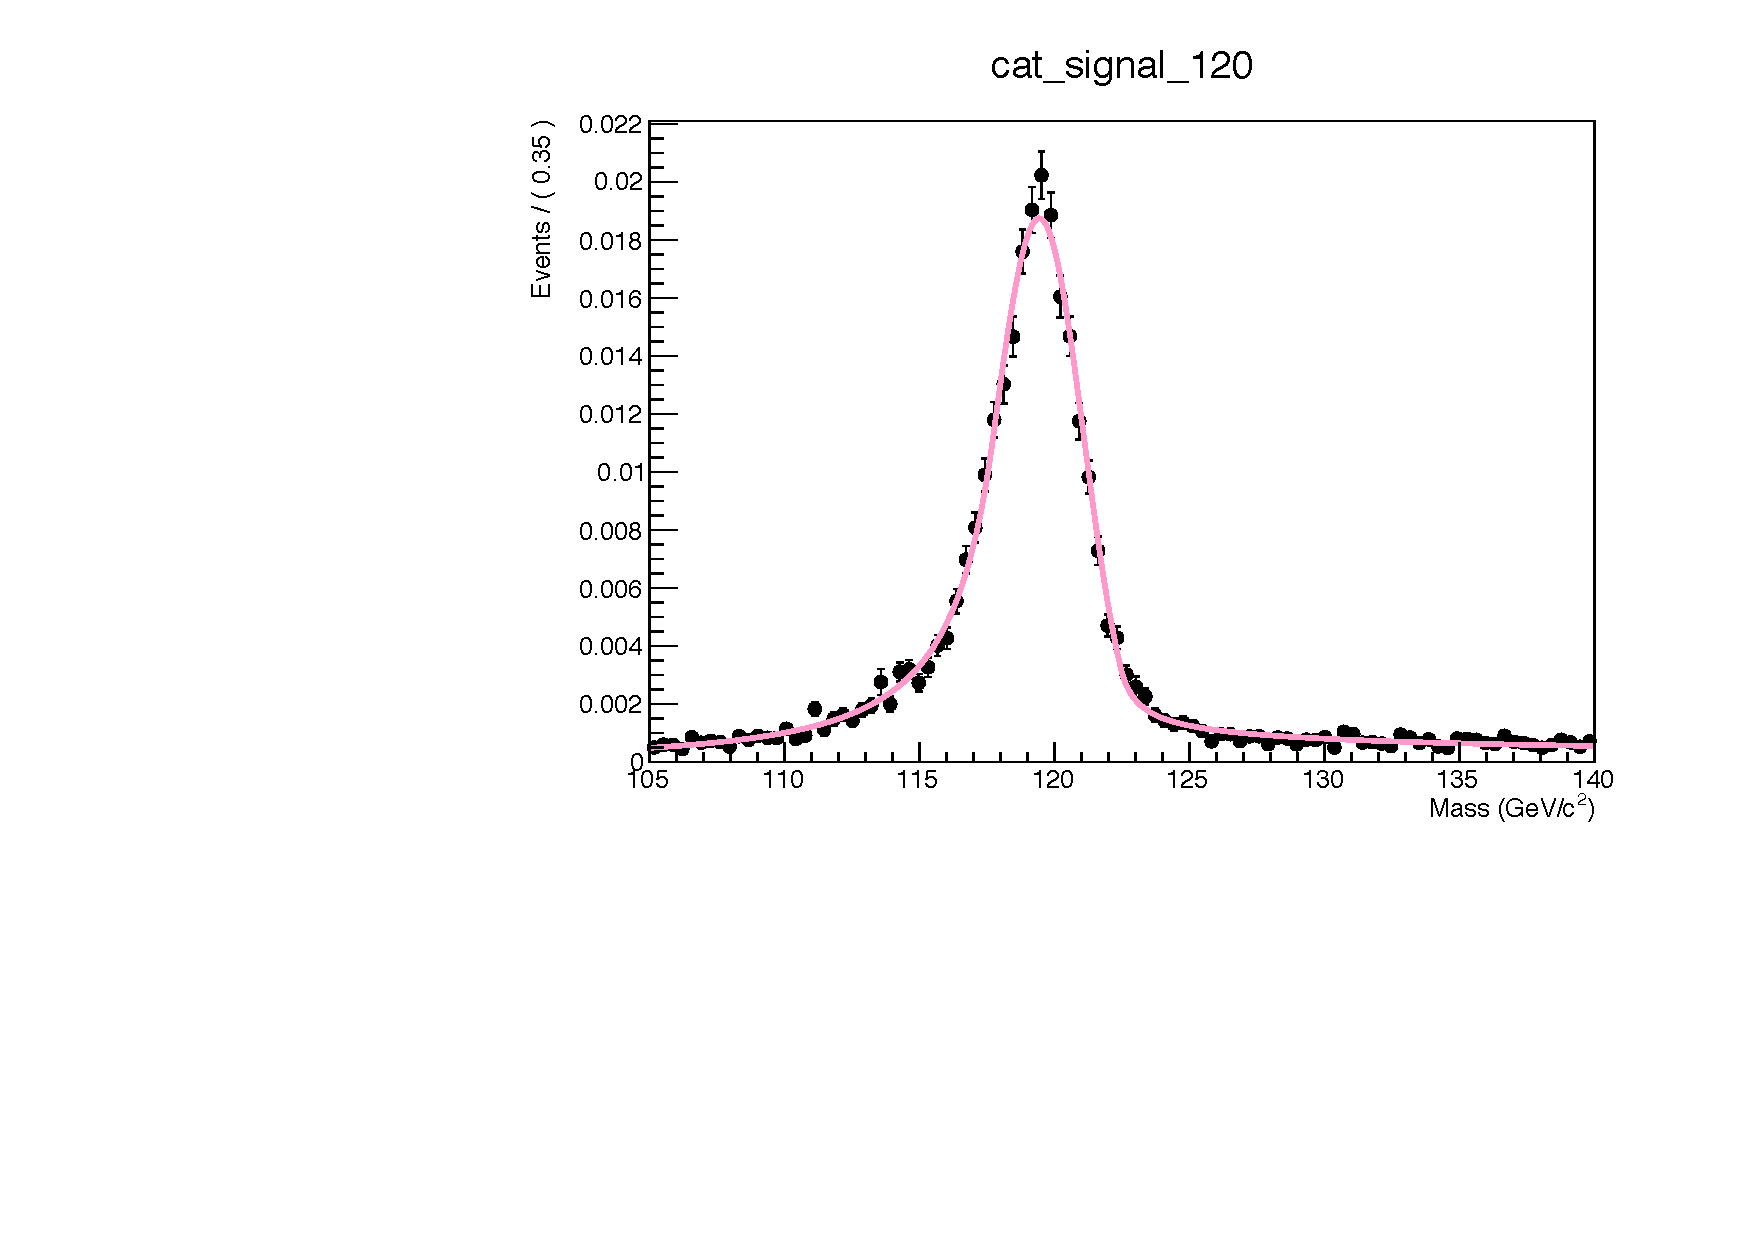
\includegraphics[width=0.3\textwidth]{Figures/SignalModelling/Signal_Parametrization/2018/ttH_2e2mu_2018_120_Sim.pdf}
%		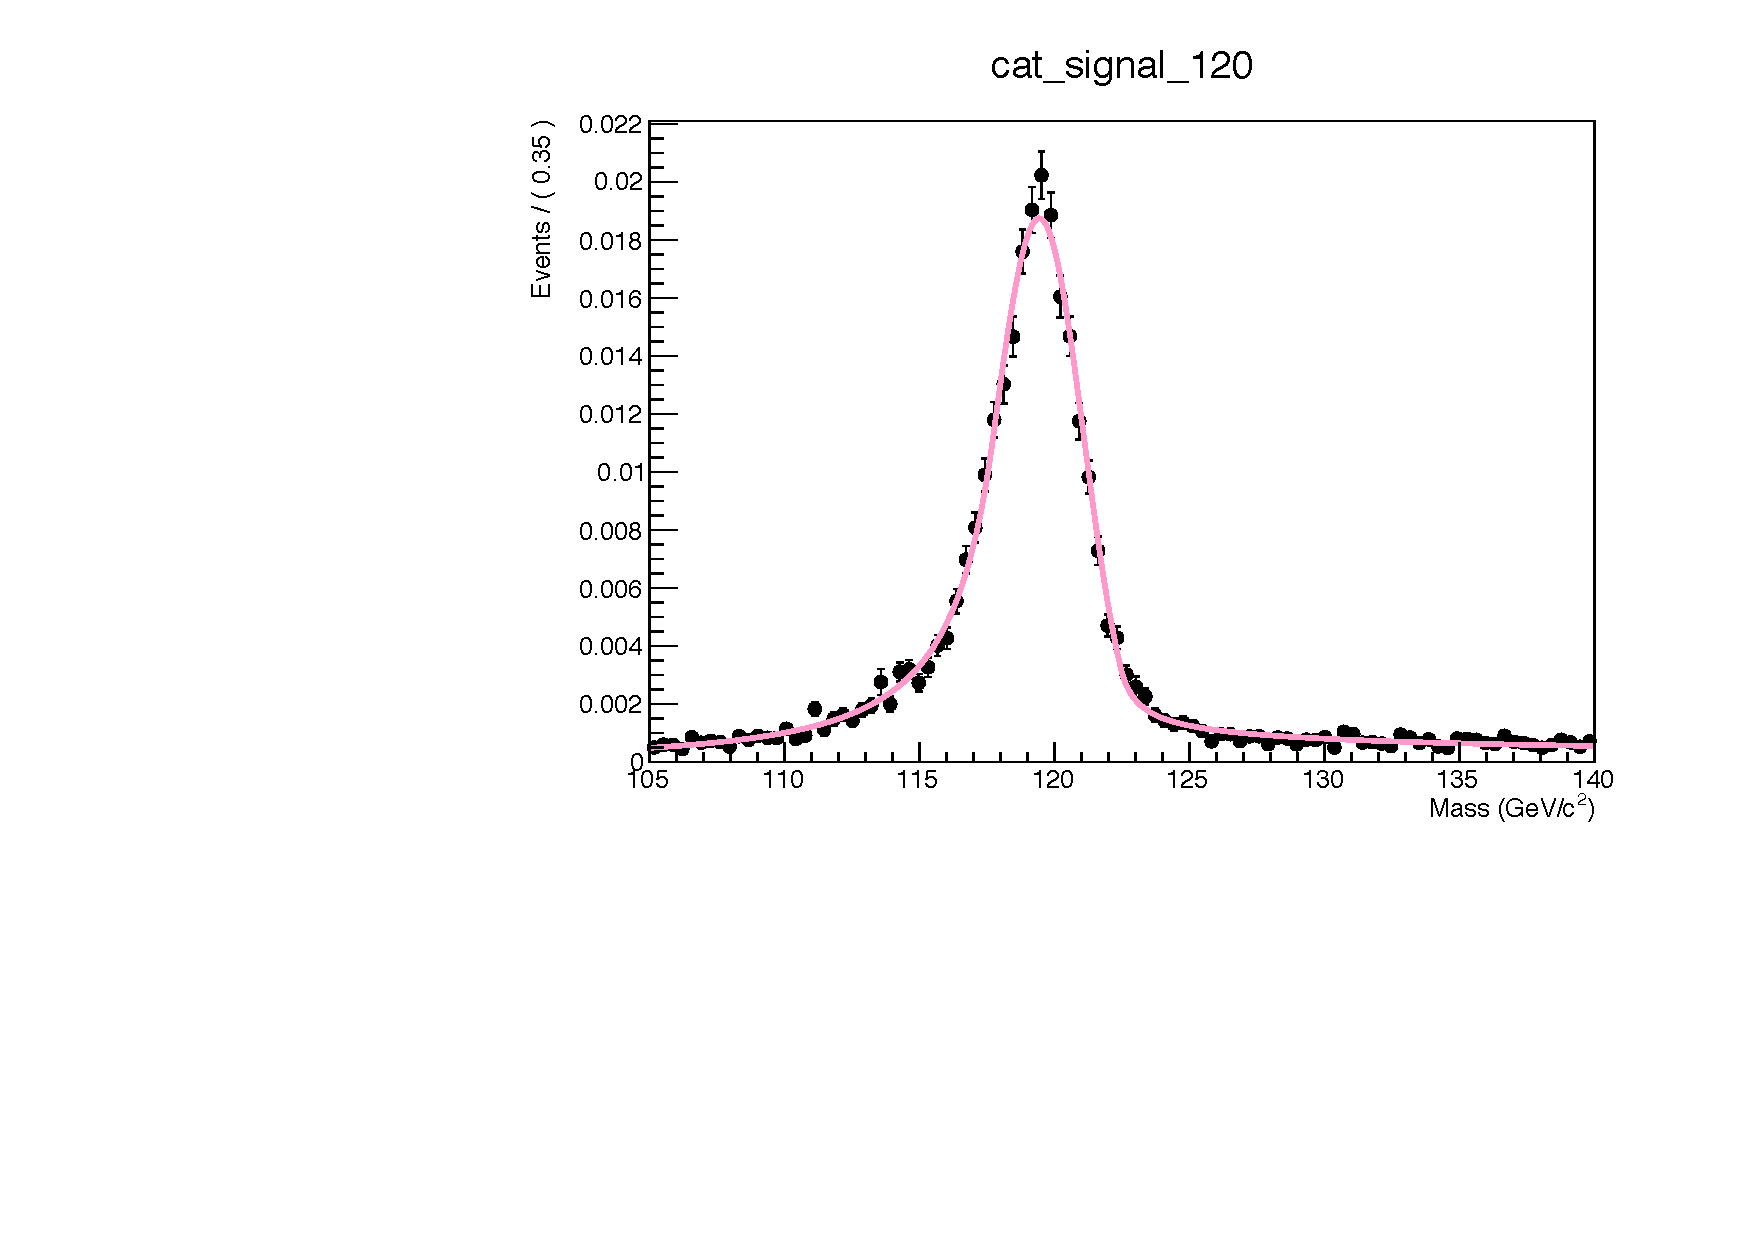
\includegraphics[width=0.3\textwidth]{Figures/SignalModelling/Signal_Parametrization/2018/ttH_2e2mu_2018_120_Sim.pdf} 
%		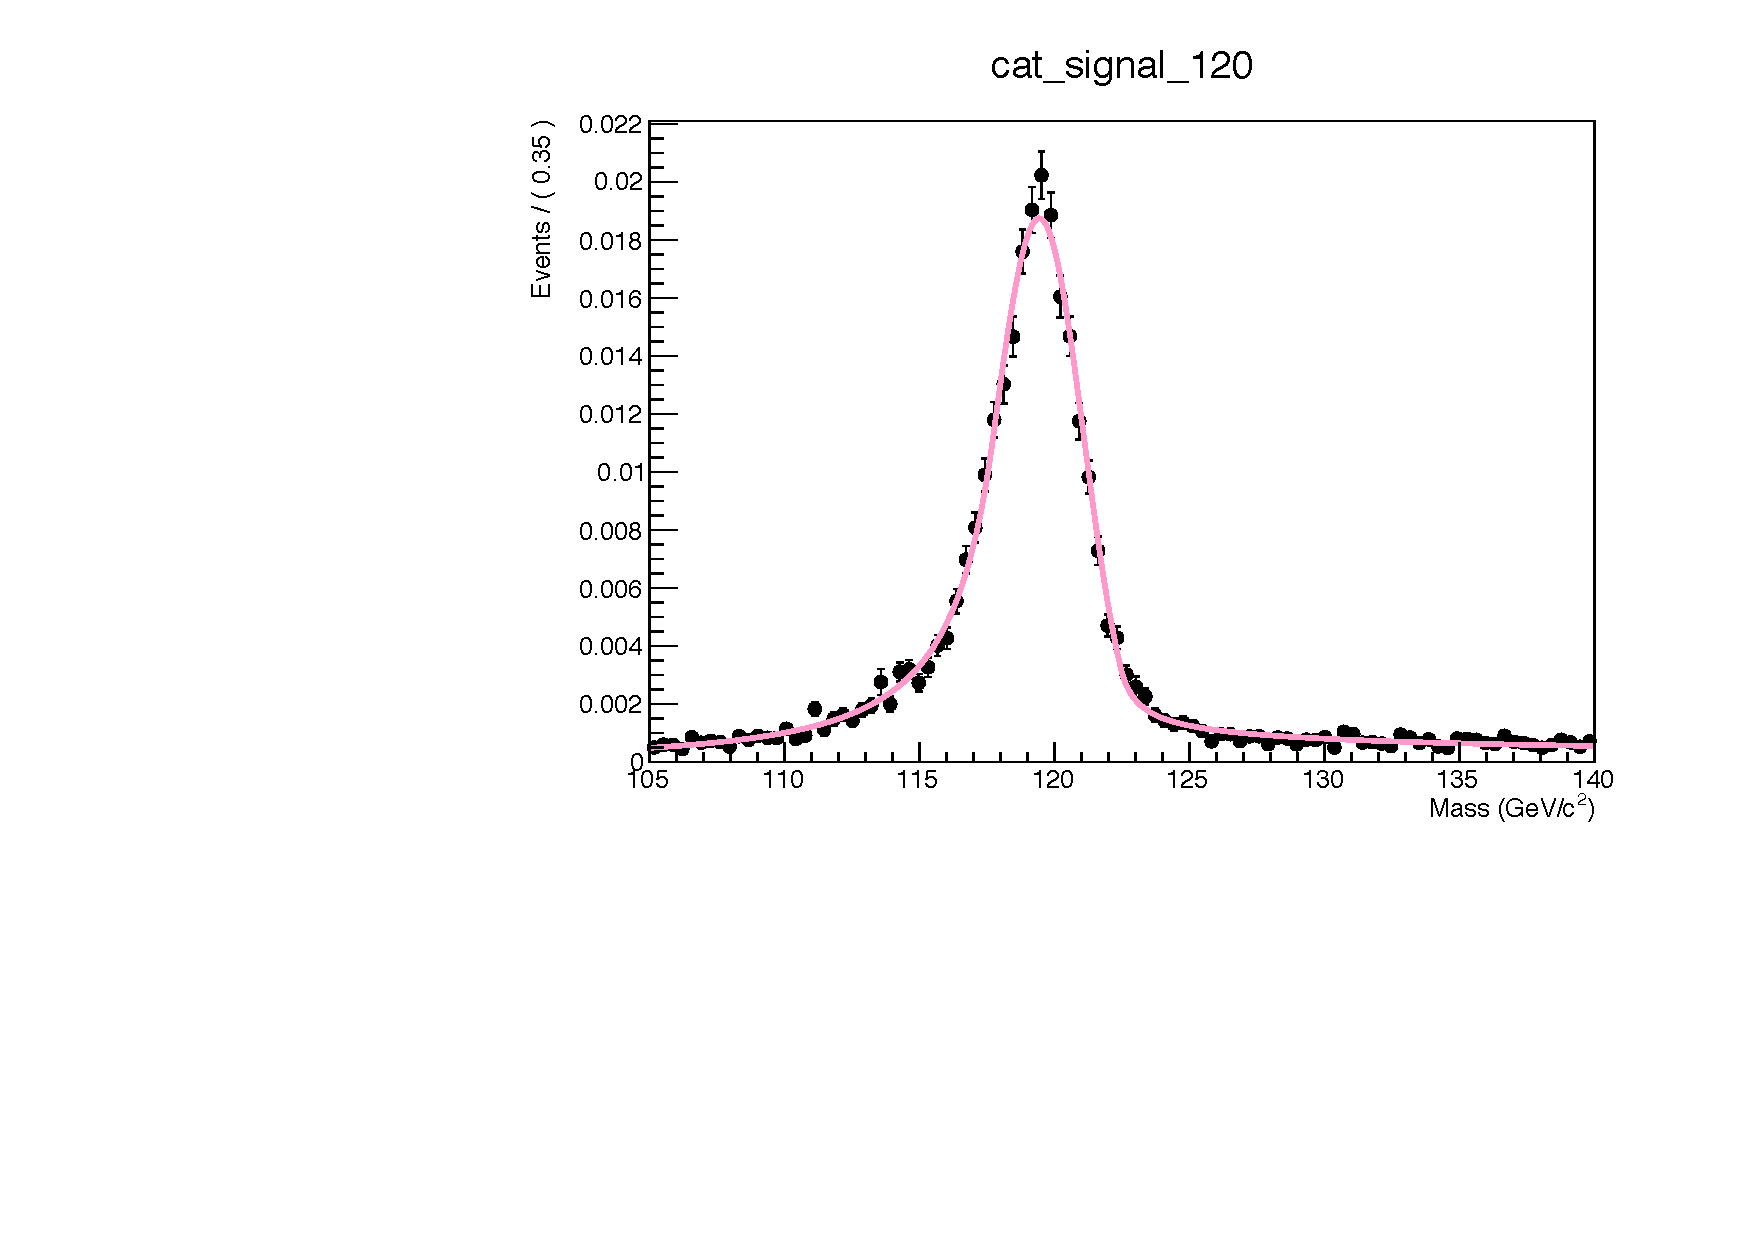
\includegraphics[width=0.3\textwidth]{Figures/SignalModelling/Signal_Parametrization/2018/ttH_2e2mu_2018_120_Sim.pdf}
%		\caption{Simultaneous fit for ggH production mode, in 2018, for different mass points, 
%		in 2e2$\mu$ final state.}
%	\label{signal_lineshape_2018_full_2}
%	\end{center}
%\end{figure}
\subsection{Building the 1D pdf}
The measurement of \mH is extracted by maximizing the one-dimensional likelihood function $\lhood \left( \mH \middlepipe \mfourl \right)$ using the \mfourl spectrum.  % TODO: Filippo has: "where $m_{H}$ is fixed to the value of 125 GeV." but this doesn't make sense. 
The model and the normalization used for the signal are described in Sec.~\ref{sec:SignalNormalization}.
The DSCB fits of the four-lepton invariant mass distributions are shown in Figure.~\ref{fig:1D_mass_2018_ggH} for the signal region 105--140\GeV using simulated ggH events, split into the four different final states.
% TODO: 2017 or 2016 plots?
\begin{multiFigure}
    \centering
    \addFigure{0.48}{../../higgsmassmeasurement/AN-19-248/Figures/ggH_MassDistribution/1D_mass_2018_ggH_4mu_workinprogress.pdf}
    \addFigure{0.48}{../../higgsmassmeasurement/AN-19-248/Figures/ggH_MassDistribution/1D_mass_2018_ggH_4e_workinprogress.pdf}
    \addFigure{0.48}{../../higgsmassmeasurement/AN-19-248/Figures/ggH_MassDistribution/1D_mass_2018_ggH_2e2mu_workinprogress.pdf}
    \addFigure{0.48}{../../higgsmassmeasurement/AN-19-248/Figures/ggH_MassDistribution/1D_mass_2018_ggH_2mu2e_workinprogress.pdf}
    \captionof{figure}
        [Distributions of \mfourl in the signal region (105--140\GeV) using simulated ggH events]
        {Distributions of \mfourl in the signal region (105--140\GeV) using simulated ggH events, fitted with a DSCB function using 2018 samples.
        \;A) \fourmu.
        \;B) \foure.
        \;C) \twoetwomu.
        \;D) \twomutwoe.
    }
    \label{fig:1D_mass_2018_ggH}
\end{multiFigure}

\subsubsection{Expected uncertainties on \mH before improvements}
Assuming perfect background rejection and neglecting any systematic uncertainties, the expected uncertainty on the measurement of \mH is shown in Tables~\ref{table:1D_model_result_fs} and~\ref{table:1D_model_result_year}, split by final state and by year, respectively.
% TODO: Consider using tabularx
%=== By final state.
\begin{table}[!ht]
    % \small
    \centering
    \topcaption
        [Expected Higgs boson mass uncertainty measured with the 1D model]
        {Expected Higgs boson mass uncertainty measured with the 1D model for different final states.
        All mass uncertainties are reported in $\MeVns$ and are statistical-only.
        }
	\begin{tabular}{cccccc}
            \hline      
        Expected uncertainty $(\MeVns)$	&	\fourmu	&	\foure	&	\twoetwomu	& \twomutwoe	& Inclusive	\\
            \hline
        1D	(No bkg) &	147	&	394	&	276	&	273	&	112	\\
            \hline
        \end{tabular}
    \label{table:1D_model_result_fs}
\end{table}
%=== By year.
\begin{table}[!ht]
    % \small
    \centering
    \topcaption
        [Expected Higgs boson mass uncertainty measured with the 1D model]
        {Expected Higgs boson mass uncertainty measured with the 1D model for different years during Run 2.
        All mass uncertainties are reported in $\MeVns$ and are statistical-only.
        }
	\begin{tabular}{|ccccc|}
            \hline      
        Expected uncertainty $(\MeVns)$	&	2016 pre-VFP	&	2016 post-VFP	&	2017	&	2018	\\
            \hline
        1D (No bkg)	&	304	&	314	&	207	&	170	\\
            \hline
        \end{tabular}
    \label{table:1D_model_result_year}
\end{table}
%The 1D likelihood scans vs \mH, while profiling signal strength $\mu$ as all other nuisance parameters, are 
%shown in \figurename~\ref{1D_model}. 
%%All systematic errors are included. In order to estimate the 
%%contribution of the statistical and systematic error to the mass measurement, a likelihood scan removing 
%%both the normalization and shape systematics is performed. As in the case of the scan including the full 
%%uncertainties, $\mu$ is profiled, and then its uncertainty is included in the statistical error, because 
%%its magnitude represents the amount of signal events fitted, and then it has statistical nature. 
%%The systematic uncertainty is estimated as the difference in quadrature between the full uncertainty 
%%and the statistical uncertainty. 
%Results are summarised in ~\tablename~\ref{table:1D_model_result}.
%\begin{figure}[!htbp]
%	\begin{center}
%		\includegraphics[width=0.35\textwidth]{Figures/Placeholder.png}
%		\includegraphics[width=0.35\textwidth]{Figures/Placeholder.png}
%		\caption{1D likelihood scan as a function of mass for 1D fit scenario for the combination of 
%		all final states (left). Solid lines represents the scan with full uncertainties included, 
%		dashed lines statistical error only.  Results for each final state is shown on the right.}
%		\label{1D_model}
%	\end{center}
%\end{figure}
%



%%%%%%% 
%%%%%%% 
% plots about normalisation will be shown only for 1D_VXBS_Z1 configuration
%%%%%%% 
%%%%%%% 
%Examples of the fit procedures are shown in \figurename~\ref{signal_lineshape_2016_width}, 
%\ref{signal_lineshape_2017_width},  \ref{signal_lineshape_2018_width}.
%\begin{figure}[!htbp]
%	\begin{center}
%   		\includegraphics[width=0.3\textwidth]{Figures/HiggsWidth/2016_4Mu.png}
%		\includegraphics[width=0.3\textwidth]{Figures/HiggsWidth/2016_4Ele.png}
%		\includegraphics[width=0.3\textwidth]{Figures/HiggsWidth/2016_2Ele2Mu.png}
%		\caption{Signal lineshape for 2016: 4$\mu$ on left, 4e in the middle, 2e2$\mu$ on right.}
%	\label{signal_lineshape_2016_width}
%	\end{center}
%\end{figure}
%\begin{figure}[!htbp]
%	\begin{center}
%   		\includegraphics[width=0.3\textwidth]{Figures/HiggsWidth/2017_4Mu.png}
%		\includegraphics[width=0.3\textwidth]{Figures/HiggsWidth/2017_4Ele.png}
%		\includegraphics[width=0.3\textwidth]{Figures/HiggsWidth/2017_2Ele2Mu.png}
%		\caption{Signal lineshape for 2017: 4$\mu$ on left, 4e in the middle, 2e2$\mu$ on right.}
%	\label{signal_lineshape_2017_width}
%	\end{center}
%\end{figure}
%\begin{figure}[!htbp]
%	\begin{center}
%   		\includegraphics[width=0.3\textwidth]{Figures/HiggsWidth/2018_4Mu.png}
%		\includegraphics[width=0.3\textwidth]{Figures/HiggsWidth/2018_4Ele.png}
%		\includegraphics[width=0.3\textwidth]{Figures/HiggsWidth/2018_2Ele2Mu.png}
%		\caption{Signal lineshape for 2018: 4$\mu$ on left, 4e in the middle, 2e2$\mu$ on right.}
%	\label{signal_lineshape_2018_width}
%	\end{center}
%\end{figure}
    